
\documentclass[master]{thesis-uestc}
\usepackage{listings}  % 引入 listings 宏包,用于显示代码
\title{面向长尾分布数据的自监督学习故障诊断方法研究}{}

\author{王本浩}{Wang Benhao}
\advisor{周雪\chinesespace 教授}{Dr. Xue Zhou}
\school{电子科技大学(深圳)高等研究院}{Shenzhen Institute for Advanced Study, UESTC}
\major{电子信息}{Electronic Information}
\studentnumber{202222280517}

\begin{document}

\makecover

\begin{chineseabstract}
    随着现代工业系统日益复杂化,单一系统中的故障类型也呈现出不断增长的趋势,导致数据集常常呈现长尾分布。在此背景下,传统的智能故障诊断模型往往存在偏向将尾部类样本错误分类为头部类样本的问题。然而,尾部类中的罕见故障类型通常对系统的危害更大,因此,它们在故障诊断中的价值更为突出。自监督学习已成为解决长尾分布问题的主流方法,其训练过程分为自监督预训练和微调两个阶段。自监督预训练阶段利用无标签数据集和代理任务对模型特征层进行训练,微调阶段则在有标签数据的基础上,通过在特征层上附加线性分类层来训练最终的分类模型。
    本文旨在研究面向长尾分布数据的自监督学习故障诊断方法,主要内容包括:(1)基于孪生网络对比学习的自监督预训练方法;(2)结合半监督学习与MARC决策面校准算法的微调方法。我们的方法在构建的长尾分布CWRU轴承故障诊断数据集上,成功超越了现有SOTA方法SimCLR和BYOL,取得了更优的性能。希望该方法能够为致力于解决长尾分布问题的研究人员提供新的思路和启示。

\chinesekeyword{故障诊断,长尾学习,自监督学习,孪生网络,半监督学习,决策面调整}
\end{chineseabstract}

\begin{englishabstract}
    With the increasing complexity of modern industrial systems, the types of faults within a single system have also grown, and datasets often exhibit a long-tail distribution. This results in traditional intelligent fault diagnosis models having a bias towards classifying tail-class samples as head-class samples. However, it is often the rare faults in the tail classes that pose a greater threat to the system, making these rare faults more valuable for diagnosis. The self-supervised learning paradigm is a mainstream solution to the long-tail distribution problem. It divides model training into two stages: self-supervised pretraining and fine-tuning. In the pretraining stage, the model's feature layer is trained using an unlabeled dataset and a proxy task. In the fine-tuning stage, the final classification model is trained using labeled data and a linear classification layer added to the feature layer. This paper focuses on self-supervised learning methods for fault diagnosis on long-tail distribution data, and its main contributions are: (1) a self-supervised pretraining method based on Siamese network contrastive learning, and (2) a fine-tuning method combining semi-supervised learning with MARC margin calibration. Our method achieves superior performance on the constructed long-tail distribution CWRU bearing fault diagnosis dataset, surpassing existing SOTA methods such as SimCLR and BYOL. We hope this method can provide ideas and insights for researchers addressing long-tail distribution problems.

\englishkeyword{Fault Diagnosis, Long-Tail Learning, Self-Supervised Learning, Siamese Network, Semi-Supervised Learning, Margin Calibration}
\end{englishabstract}

\thesistableofcontents

\chapter{绪\hspace{6pt}论}

\section{研究工作的背景与意义}
旋转机械作为现代工业中的关键设备,长期在高温、疲劳、重载等复杂环境中运行。故障的发生可能导致严重事故,带来巨大的经济损失和人员伤亡。智能诊断是预测健康管理(PHM)系统的关键组成部分,PHM在直升机、航空发动机、风力涡轮机、高速列车等旋转机械中发挥着至关重要的作用,其核心目标是有效地检测故障。传统的智能诊断方法主要包括信号处理技术用于特征提取,以及机器学习方法用于故障分类,这些方法已经取得了显著进展。然而,面对异构且海量的数据,依赖专家设计和选择的特征提取方法,及从信号到条件的映射能力,在很大程度上依赖先验知识,这不仅耗时而且需要丰富的经验。因此,如何更精确、更高效地进行故障诊断仍然是一个具有挑战性的课题。

现实中的故障检测数据通常呈现长尾分布\citing{nanjing2023faultdetection},这是一种偏态分布,其中头部类包含大量正常数据,而尾部类则包含较少的故障数据。在使用长尾数据训练神经网络时,模型的性能容易受到头部类的影响,从而在尾部类上表现较差。尾部类的错分往往带来更大的损失,因此,尾部类样本的研究具有重要的价值意义。如何基于长尾分布的故障检测数据训练有效的故障检测模型,是一个具有现实意义的难点问题\citing{cumm2023faultdiagnosis}。

目前,在视觉识别领域,长尾学习已提出多种前沿方法,如变分自编码器\citing{kingma2013auto}、生成对抗网络\citing{goodfellow2020generative}、CB(Class-Balanced)Loss\citing{cui2019class}、自监督学习\citing{yang2020rethinking}、以及MARC决策面调整算法\citing{wang2023margin}等。然而,在故障诊断的长尾学习领域,常见的方案包括半监督学习\citing{nanjing2023faultdetection}、集成学习\citing{吴亮2023基于多级学习的长尾分布下交通多目标检测}、样本加权\citing{cumm2023faultdiagnosis}等,相较而言,前沿的长尾学习方法在故障诊断中的应用较少。因此,提出一个结合前沿长尾学习方法的故障诊断模型具有重要的现实意义。

当前,大多数神经网络训练仍依赖有监督学习范式,需要大量的标注数据,而数据标注既费时又费力。自监督学习的提出旨在突破对人工标注的依赖,使得即使在没有标注数据的情况下,也能高效地训练网络。与传统的无监督学习不同,自监督学习通过人工构造输入数据的代理标签,并依托代理标签设计神经网络的监督训练任务,从而使网络学习到有效的特征表示。文献\cite{zhang2021federated}指出,额外的自监督预训练能够显著提升常规长尾学习算法的性能,并已在CIFAR-LT、ImageNet-LT等视觉识别长尾数据集上得到验证。尽管在故障诊断的长尾学习领域,半监督学习、集成学习、样本加权等方法已经取得一定进展,但应用自监督预训练方法的研究仍相对较少。因此,基于自监督预训练的长尾数据故障诊断仍是一个具有重要挑战的研究方向。

\section{长尾学习方法的国内外研究历史与现状}
\subsection{长尾学习的发展历程和研究现状}
国内外在处理长尾问题时通常从三个方面着手:一是样本层面,采取欠采样(如随机欠采样、NearMiss\citing{shen2016near}、ENN\citing{wilson1972asymptotic})或过采样(如随机过采样、SMOTE\citing{chawla2002smote}、变分自编码器\citing{kingma2013auto}、生成对抗网络\citing{goodfellow2020generative})的方法。然而,由于新生成的样本中可能包含噪声,模型仍然容易出错。;二是损失函数层面,使用类平衡的损失函数,如基于数据频率逆加权\citing{huang2016learning},OHEM(Online Hard Example Mining)、Focal Loss\citing{lin2017focal},以及最新提出的CB(Class-Balanced)Loss\citing{cui2019class};三是模型层面,如通过集成学习、半监督和自监督学习\citing{yang2020rethinking}、MARC决策面调整算法\citing{wang2023margin},采用少数类样本与等量多数类样本的组合进行模型训练,还有迁移学习\citing{liu2019large,yin2019feature}、度量学习\citing{you2018scalable,zhang2017range} 和元学习\citing{jamal2020rethinking,shu2019meta},也得到了探索。最近的研究还发现,解耦特征层与分类器的结构可以带来更好的长尾学习结果\citing{zhou2020bbn, kang2019decoupling}。

在长尾分布问题的研究上,国内外已有大量的探索。例如,Liu J等人\citing{liu2020deep}提出了一种基于特征云的数据增强方法,通过从方差较大的头部类中学习类内多样性,并将其转移到尾部类,从而改善尾部类的分类效果,该方法已成功应用于人脸识别领域。Yang Y等人\citing{yang2020rethinking}探讨了不平衡样本标签在模型训练中的价值,提出通过半监督学习方法利用原模型识别无标签数据,并通过伪标签扩充原数据集,同时验证了自监督预训练在长尾学习中的有效性,且证明样本维度越高,性能提升越显著。吴磊等人\citing{wu2023personalized}提出了一种面向长尾图像的个性化专家识别算法,基于残差网络构建多专家学习网络,并加入个性化学习模块、信息融合模块及个性化信息增强模块,通过两阶段学习显著提升了长尾图像整体的识别精度,特别是中、尾部类别的识别效果。吴亮等人\citing{吴亮2023基于多级学习的长尾分布下交通多目标检测}提出了多级分组分类器,以提升尾部类性能,同时避免头部类性能损失,并设计了基于多头注意力机制的分组特征重融合模块,为多级分类器输入更精细的特征。此外,基于多级分类器,他们还提出了Logit联合调整方法,以缓解组间不平衡问题。Wang Y等人\citing{wang2023margin}介绍了适用于长尾视觉识别的MARC决策面调整算法,通过对模型输出的预测分数进行额外训练,仅需三行代码便能实现。Cui Y等人\citing{cui2019class}提出了CB(Class-Balanced)损失函数,通过乘以与“独特”样本数量相关的因子,缓解了类别不平衡问题。CB因子与超参数β有关,通过平滑1到最常见类别的不平衡因子1/n来实现。

综上所述,文献\cite{yang2020rethinking}为自监督预训练在故障诊断长尾学习中的应用提供了良好的启示,但半监督学习方法在现实长尾学习模型中的适用性尚待验证。文献\cite{wu2023personalized,吴亮2023基于多级学习的长尾分布下交通多目标检测}介绍的集成学习方法有助于减弱样本不平衡效应,虽然是常规方法,但如果在训练过程中融合自监督预训练,性能可能会得到进一步提升。文献\cite{wang2023margin}提出的决策面调整算法适用于一般长尾学习模型,但其在故障诊断中的可行性仍需进一步探讨,且该算法对模型性能提升的理论性解释也尚不完善。文献\cite{cui2019class}提出的损失函数方法具有创新性,但超参数β的人工选择在实际应用中可能面临一定的挑战。以上研究多集中于视觉长尾学习领域,并且在CIFAR-LT、ImageNet-LT等视觉识别数据集上取得了良好效果,而在故障诊断长尾学习领域,前沿的长尾学习算法应用较为匮乏。因此,将前沿的长尾学习算法应用于故障诊断领域,具有重要的研究价值。

\subsection{自监督预训练的发展历程和研究现状}

2019年,MoCo\citing{He_2020_CVPR}的提出掀起了视觉自监督学习的热潮,随后SimCLR\citing{chen2020simple}、BYOL\citing{grill2020bootstrap}、SwAV\citing{caron2020unsupervised}等主流自监督学习算法相继问世,使得该领域呈现出百花齐放、百家争鸣的繁荣局面。2021年末,MAE\citing{he2022masked}的提出进一步推动了自监督学习的发展,使其达到了前所未有的新高度。然而,这一成就的背后,自监督学习经历了长期的迭代与发展。

目前,国内外学者对自监督预训练方法展开了大量研究。例如,在计算机视觉领域,Yang等人\citing{yang2020rethinking}研究了不平衡样本标签信息在模型训练中的价值,提出了一种半监督学习方法,该方法通过利用原模型识别无标签数据并生成伪标签来扩充原数据集,并验证了自监督预训练的有效性。此外,该研究还发现,样本维度越高,性能提升越显著,这为自监督预训练在故障诊断长尾学习领域的应用提供了有力支持。Doersch等人\citing{doersch2015unsupervised}提出了基于局部图像块位置预测的自监督任务,随机抽取图像中的两个块,训练模型预测一个块相对于另一个块的位置。Zhang等人\citing{zhang2016colorful}构建了基于图像上色的自监督任务,将图像转换至CIE Lab颜色空间,利用L通道作为输入,让模型预测a和b通道的颜色信息。Gidaris等人\citing{gidaris2018unsupervised}通过人为旋转图像不同角度,并将旋转角度作为监督信号训练模型,从而实现图像语义特征的自监督学习。文献\cite{noroozi2017representation}提出了一种新的表示学习方式,通过基于计数视觉原语的人工监督信号来进行训练,而无需任何人工标注。核心思想是利用图像变换与表示变换之间的等变关系。文献\cite{caron2018deep}提出了利用KMeans算法生成样本的伪标签,将其作为数据的真实标签训练网络,用网络新提取的特征重新生成KMeans伪标签,以此重复。

近年来,自监督预训练方法也逐步应用于故障诊断领域,并受到广泛关注。例如,Zhang等人\citing{zhang2022prior}提出了基于先验知识的自监督任务,利用卷积自编码器进行训练,在小样本学习任务中取得了良好表现。Senanayaka等人\citing{senanayaka2020toward}采用One-Class SVM输出的标签作为代理标签,使用自监督预训练的卷积神经网络进行故障特征提取。W. Zhang等人\citing{zhang2021federated}提出了一种基于信号块交换的自监督任务,即通过打乱时域信号块顺序构造“伪数据”,并训练模型区分原始数据和伪数据。实验结果表明,该方法在特征提取任务中表现优异。

综上所述,尽管文献\cite{doersch2015unsupervised, zhang2016colorful, gidaris2018unsupervised}等研究在计算机视觉领域取得了重要进展,但其方法在故障诊断任务中的直接应用仍面临一定困难。然而,这些研究的思路为故障诊断领域的自监督预训练任务设计提供了有益的启示。例如,文献\cite{senanayaka2020toward}提出的One-Class SVM生成的标签可以结合聚类算法,使其适用于多分类任务;文献\cite{zhang2021federated}提出的信号块交换方法与文献\cite{doersch2015unsupervised}提出的图像块位置预测任务在思路上具有一定相似性,值得探索其结合的可能性。此外,文献\cite{zhang2022prior, senanayaka2020toward, zhang2021federated}提出的自监督预训练方法在任务设计上仍具有较大的创新空间,且在长尾学习任务中的应用尚未得到充分探索。因此,故障诊断领域的自监督预训练仍处于发展初期,借鉴计算机视觉领域的前沿自监督任务,提出更具创新性和更高性能的自监督预训练任务,仍具有重要的研究价值和挑战。

\subsection{对比自监督学习的发展与孪生网络的应用}

自监督学习的核心目标是在无人工标注的情况下自动提取有效特征\citing{min2021cross}。近年来,对比自监督学习(contrastive self-supervised learning)作为无监督学习的一个重要分支,逐渐成为研究热点,并在图像识别任务中取得了最先进的(SOTA)性能。许多相关算法相继被提出,例如动量对比学习(Momentum Contrast, MoCo)\citing{He_2020_CVPR}、对比预测编码(Contrastive Predictive Coding, CPC)\citing{oord2018representation}以及用于视觉表征学习的简单对比学习框架(SimCLR)\citing{chen2020simple}。

这些方法的核心思想是通过拉近相同样本的不同视图(正样本对)并推远不同样本(负样本对)来学习有意义的特征表示。对比学习方法通常依赖存储在记忆库(memory bank)中的大量负样本,以提高对比学习效果\citing{wu2018unsupervised}。此外,一些其他对比学习方法不依赖负样本,而是计算两个正样本对之间的相似性,例如SwAV(Swapping Assignments between multiple Views)\citing{caron2020unsupervised}、BYOL(Bootstrap Your Own Latent)\citing{grill2020bootstrap}以及SDCT(Self-supervised Deep Correlation Tracking)\citing{yuan2020self}。

在对比自监督学习中,孪生网络(Siamese Network)因其适用于比较不同样本的网络结构,具有独特优势。Laine和Aila\citing{laine2016temporal}提出了基于孪生网络的$\pi$-model,用于训练深度神经网络,该方法在半监督学习场景下依赖不同的正则化规则与数据增强策略。Zheng和Yang\citing{zheng2019unsupervised}提出了一种“记忆正则化”机制,其核心思想是让主模型自身(而非外部模块)学习域内知识,以实现无监督场景自适应。Zhao等人\citing{zhao2021deep}提出了基于相互学习(mutual learning)和知识蒸馏(knowledge distillation)的训练方法,以提高视觉目标跟踪任务的性能。

上述研究均在各自领域中引入孪生网络的思想,以解决特定问题。本文受到SimSiam\citing{chen2021exploring}的启发,SimSiam采用简化的孪生网络结构,并在计算机视觉(CV)任务中展现出卓越性能。基于此,我们提出了一种新颖的轴承故障诊断框架,该框架可适用于由不同神经网络层构建的多种模型。与其他主流方法相比,SimSiam 具有以下三大优势:
\begin{enumerate}
    \item 无需构造负样本对;
    \item 无需采用大批量训练;
    \item 无需使用动量编码器(momentum encoder)。
\end{enumerate}


\section{本文的主要贡献与创新}

本论文聚焦于面向长尾分布数据的自监督学习故障诊断,主要的创新点和贡献如下:

\begin{enumerate}
    \item 提出了基于SimSiam简单孪生网络的自监督预训练故障诊断框架。
    \item 提出了基于CMA-ES算法搜索最优数据增强策略的方案。
    \item 提出了结合半监督学习与MARC决策面调整的微调算法。
\end{enumerate}

\section{本论文的结构安排}

本文的章节结构安排如下:

第一章介绍了研究的背景与意义,分析了传统故障诊断方法在处理长尾分布数据时面临的挑战,并重点回顾了国内外在长尾学习算法领域的研究进展与现有局限性。

第二章阐述了长尾学习与自监督学习范式的基本概念,介绍了为提出SimSiam简单孪生网络故障诊断框架的理论基础,并介绍了实验使用的数据集和研究对象。

第三章提出了基于SimSiam简单孪生网络为骨干网络的自监督预训练故障诊断框架,详细描述了框架各模块的设计与实现,并从实验与理论两个层面验证了框架的有效性。通过准确率、t-SNE分布图以及对Batch Size等参数的敏感性分析,证明了该方法在性能和稳定性上优于现有SOTA的自监督学习方法。

第四章提出了基于半监督学习与MARC决策面调整相结合的微调框架,旨在减轻SimSiam网络在微调阶段受长尾效应影响的问题。实验结果表明,该微调框架不仅提升了SimSiam网络的整体性能,而且在其他模型中同样具有较好的效果,展示了其良好的普适性。

第五章对全文工作进行了总结,并对未来的研究方向进行了展望。


\chapter{长尾学习及相关方法的理论基础与轴承故障数据集}
\section{长尾学习相关理论}
不平衡数据在现实世界中广泛存在,大规模数据集通常呈现出长尾分布的特性。长尾分布的学习是故障诊断领域中的一项常见挑战。例如,正常工作状态的数据通常远多于故障工作状态,或者常见故障状态的数据量远多于罕见故障状态。现实中的故障检测数据往往服从长尾分布,这种分布是一种典型的偏态分布,如图\ref{fig_long_tail}所示:大规模训练数据中,头部类别的样本数量占据主导地位,而尾部类别的样本数量相对稀少,并呈现逐渐递减的趋势。在使用长尾数据训练神经网络时,模型性能容易受到头部类别的影响,导致尾部类别的表现较差。然而,对尾部类别样本的错分往往带来更大的实际损失,因此研究尾部类别样本具有重要的现实意义。如何基于长尾分布的故障检测数据有效训练故障检测模型,已成为一个具有重要价值的研究难题。
\begin{figure}[h]
    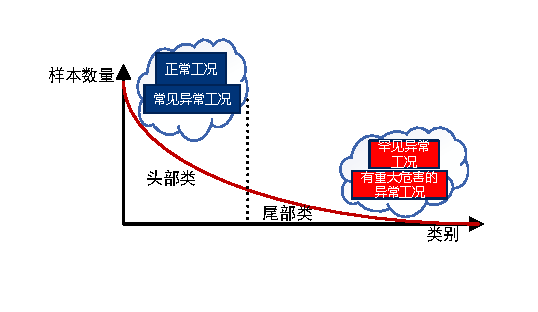
\includegraphics[width=10cm]{long_tail.pdf}
    \caption{长尾分布示意图}
    \label{fig_long_tail}
\end{figure}

长尾分布的数据存在显著的样本不均衡问题,导致训练的模型易偏向头部类别,从而削弱了对尾部类别的识别能力。如图\ref{tsne_mean_distribution}所示,当样本分布均衡时,各类别在特征空间中具有清晰的区分边界,并占据较宽广的特征空间。然而,当数据分布失衡呈现长尾分布时(如图\ref{tsne_lt_distribution}所示),尾部类别的特征分布变得狭窄,并依附于头部类别附近,从而扭曲了特征空间结构,降低了类别间的多样性与区分性。

这种不均衡数据对现代深度学习框架提出了巨大的挑战。即使使用数据重采样、类平衡损失等专门技术,在极端类不平衡的情况下,模型性能仍然显著下降。因此,为了更有效地应对这一挑战,深入理解类不平衡学习对特征分布的影响至关重要。

然而,与平衡数据的学习情景不同,不平衡学习中的标签扮演着一个复杂而矛盾的角色,形成了标签价值的困境。一方面,有标签的监督学习通常比无监督学习能够训练出更准确的分类器,这突显了标签的积极作用;另一方面,不平衡的标签分布会自然引入“标签偏差”,其中头部类别在很大程度上驱动决策边界的学习,导致对尾部类别的压制。这表明,不平衡标签既是推动学习的动力,也可能成为性能下降的原因,具有双刃剑的特性。
\begin{figure}[h]
    \subfloat[]{
        \label{tsne_mean_distribution}
        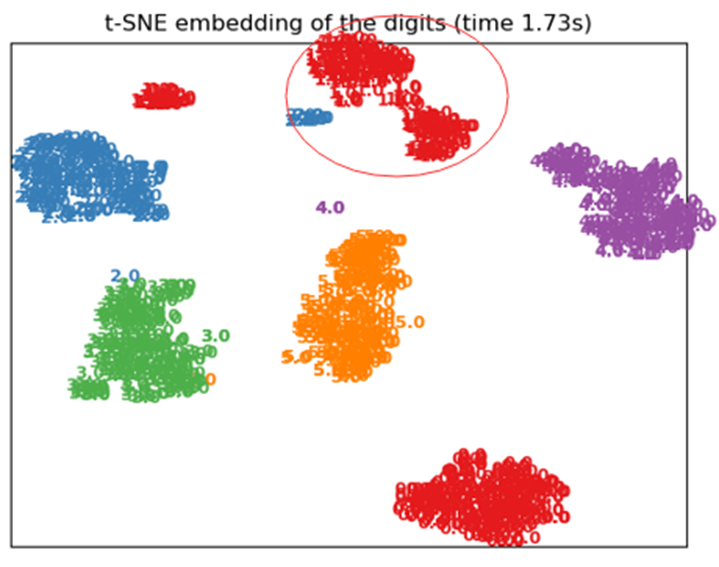
\includegraphics[width=6.77cm]{tsne_mean_distribution.png}
    }
    \subfloat[]{
        \label{tsne_lt_distribution}
        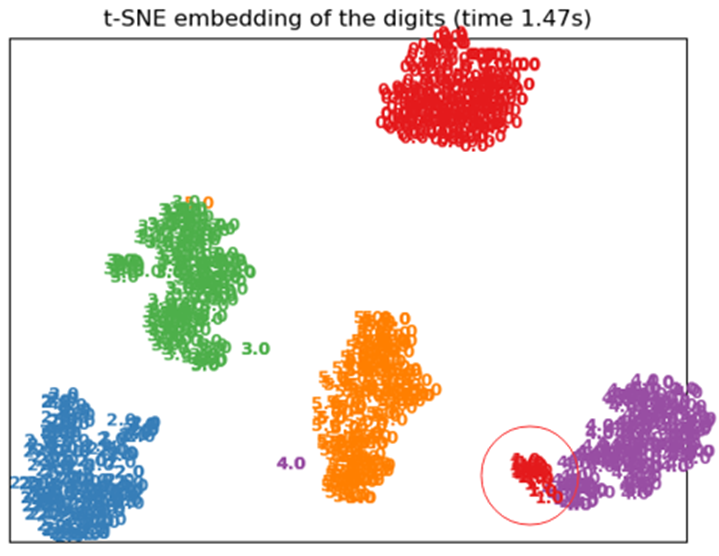
\includegraphics[width=6.77cm]{tsne_lt_distribution.png}
    }
    \caption{均匀/长尾分布数据的tsne图(a)样本均匀分布时的T-SNE分布图;(b)尾部类“1”类样本个为30,头部类样本个数为180个时的T-SNE分布图}
    \label{long-tail result}
\end{figure}

\section{自监督学习相关理论}
自监督学习是一种范式,利用“代理任务”(pretext)从大规模的无标签数据本身的内在结构挖掘通用的表征信息,通过这种构造的监督信息对网络进行训练,从而可以学习到对下游任务有价值的表征。如图\ref{self_supervise_procedure}所示,自监督学习分为两个阶段:(1)自监督预训练阶段。完全放弃标签信息,专注于数据本身,通过自监督学习进行预训练。从不平衡数据中学习标签不可知的特征表示,减少类别偏差对初始化的影响。(2)微调阶段。使用第一阶段中通过自监督预训练的网络权重作为初始化。在此基础上,可以使用任何标准的不平衡学习技术进行进一步训练,学习最终的分类模型。由于预训练阶段和正常训练阶段是独立的,自监督学习可以与现有的不平衡学习方法无缝结合,增强模型性能,且自监督预训练阶段不依赖标签,使得网络能学习到更通用、更鲁棒的特征表示,从而避免了类别不平衡对特征学习的负面影响。
\begin{figure}[h]
    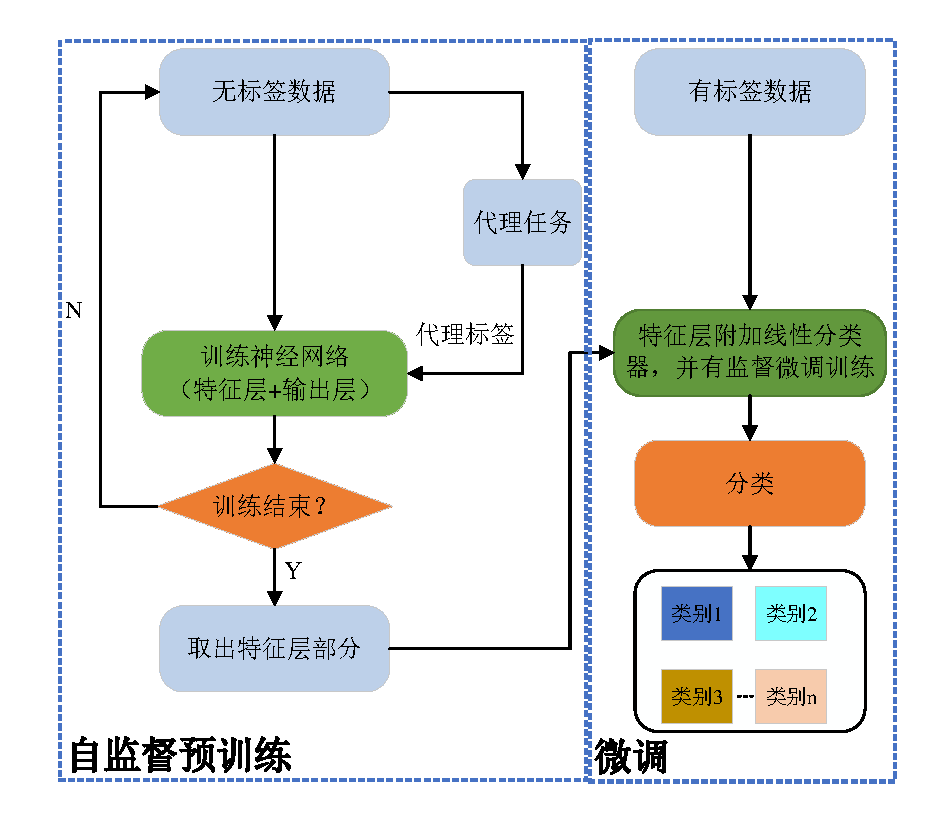
\includegraphics[width=10cm]{self_supervise_procedure.pdf}
    \caption{自监督训练范式流程}
    \label{self_supervise_procedure}
\end{figure}

\section{孪生网络与对比学习相关理论}
对比学习是一种通过比较正负样本对来提取有意义特征的学习方法。其基本假设是在学习到的嵌入空间中,相似样本应聚集在一起,而不相似样本应远离彼此。通过将学习任务视为辨别任务,对比学习能够帮助模型识别数据中的潜在特征和相似性。对比学习可分为监督对比学习和自监督对比学习两类。

监督对比学习是对比学习的一个子领域,依赖于标注数据来明确区分相似与不相似的样本。在监督对比学习中,模型通过训练数据对及其对应标签来学习哪些数据点是相似的,哪些是不相似的。其目标是学习一个表示空间,其中相似的实例聚集在一起,而不相似的实例则被推开。常见的优化目标是信息噪声对比估计(InfoNCE)损失函数,该函数最大化正样本对之间的相似性,同时最小化负样本对之间的相似性。通过优化该目标,模型能够有效区分正负样本,进而提升下游任务的性能。

自监督对比学习则不同于监督学习,它从未标注的数据中学习有效的特征表示。自监督对比学习通过设计代理任务,从未标注数据中生成正负样本对。这些代理任务旨在促使模型捕获数据中有意义的特征和相似性。自监督对比学习中的一种常见方法是通过数据增强生成同一实例的多个视图,并将这些视图作为正样本对,而来自不同样本的实例则作为负样本对。通过训练模型区分这些正负样本对,模型能够学习到更丰富的语义信息,并在下游任务中取得较好的推广效果。

\section{CWRU数据集介绍}
\begin{figure}
    \centering
    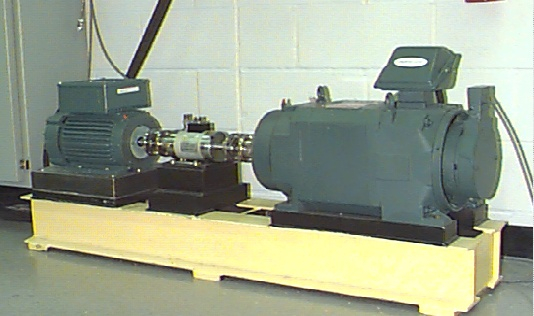
\includegraphics[width=6cm]{cwru_device.jpeg}
    \caption{CWRU轴承测试设备}
    \label{cwru_device}
\end{figure}
数据集由 CWRU(Case Western Reserve University)提供。图 \ref{cwru_device} 显示了测试设备,该设备包含一台 2 马力电机、一个扭矩编码器、一个测功机以及一些控制电路。测试使用的轴承为 6205-2RS JEM 深沟球轴承,分别安装在电机的驱动端和风扇端。  

轴承故障是通过单点电火花放电加工(Electro-discharge Machining)制造的。根据故障位置,故障类型可分为以下四种:  
1) 外圈故障(Outer Raceway Fault, OF);  
2) 内圈故障(Inner Raceway Fault, IF);  
3) 滚动体故障(Roller Faults, RFs);  
4) 正常状态(Normal Condition, NC)。  
轴承故障的严重程度可由故障直径(Fault Diameter)描述,故障直径指轴承或其他机械部件上出现的故障或损伤的直径尺寸。 故障直径通常用来描述故障的大小和程度,对于故障诊断和预测维护非常重要。

本研究采集了安装在驱动端的轴承数据,采样频率为 12 kHz,故障直径分别为 0.007 英寸,0.014英寸和0.021英寸的内圈故障、外圈故障、滚动体故障。不同故障类型的波形如图 \ref{cwru_samples} 所示。有关该数据集的更多详细信息,可访问 CWRU 轴承数据中心网站\citing{loparo2012case}。  

\begin{figure}
    \centering
    \subfloat[]{
        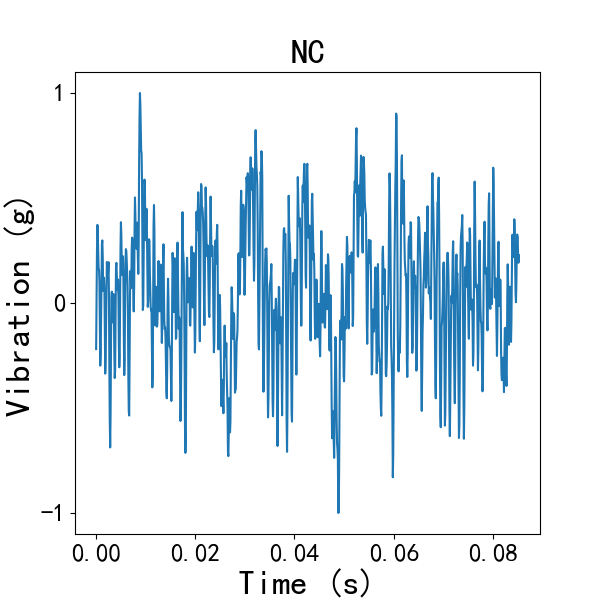
\includegraphics[width=0.28\linewidth]{class_0.png}
        \label{class_0}
    }
    \subfloat[]{
        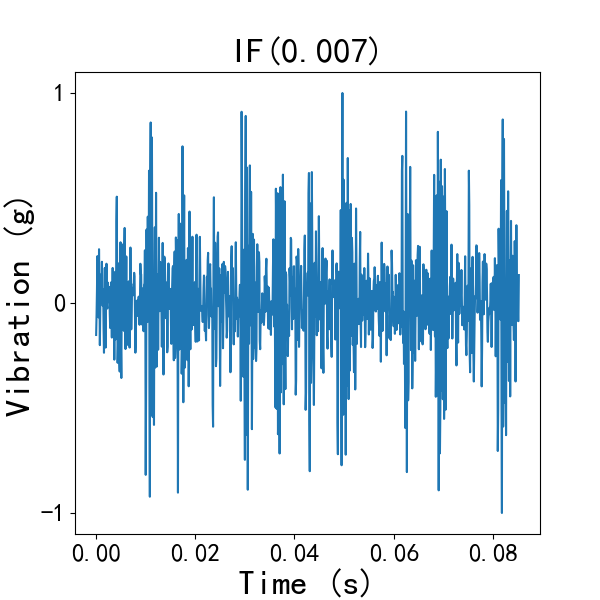
\includegraphics[width=0.28\linewidth]{class_1.png}
        \label{class_1}
    }
    \subfloat[]{
        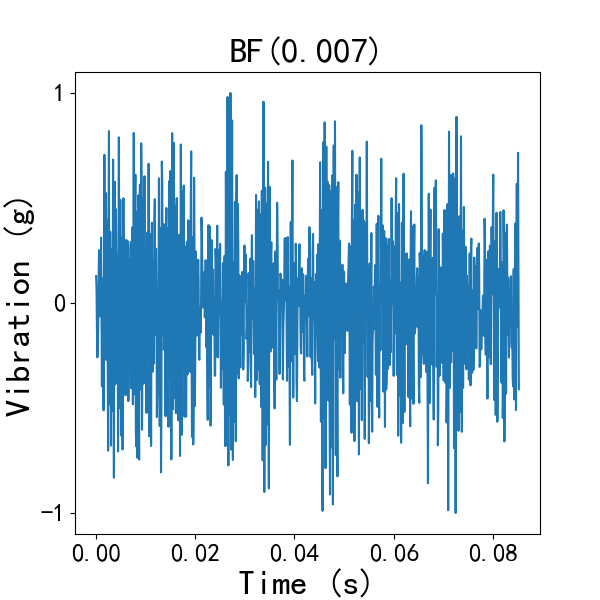
\includegraphics[width=0.28\linewidth]{class_2.png}
        \label{class_2}
    }
    \\ % 换行
    \subfloat[]{
        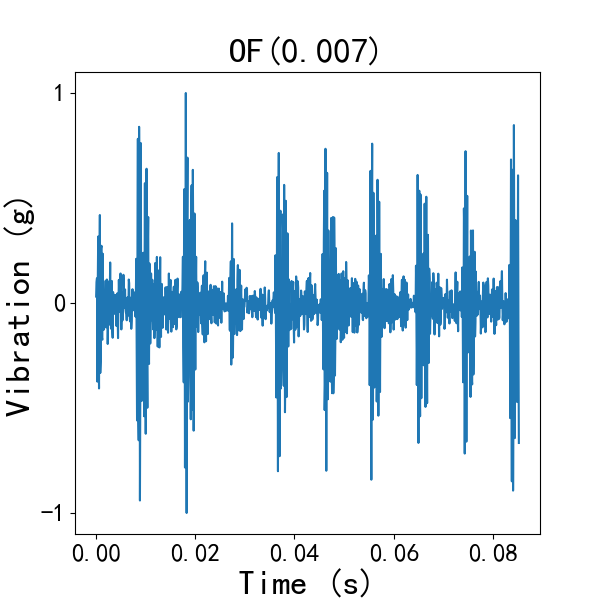
\includegraphics[width=0.28\linewidth]{class_3.png}
        \label{class_3}
    }
    \subfloat[]{
        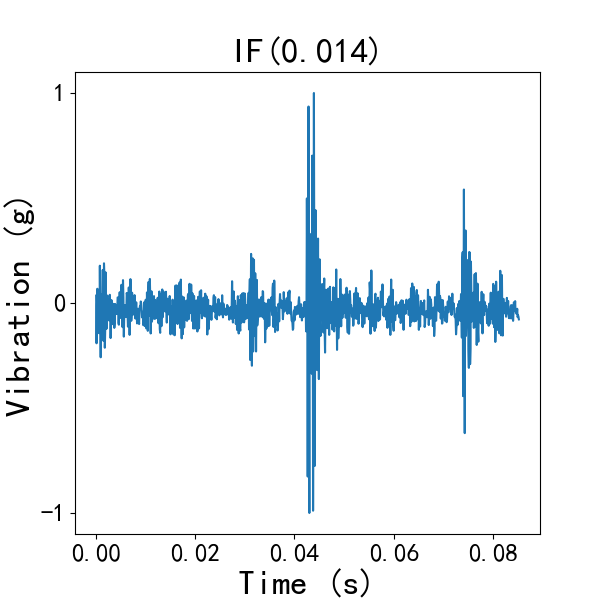
\includegraphics[width=0.28\linewidth]{class_4.png}
        \label{class_4}
    }
    \subfloat[]{
        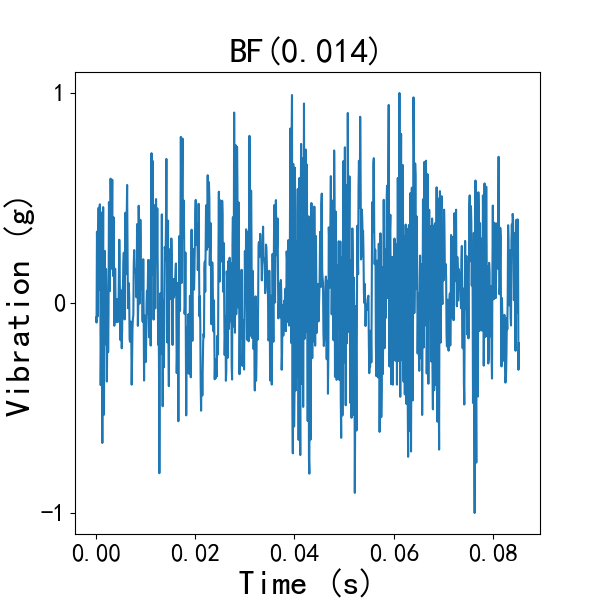
\includegraphics[width=0.28\linewidth]{class_5.png}
        \label{class_5}
    }
    \\ % 换行
    \subfloat[]{
        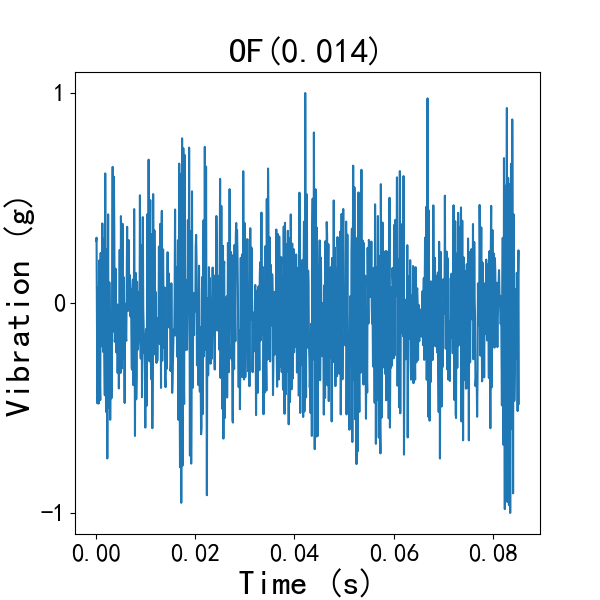
\includegraphics[width=0.28\linewidth]{class_6.png}
        \label{class_6}
    }
    \subfloat[]{
        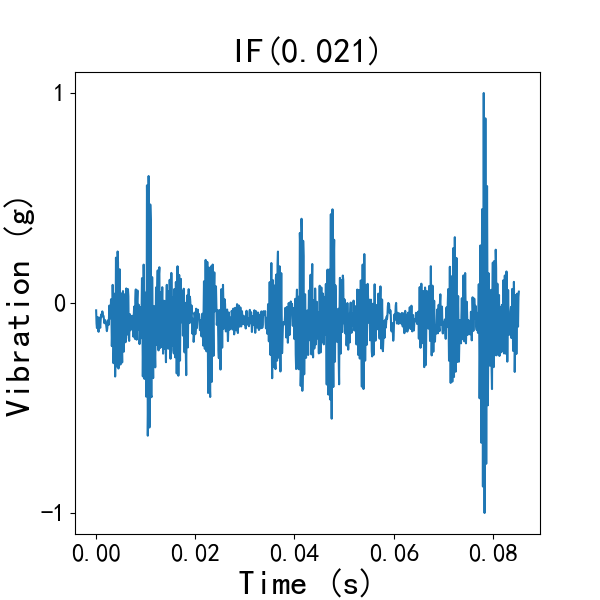
\includegraphics[width=0.28\linewidth]{class_7.png}
        \label{class_7}
    }
    \subfloat[]{
        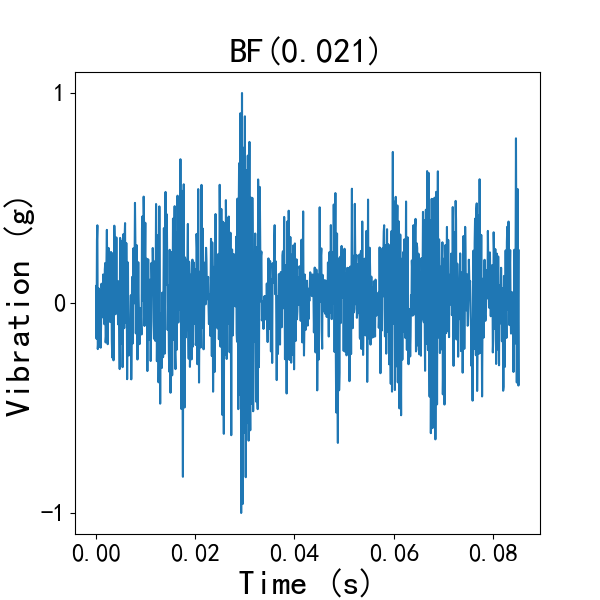
\includegraphics[width=0.28\linewidth]{class_8.png}
        \label{class_8}
    }
    \\ % 换行
    \subfloat[]{
        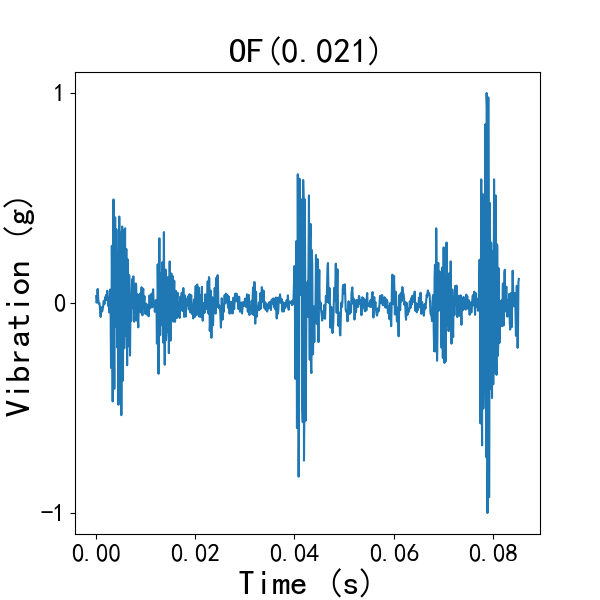
\includegraphics[width=0.28\linewidth]{class_9.png}
        \label{class_9}
    }

    \caption{每个类别的样本信号:\textbf{(a)} NC;\textbf{(b)} IF(0.007);\textbf{(c)} BF(0.007);\textbf{(d)} OF(0.007);\textbf{(e)} IF(0.014);\textbf{(f)} BF(0.014);\textbf{(g)} OF(0.014);\textbf{(h)} IF(0.021);\textbf{(i)} BF(0.021);\textbf{(j)} OF(0.021)。}
    \label{cwru_samples}
\end{figure}



\chapter{基于孪生网络对比学习的自监督预训练方法研究}
在本章,我们提出了一种基于孪生网络对比学习的自监督学习故障诊断框架。我们设计了一种新颖的数据增强策略搜索算法,并在\ref{sec:discuss_of_simsiam_module}小节中对数据增强模块在该框架中的必要性和设计方向进行了详细的理论分析和实验。

设计孪生网络的一个关键挑战是防止网络输出出现“坍塌”现象,即输出最终趋向于一个常数的平凡解。为了解决这一问题,本章首先介绍了简单的暹罗孪生网络框架,并结合实验与理论分析,探讨了各个模块在防止网络“坍塌”方面的作用。我们通过一系列实验证明了框架的有效性和鲁棒性,特别是在实际应用中如何通过合理设计避免模型的退化问题。
\section{模型整体架构及其模块设计}
\subsection{简单暹罗孪生网络}
\begin{figure}[h]
    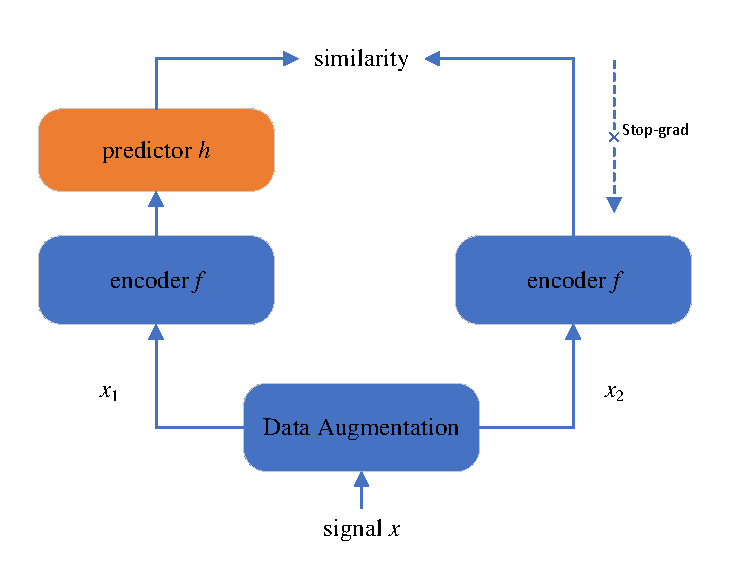
\includegraphics[width=12cm]{simsiam_arch.pdf}
    \caption{简单暹罗孪生网络}
    \label{simsiam_arch}
\end{figure}
简单暹罗孪生网络(SimSiam——Simple Siamese)\citing{chen2021exploring}架构(图\ref{simsiam_arch})将信号$x$中的两个随机增强视图$x_1$和$x_2$作为输入。这两个视图由编码器网络$f$处理,该网络由骨干网络(例如ResNet\citing{he2016deep})和投影MLP头部组成。编码器$f$在两个视图之间共享权重。预测MLP头部$h$转换一个视图的输出并将其与另一个视图进行匹配。将两个输出向量表示为$p_1 \triangleq h(f(x_1))$和$z_2 \triangleq f(x_2)$,我们最小化它们的负余弦相似度:
\begin{equation}
    \mathcal{D}(p_1, z_2) = -\frac{p_1}{\|p_1\|_2} \cdot \frac{z_2}{\|z_2\|_2}
    \label{eq:distance}
\end{equation}  
其中,$\|\cdot\|_2$ 是 $\ell_2$范数。定义对称损失函数
\begin{equation}
    \mathcal{L} = \frac{1}{2} \mathcal{D}(p_{1}, z_{2}) + \frac{1}{2} \mathcal{D}(p_{2}, z_{1})
\label{eq:cos_loss}
\end{equation}
该损失函数作用于单段信号,总损失值在计算所有信号的损失后取平均值。损失函数的最小值为-1。

方法中一个重要的组件是梯度停止(stop-grad)操作(图 1)。我们通过修改公式(\ref{eq:distance}) 来实现它:
\begin{equation}
    D(p_1, \text{stopgrad}(z_2))
\label{eq:stopgrad}
\end{equation}
这意味着在这一项中,\( z_2 \) 被视为常数。类似地,公式(\ref{eq:cos_loss}) 的实现形式为:
\begin{equation}
\mathcal{L} = \frac{1}{2} D(p_1, \text{stopgrad}(z_2)) + \frac{1}{2} D(p_2, \text{stopgrad}(z_1))
\label{eq:cos_loss_stopgrad}
\end{equation}
第一项中 \( x_2 \) 的编码器不会从 \( z_2 \) 接收梯度,但在第二项中会从 \( p_2 \) 接收梯度(反之亦然,对于 \( x_1 \) 也是如此)。即在这一项中,\( z_2 \) 被视为常数。

简单暹罗孪生网络的伪代码如表\ref{table:simsiam_code}所示。

\begin{table}
    \caption{简单暹罗孪生网络的伪代码,用Pytorch描述}
    \begin{tabular}{@{}l@{}} % 使用 @{} 去掉默认的左右边距,l 表示左对齐
    \toprule
    \multicolumn{1}{@{}l@{}}{\textbf{简单暹罗孪生网络Pytorch伪代码}} \\ % 左对齐文本
    \midrule
    \begin{lstlisting}[basicstyle=\ttfamily,frame=none]
#f: 骨干网络 + 投影 MLP
#h: 预测 MLP
for x in loader:  # 加载一个包含 n 个样本的小批量数据 x
    x1, x2 = aug(x), aug(x)  # 随机数据增强
    z1, z2 = f(x1), f(x2)  # 投影,形状为 n-by-d
    p1, p2 = h(z1), h(z2)  # 预测,形状为 n-by-d
    L = D(p1, z2)/2 + D(p2, z1)/2  # 损失函数

    L.backward()  # 反向传播
    update(f, h)  # SGD 更新

def D(p, z):  # 负余弦相似度
    z = z.detach()  # 停止梯度
    p = normalize(p, dim=1)  # 对 p 进行 L2 归一化
    z = normalize(z, dim=1)  # 对 z 进行 L2 归一化
    return -(p * z).sum(dim=1).mean()  # 计算负余弦相似度
    \end{lstlisting} \\
    \bottomrule
    \end{tabular}
    \label{table:simsiam_code}
\end{table}
\subsection{简单暹罗孪生故障诊断网络}
\begin{figure}[h]
    \centering
    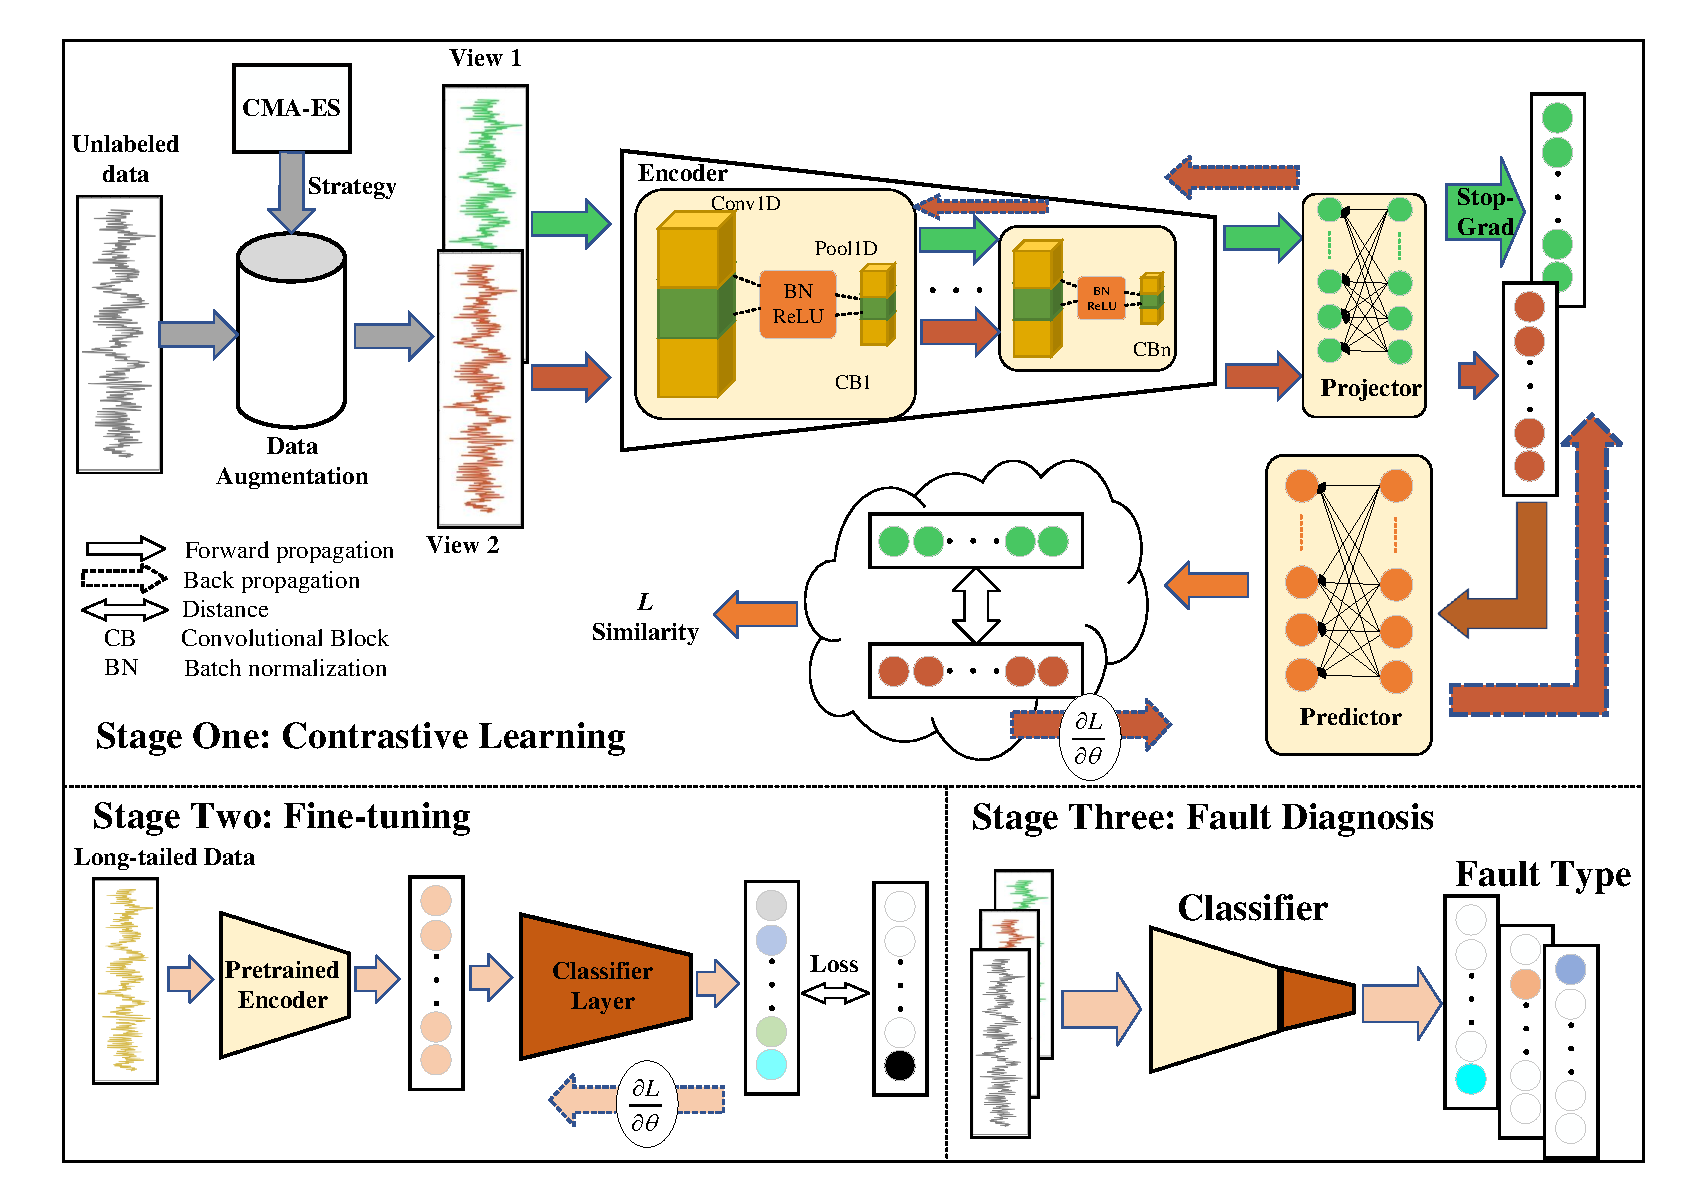
\includegraphics[width=16cm]{simsiam_net.pdf}
    \caption{简单暹罗孪生故障诊断网络}
    \label{simsiam_net}
\end{figure}
提出的用于故障诊断的简单暹罗孪生网络如图\ref{simsiam_net}所示,以下是架构的介绍。

1)\textbf{数据增强(Data Augmentations)}:
在对比表示学习算法中,数据增强(DA)起着至关重要的作用。网络的编码器(Encoder)能否成功地从振动信号中提取可区分的故障特征,依赖于为同一样本生成不同视图的质量。我们知道,面向图像的最新(SOTA)对比表示学习算法广泛使用多种数据增强方法,而针对序列数据的增强方法则相对较少。
此外,用于对比学习生成正样本对的增强方法必须满足一个条件,即加入样本的噪声不能改变其语义含义。同时,数据增强模块需要有效地带来多样化的特征空间分布来迫使编码器学习深层语义特征(根据\ref{sec:discuss_of_simsiam_module}节对数据增强的理论分析)。因此,我们选择了以下九种数据增强方法:

\begin{itemize}
    \item \textbf{掩码(Random Masked)}:用于遮盖输入数据的一部分,即随机挑选信号的某些部分用 0 替代,通常是在序列数据或图像数据中随机选择部分区域进行掩码处理。这有助于模型在训练时学会忽略一些无关信息,从而提高其鲁棒性。

    \item \textbf{添加高斯噪声(Adding Gaussian Noise)}:将高斯噪声添加到数据中的方法,常用于增强模型的鲁棒性。通过这种方式,模型在训练过程中能够适应噪声,并提升其在实际应用中的性能,尤其是在存在噪声的环境中。

    \item \textbf{相位扰动(Phase Perturbation)}:修改信号的频率域中的相位信息,而保持幅度不变来生成新的数据样本。这种方法保留了信号的整体结构,但引入了细微的扰动,用于提高模型的泛化能力。

    \item \textbf{块打乱(RandomChunkShuffle)}:将时间序列数据分割成多个块,然后随机打乱这些块的顺序。这样可以创建不同的序列变体,增加模型对数据变异的适应能力,同时保持整体的语义不变。

    \item \textbf{随机缩放(Random Scaled)}:对数据进行随机幅度缩放来增强数据的方法。通过改变数据的尺度,模型能够学习到不同幅度下的数据模式,从而提升其泛化能力。

    \item \textbf{随机绝对值(Random Abs)}:对数据应用绝对值操作,将负值转换为正值或去掉负号。这个方法帮助模型处理包含负值的情形,增强其鲁棒性。

    \item \textbf{竖直翻转(Random Vertical Flip)}:随机地将数据进行竖直翻转来创建新的样本。这对于一些对竖直方向变化不敏感的任务非常有效。

    \item \textbf{水平翻转(Random Horizontal Flip)}:随机将图像或数据进行水平翻转,生成新的样本。这种方法对于对称性较强的数据非常有效,能增强模型的鲁棒性。

    \item \textbf{时移(Time Shift)}:将数据在时间轴上平移一定的时间步长来生成新的样本。这种方法可以帮助模型学会适应时间序列数据中事件的变化位置,提升其对时间依赖的理解能力。
\end{itemize}

同一输入信号分别经过上述数据增强方法后的视图如图\ref{data_augmentation}所示。
\begin{figure}[h]
    \centering
    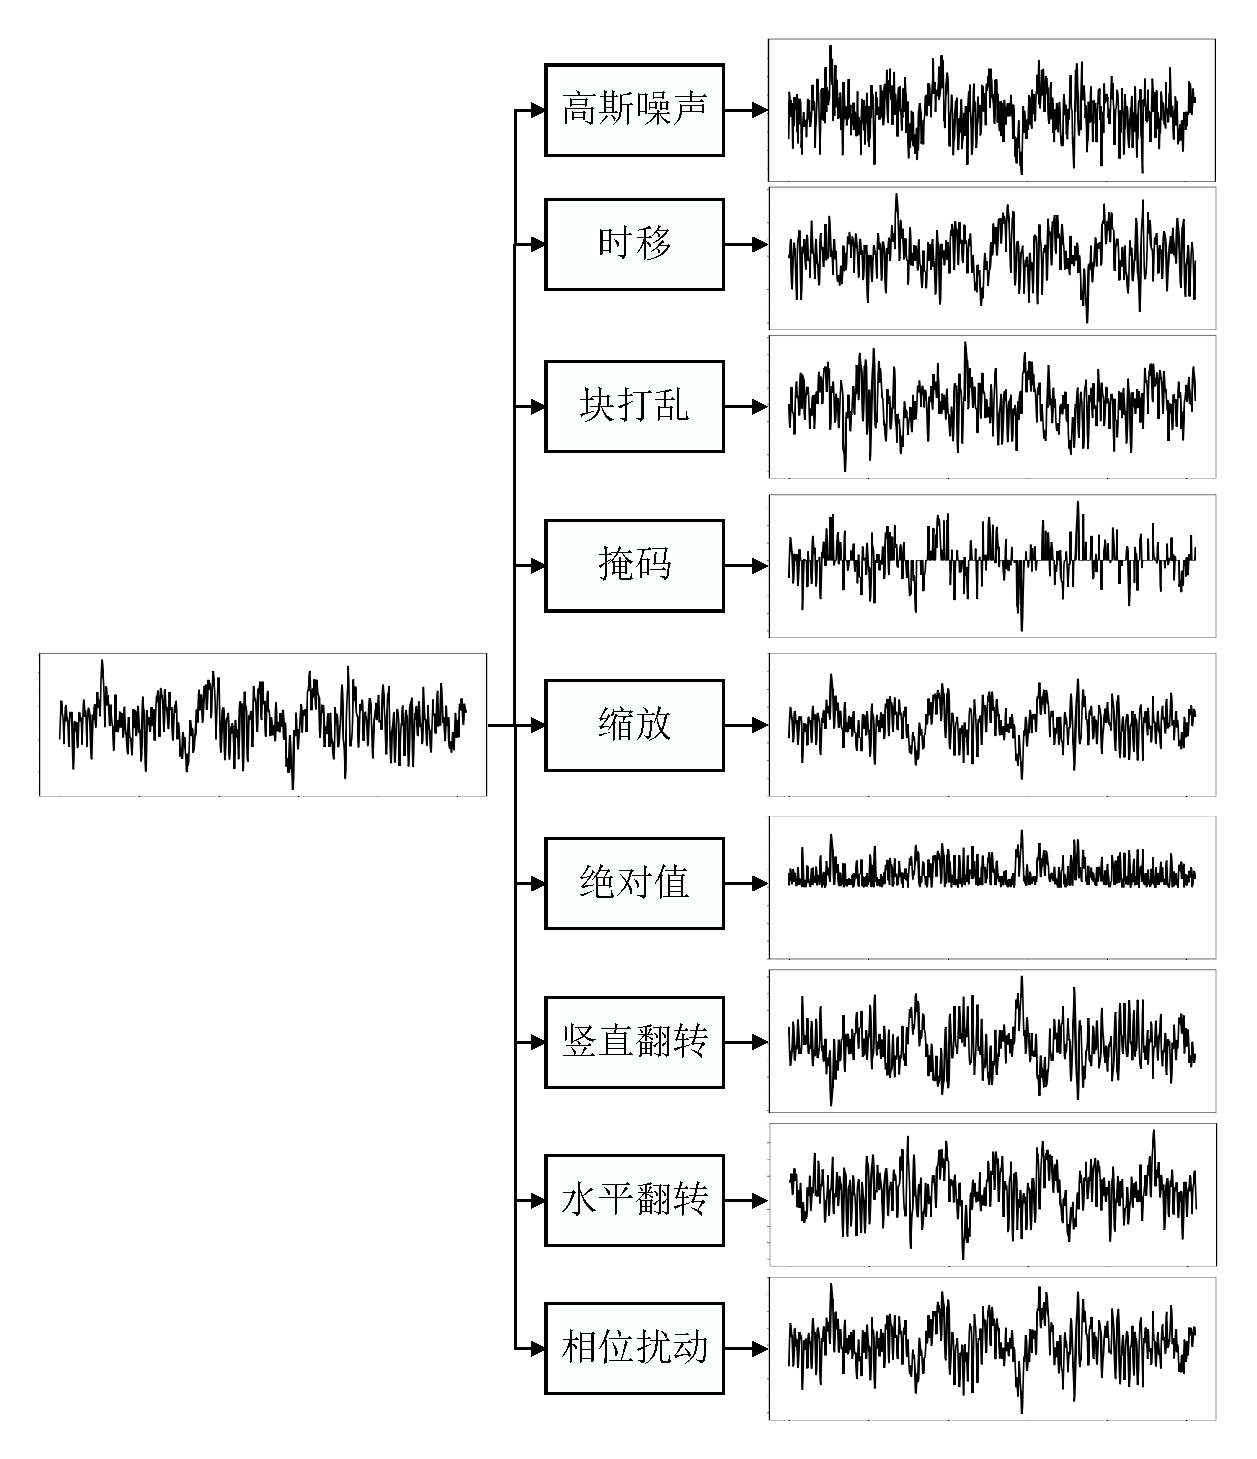
\includegraphics[width=10cm]{data_augmentation.pdf}
    \caption{数据增强示意图}
    \label{data_augmentation}
\end{figure}

2)\textbf{编码器(Encoder),预测器(Predictor)和分类器(Classifier)}:编码器是该算法中故障诊断的关键部分。我们主要使用其潜在编码来完成分类任务。由于简单暹罗网络是一个框架,我们可以根据需要构建编码器模型和预测器,其中预测器是一个相对简单的非线性函数。在第二阶段,需要在预训练的编码器后添加一个分类器层用于故障诊断,如图\ref{simsiam_net}所示。为了方便起见,我们使用多个常规的卷积神经网络(CNN)块来构建编码器,并使用全连接层来构建预测器和分类器。每个卷积块(CB)包括四个层:一个 1-D 卷积层\( f_{\text{BN}} \)、一个激活函数层 \( f_{\text{ReLU}} \),以及一个池化层 \( f_{\text{Pool}} \)。 方程(\ref{eq:CNN})展示了 1-D 卷积层的操作,其中输入的形状为 \( (N, C_{\text{in}}, L) \),输出的形状为 \( (N, C_{\text{out}}, L_{\text{out}}) \),其中 \( N \) 是样本的数量,\( C \) 表示通道数,\( L \) 表示数据的长度。
\begin{equation}
    \begin{aligned}
    \operatorname{out}(N_i, C_{\mathrm{out}_j}) &= \operatorname{bias}(C_{\mathrm{out}_j}) + \sum_{k=0}^{C_{\mathrm{in}}-1} \operatorname{weight}(C_{\mathrm{out}_j}, k) \otimes \operatorname{input}(N_i, k).
    \end{aligned}
    \label{eq:CNN}
    \end{equation}
BN 层 \( f_{\text{BN}} \) 用于加速训练过程并减少由于层输入分布不同而导致的内部协变量偏移(ICS)的影响 \citing{ioffe2015batch},当模型较深时,这种影响尤为严重。公式(\ref{eq:BN})展示了批归一化的过程。
\begin{equation}
    f_{\text{BN}}(x_i, \mathbf{x}) = \gamma \frac{x_i - \mathbb{E}(\mathbf{x})}{\sqrt{\sigma(\mathbf{x})^2 + \epsilon}} + \beta
\label{eq:BN}
\end{equation}    
\begin{equation}
\mathbb{E}(\mathbf{x}) = \frac{1}{N}\sum_{i=1}^N x_i
\label{eq:exp_BN}
\end{equation}
\begin{equation}
\sigma(\mathbf{x}) = \sqrt{\frac{1}{N}\sum_{i=1}^N (x_i - \mathbb{E}(\mathbf{x}))^2}
\label{eq:sigma_BN}
\end{equation}
其中 \( x \) 是整个小批量(mini batch)的向量,批量大小为 \( N \),\( x_i \) 表示小批量中的第 \( i \) 个样本。  
\( \mathbb{E}(x) \) 和 \( \sigma(x) \) 分别表示向量批量的均值和方差,如公式 (\ref{eq:exp_BN}) 和 (\ref{eq:sigma_BN}) 所示。\( \epsilon \) 是一个超参数,通常设置为 \( 10^{-5} \),而 \( \gamma \) 和 \( \beta \) 分别是缩放因子和偏移因子,它们是可学习的参数,初始值分别设置为 1 和 0。

激活层 \( f_{\text{ReLU}} \) 可以表示为公式 (\ref{eq:relu}):
\begin{equation}
    f_{\text{ReLU}} = \max(0, x)
    \label{eq:relu}
\end{equation}

\( x_i^{(n)} \) 表示通过第 \( n \) 个卷积块(CB)的第 \( i \) 个输出向量,可以用公式 (\ref{eq:output_of_encoder}) 表示:
\begin{equation}
    \begin{aligned}
    x_i^{(n)} = f_{\text{Pool}}\bigl\{f_{\text{ReLU}}\bigl[f_{BN}\Bigl(f_{\text{conv}}\bigl(\mathbf{x}^{(n-1)}\bigr), f_{\text{conv}}\Bigl(x_i^{(n-1)}\Bigr)\Bigr)\bigr]\bigr\}
    \end{aligned}
    \label{eq:output_of_encoder}
\end{equation}

3)\textbf{优化器(Optimizer)}:模型的训练不需要使用大批量优化器,例如分层自适应速率缩放(LARS)\citing{you2017large},因为所提出的方法可以在典型批量大小下工作,而不依赖于大批量训练。我们使用 SGD 优化器训练模型。网络参数通过公式 (\ref{eq:SGD}) 更新。
\begin{equation}
    \theta_{l+1} = \theta_l - \eta_l \cdot \nabla_{\theta} \mathcal{L}(\mathbf{x}; \theta_l)
\label{eq:SGD}
\end{equation}
其中 \( \theta_t \) 表示时间 \( t \) 时的可学习参数,\( \eta_t \) 表示时间 \( t \) 时的学习率,\( L(\cdot) \) 表示损失函数。

4)\textbf{微调(Fine-tuning)}:在对比学习阶段完成后,我们从模型中取出训练好的编码器 \( f \),并将其与一个多层感知器(MLP)模块连接,我们用带标签的数据微调构建一个完整的分类器用于故障诊断任务,从而使模型获得分类能力。以准确率为性能指标,如公式 (\ref{eq:acc}):
\begin{equation}
    \text{Accuracy} = \frac{TN + TP}{TN + TP + FP + FN}
    \label{eq:acc}
\end{equation}
其中,\( TN \) 表示真阴性,即被正确预测为阴性的阴性样本数量。真阳性(\( TP \))表示被模型正确判断为阳性的阳性样本数量。假阳性(\( FP \))表示被错误分类为阳性的阴性样本数量。假阴性(\( FN \))表示被错误分类为阴性的阳性样本数量。  

当验证集的样本均匀采样后(本研究采用此方法),准确率等于宏平均召回率(Macro-Averaged Recall)。宏平均召回率是对每个类别单独计算召回率,然后取平均值:
\begin{equation}
    \text{Macro-Recall} = \frac{1}{C} \sum_{i=1}^{C} \frac{TP_i}{TP_i + FN_i}
    \label{eq:macro_recall}
\end{equation}
其中,\( C \) 是类别的总数,\( TP_i \) 和 \( FN_i \) 分别是第 \( i \) 类的真正例和假负例。




5)\textbf{故障诊断(Fault Diagnosis)}:在完成微调后,即可将模型应用于真实输入信号的故障诊断,以预测故障类别。
\begin{figure}[h]
    \centering
    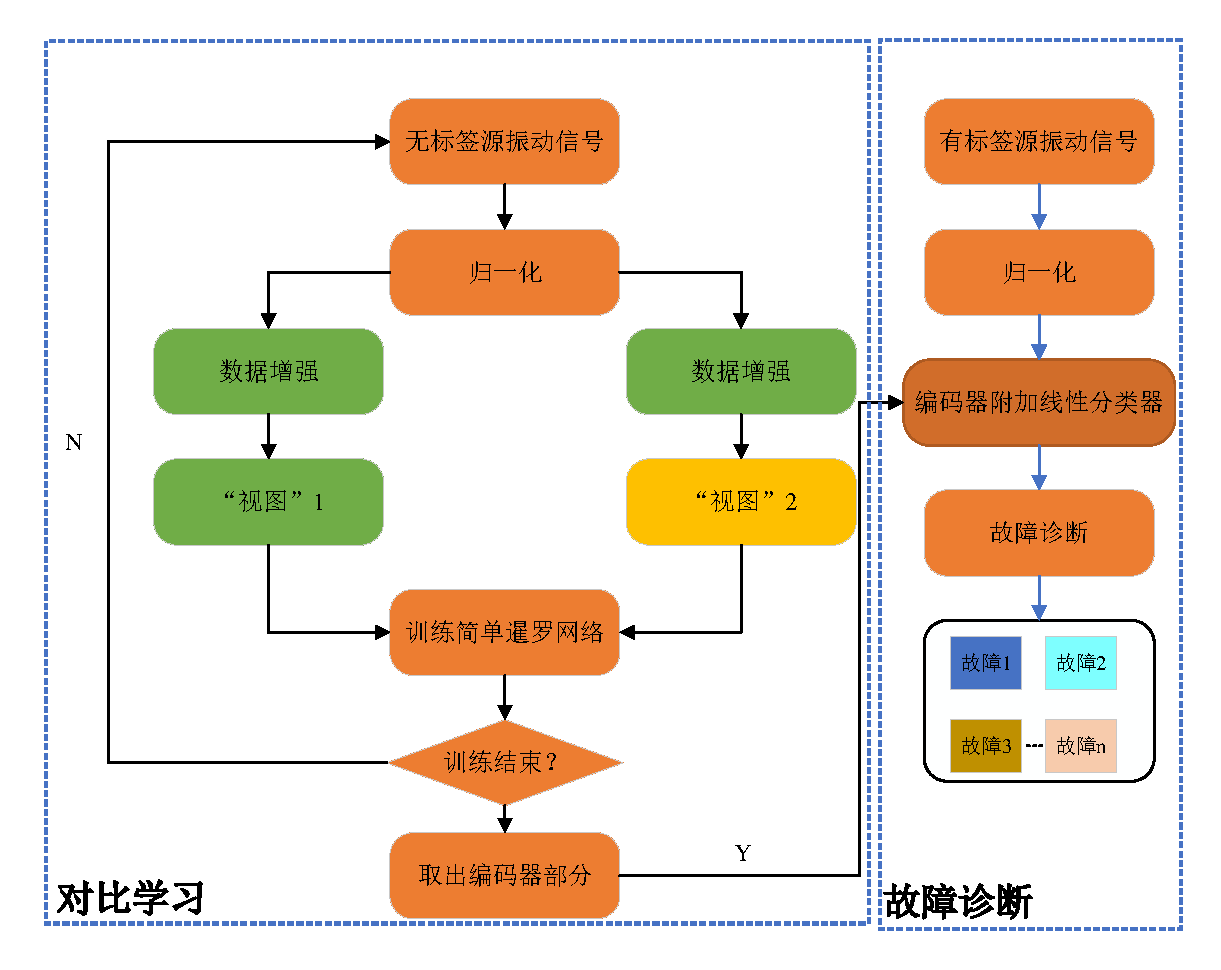
\includegraphics[width=14cm]{simsiam_fault_diag_procedure.pdf}
    \caption{简单暹罗孪生故障诊断网络的训练流程图}
    \label{simsiam_fault_diag_procedure}
\end{figure}
简单暹罗孪生故障诊断网络的训练过程如图\ref{simsiam_fault_diag_procedure}所示。首先,我们需要对所有未标记的振动样本进行归一化预处理,并使用数据增强方法生成输入样本的两个不同视图作为正样本对。我们将正样本对输入模型,然后按照算法表\ref{table:simsiam_code}所示的流程训练模型。训练过程完成后,我们取出编码器,在其最后一层后附加一个线性分类层,并使用标记样本对模型进行微调。线性分类层也可以用其他分类器(如 K 近邻(KNN)和支持向量机(SVM))替换。

\subsection{基于CMA-ES优化器的最优数据增强策略搜索算法}
\begin{figure}[h]
    \centering
    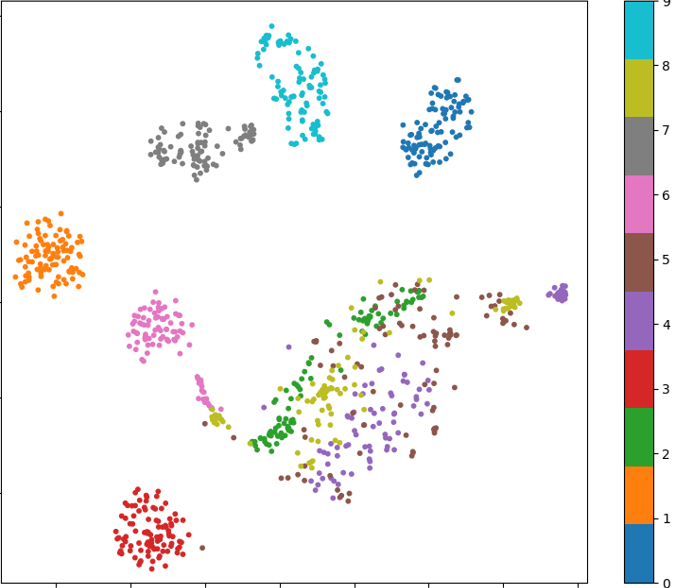
\includegraphics[width=6cm]{simsiam_no_cma_tsne.png}
    \caption{基于人工设定数据增强策略的SimSiam特征t-SNE图}
    \label{simsiam_no_cma_tsne}
\end{figure}
简单暹罗孪生网络(SimSiam)的一个显著问题是可能出现所有输出“坍塌”为常数的平凡解。SimSiam通过数据增强生成两个视图,并直接最大化同一输入的两个视图之间的相似性,而不依赖于负样本对。因此,其性能在很大程度上依赖于数据增强策略的质量(不改变原语义的同时丰富特征空间)。然而,人工设计数据增强策略不仅耗时耗力,还难以获得最优方案。如图\ref{simsiam_no_cma_tsne}所示,基于人工设定数据增强策略训练的SimSiam网络在特征提取效果上存在明显不足,该策略未能有效提取样本间的区分性特征,导致相对大一部分类别的样本特征“糅杂”在一起。该节提出了基于CMA-ES优化器的最优数据增强策略搜索算法,CMA-ES(Covariance Matrix Adaptation Evolution Strategy,协方差矩阵自适应进化策略)是一种用于连续优化问题的进化算法。它是一种基于种群的优化方法,通过自适应调整协方差矩阵来指导搜索方向,从而在高维空间中高效地找到全局最优解。CMA-ES 在解决非线性、非凸、高维优化问题时表现出色,广泛应用于机器学习、工程优化和科学研究中。CMA-ES 的更新规则如下:

1. 采样新解:
\begin{equation}
\mathbf{x}_k^{(g+1)} = \mathbf{m}^{(g)} + \sigma^{(g)} \cdot \mathcal{N}(0, \mathbf{C}^{(g)})
\label{eq:sample}
\end{equation}
其中:
\begin{itemize}
    \item \(\mathbf{x}_k^{(g+1)}\) 是第 \(g+1\) 代中的第 \(k\) 个候选解,
    \item \(\mathbf{m}^{(g)}\) 是第 \(g\) 代的均值向量,
    \item \(\sigma^{(g)}\) 是第 \(g\) 代的步长,
    \item \(\mathbf{C}^{(g)}\) 是第 \(g\) 代的协方差矩阵,
    \item \(\mathcal{N}(0, \mathbf{C}^{(g)})\) 是从多元正态分布中采样的随机向量。
\end{itemize}

2. 更新均值:
\begin{equation}
\mathbf{m}^{(g+1)} = \sum_{i=1}^{\mu} w_i \mathbf{x}_{i:\lambda}^{(g+1)}
\label{eq:mean_update}
\end{equation}
其中:
\begin{itemize}
    \item \(\mu\) 是选择的父代数量,
    \item \(w_i\) 是权重系数,
    \item \(\mathbf{x}_{i:\lambda}^{(g+1)}\) 是第 \(g+1\) 代中适应度排名前 \(\mu\) 的候选解。
\end{itemize}

3. 更新协方差矩阵:
\begin{equation}
\mathbf{C}^{(g+1)} = (1 - c_1 - c_\mu) \mathbf{C}^{(g)} + c_1 \mathbf{p}_c^{(g+1)} (\mathbf{p}_c^{(g+1)})^\top + c_\mu \sum_{i=1}^{\mu} w_i \mathbf{y}_{i:\lambda}^{(g+1)} (\mathbf{y}_{i:\lambda}^{(g+1)})^\top
\label{eq:covariance_update}
\end{equation}
其中:
\begin{itemize}
    \item \(c_1\) 和 \(c_\mu\) 是学习率,
    \item \(\mathbf{p}_c^{(g+1)}\) 是进化路径,
    \item \(\mathbf{y}_{i:\lambda}^{(g+1)} = (\mathbf{x}_{i:\lambda}^{(g+1)} - \mathbf{m}^{(g)}) / \sigma^{(g)}\)。
\end{itemize}

4. 更新步长:
\begin{equation}
\sigma^{(g+1)} = \sigma^{(g)} \exp\left(\frac{c_\sigma}{d_\sigma} \left(\frac{\|\mathbf{p}_\sigma^{(g+1)}\|}{\mathbb{E}[\|\mathcal{N}(0, \mathbf{I})\|]} - 1\right)\right)
\label{eq:stepsize_update}
\end{equation}
其中:
\begin{itemize}
    \item \(c_\sigma\) 是步长学习率,
    \item \(d_\sigma\) 是阻尼系数,
    \item \(\mathbf{p}_\sigma^{(g+1)}\) 是步长进化路径,
    \item \(\mathbb{E}[\|\mathcal{N}(0, \mathbf{I})\|]\) 是标准正态分布向量的期望范数。
\end{itemize}

我们将寻找最佳数据增强策略的问题形式化为一个搜索问题(见图 \ref{CMA-ES})。我们的方法由两个组件组成:搜索算法和搜索空间。在高层次上,搜索算法(实现为CMA-ES)采样一个数据增强策略 \( S \),该策略包含有关使用哪种图像处理操作、每批次中使用该操作的概率以及操作幅度的信息。我们方法的关键在于,策略 \( S \) 将用于训练具有固定架构的神经网络,其验证准确率 \( R \) 将返回以评估适应度。
\begin{figure}[h]
    \centering
    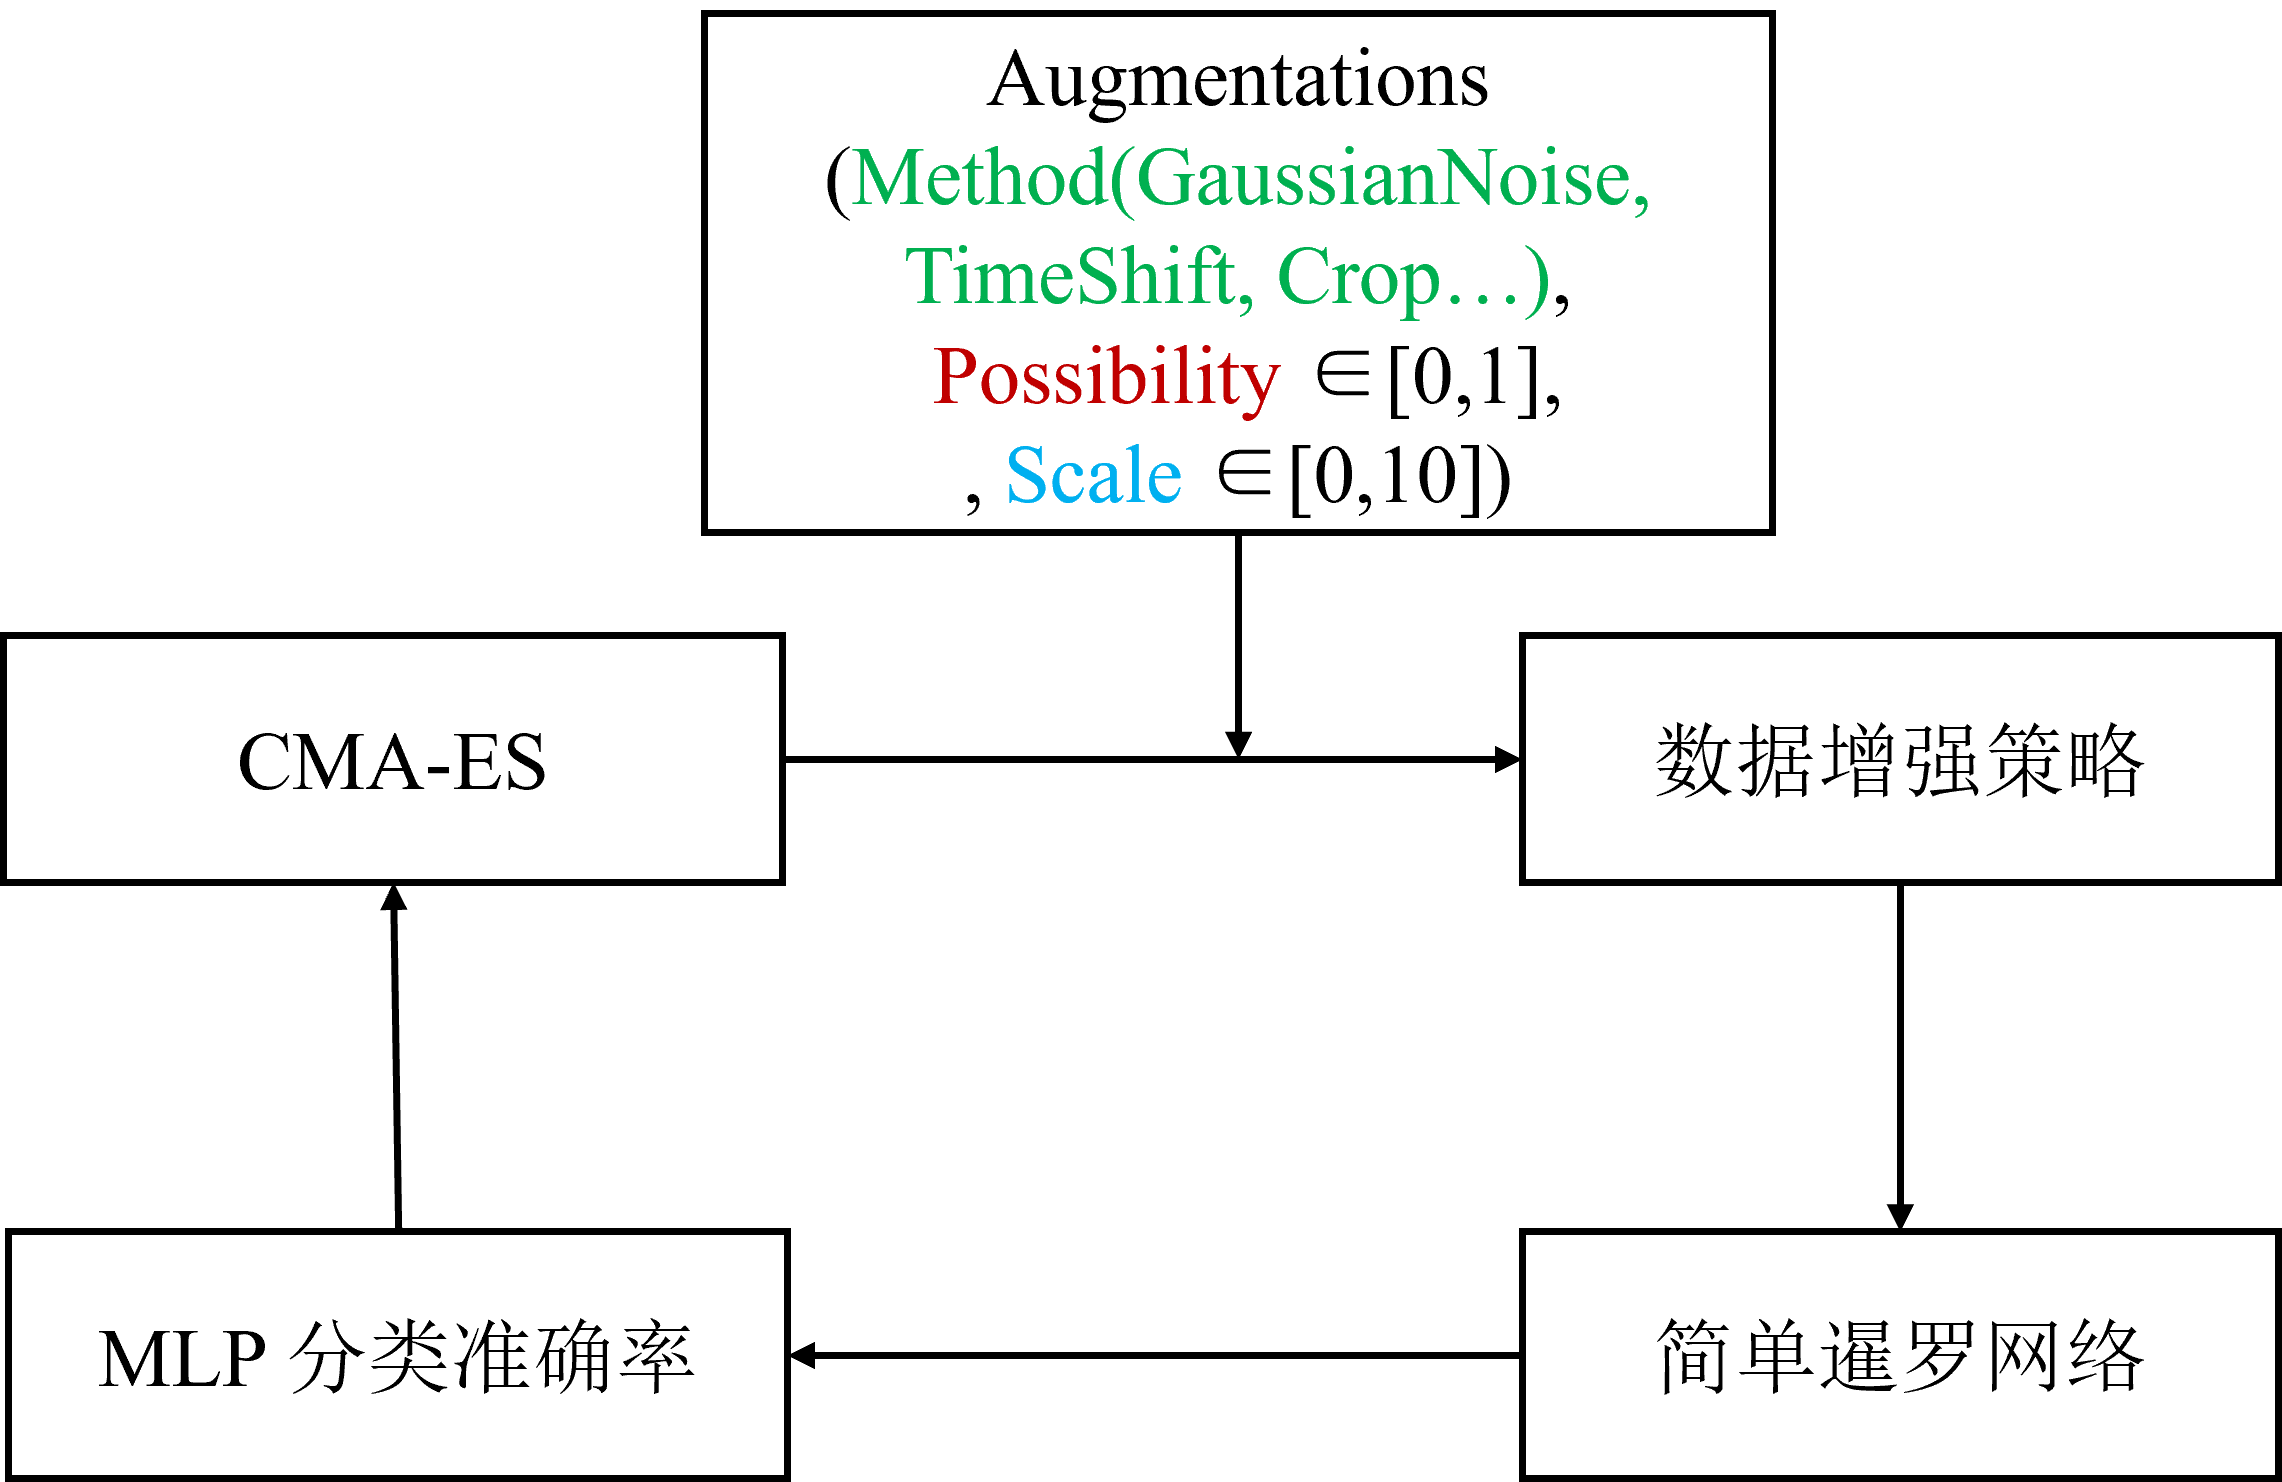
\includegraphics[width=8cm]{CMA-ES.png}
    \caption{使用CMA-ES搜索最优的数据增强策略框架概览}
    \label{CMA-ES}
\end{figure}
搜索空间细节:在我们的搜索空间中,一个策略由 8 个信号数据增强子策略组成,如图\ref{data_augmentation}所示。此外,每个操作还关联两个超参数:
\begin{itemize}
    \item 1) 应用操作的概率\(\in [0,1]\),
    \item 2) 操作的幅度映射后\(\in [0,10]\)。
\end{itemize}
映射为线性变换,如变量\(x \in [a,b]\)到\(y \in [0,10]\)的变换为
\begin{equation}
    y = \frac{10(x - a)}{b - a}
    \end{equation}
以下介绍各个数据增强子策略幅度的表示:
\begin{itemize}
    \item \textbf{掩码(Random Masked)}:随机选取100个不重叠的大小为$s$的子区间,将其置0。$s$作为增强幅度由\([1,5]\)映射为\([0,10]\)。

    \item \textbf{添加高斯噪声(Adding Gaussian Noise)}:将高斯噪声的信噪比SNR作为增强幅度,由\([2,6]\)映射为\([0,10]\)。

    \item \textbf{相位扰动(Phase Perturbation)}:相位扰动服从均匀分布$\text{U}(-perturb_{\text{max}}, perturb_{\text{max}})$,$perturb_{\text{max}}$作为增强幅度由\([0.1,0.5]\)映射为\([0,10]\)。

    \item \textbf{块打乱(RandomChunkShuffle)}:将时间序列数据分割成大小均匀的$s$个块,然后随机打乱这些块的顺序。$s$作为增强幅度由\([10,100]\)映射为\([0,10]\)。

    \item \textbf{随机缩放(Random Scaled)}:缩放的幅度服从均匀分布$\text{U}(1.0-scale, 1.0+scale)$。$scale$作为增强幅度由\([0.05,0.6]\)映射为\([0,10]\)。

    \item \textbf{随机绝对值(Random Abs)}:无幅度值。

    \item \textbf{竖直翻转(Random Vertical Flip)}:无幅度值。

    \item \textbf{水平翻转(Random Horizontal Flip)}:无幅度值。
    
\end{itemize}
则CMA-ES优化器求解的问题可以描述为 
\begin{equation}
    \arg\max_{\mathbf{p}, \mathbf{s}} \text{Accuracy}(\mathbf{p}, \mathbf{s}, \text{SimSiam-Net})
\end{equation}
其中,\(\mathbf{p}\) 和 \(\mathbf{s}\) 为求解的参数,分别满足 \(p_i \in [0, 1]\) 和 \(s_i \in [0, 10]\),Accuracy为简单暹罗网络验证的准确率。

\section{实验与分析}
为了验证所提出方法的有效性,我们选择了三种不同的轴承故障数据进行实验。它们分别是 CWRU 数据集、SQ 数据集和 PB 数据集。此外,为了证明所提出方法的优越性,我们选择了几种流行的方法作为对比方法,这些方法可以分为两类。一类是传统的机器学习算法,另一类是当前基于深度学习的智能方法。对比方法如下所示。
\begin{enumerate}
    \item \textbf{SVM\citing{ziani2017bearing}}:多类 SVM 是一种强大且多功能的机器学习模型,能够执行线性或非线性分类任务。首先,我们将计算原始数据的 16 个时域指标(均值、平方根、偏度等),并将它们作为 SVM 分类器的输入。

    \item \textbf{CNN\citing{eren2019generic}}:CNN 是一种监督学习方法。在这里,CNN 的网络架构与所提出方法的编码器 \(f\) 相同。

    \item \textbf{BYOL\citing{grill2020bootstrap}}:BYOL(Bootstrap Your Own Latent)是一种基于自监督学习的表示学习方法。与传统的对比学习方法不同,BYOL 不依赖于负样本对进行训练,而是通过最大化正样本对之间的相似度来学习图像表示。该方法使用两个神经网络块,其中一个作为在线网络(online network),另一个作为目标网络(target network)。两个网络共享相同的编码器 \(f\),但参数更新的方式不同:在线网络的参数通过反向传播进行更新,而目标网络的参数则通过指数滑动平均(EMA)进行更新。编码器 \(f\) 和数据增强方法与所提出方法相同。
    
    \item \textbf{SimCLR\citing{chen2020simple}}:SimCLR 是一种基于对比学习的自监督表示学习方法,它通过最大化不同视图之间的相似度来学习图像表示。该方法使用一个编码器 \(f\),通常是一个卷积神经网络(CNN),并通过数据增强技术生成不同的图像视图。SimCLR 的训练目标是通过最大化正样本对的相似度并最小化负样本对的相似度,来优化表示学习的质量。该方法的关键创新是引入了基于温度缩放的对比损失函数,进而提升了模型的表达能力。编码器 \(f\) 和数据增强方法与所提出方法相同。

\end{enumerate}
\subsection{简单暹罗孪生网络实现细节}
由于简单暹罗网络是一个框架,我们可以根据需要构建编码器模型和预测器,以下介绍本文构建的简单暹罗网络框架的细节。
\begin{itemize}
    \item \textbf{Encoder}:堆叠了十个 CNN 块作为编码器,其中卷积层的核大小设置为 3,填充设置为 1,步幅设置为 1,隐藏层采用 256 个核。
    
    \item \textbf{Predictor}:我们使用两个线性全连接层构建预测器,分别具有 \( 256 \times 512 \) 和 \( 512 \times 256 \) 个神经元。我们在它们之间放置了一个批归一化层和一个修正线性单元(ReLU)层。

    \item \textbf{Classifier}:至于分类器层,我们也部署了两个线性全连接层,分别具有 \( 256 \times 256 \) 和 \( 256 \times \text{num\_class} \) 个神经元,其中 \(\text{num\_class}\) 表示故障类别的数量。在两个线性层之间也放置了一个批归一化层和一个 ReLU 层。

    \item \textbf{Optimizer}:
        优化器为 SGD 优化器,其学习率初始设置为 \( 0.05 \times \frac{\text{BatchSize}}{256} \),学习率采用余弦衰减调度。余弦衰减调度的公式为:
        \[
        \eta_t = \eta_{\text{min}} + \frac{1}{2} (\eta_{\text{max}} - \eta_{\text{min}}) \left(1 + \cos\left(\frac{t \pi}{T}\right)\right)
        \]
        其中:
        \begin{itemize}
            \item \(\eta_t\) 是第 \(t\) 步的学习率,
            \item \(\eta_{\text{max}}\) 是初始学习率(最大学习率),
            \item \(\eta_{\text{min}}\) 是最小学习率,
            \item \(t\) 是当前训练步数,
            \item \(T\) 是总训练步数(衰减周期),
            \item \(\cos\) 是余弦函数。
        \end{itemize}
        权重衰减为 0.0001,SGD 动量为 0.9。

    \item \textbf{损失函数}:对比学习预训练阶段的损失函数为余弦相似度见式(\ref{eq:distance}),微调阶段的损失函数为交叉熵损失函数(Cross-Entropy Loss Function)。对于多分类问题,交叉熵损失函数表示为
    \begin{equation}
        \mathcal{L}_{\text{CE}} = -\sum_{i=1}^{C} y_i \log(\hat{y}_i)
        \end{equation}        
        其中:
        \begin{itemize}
            \item \( C \) 是类别数量,
            \item \( y_i \) 是真实标签的 one-hot 编码(第 \( i \) 类的真实概率),
            \item \( \hat{y}_i \) 是模型预测的第 \( i \) 类的概率。
        \end{itemize}

    \item \textbf{长尾分布数据集模拟构造}:模拟构建长尾分布数据集流程如图\ref{pareto}所示。设定不平衡因子 \(\beta = x_{\text{max}} / x_{\text{min}}\) 为数据集中样本数量最多的类与样本数量最少的类的数量之比。帕累托分布的概率密度函数为 \(p(x) = \frac{\alpha x_{\text{min}}^{\alpha}}{x^{\alpha+1}}\),令$x_{\text{min}} = 1$,则\(p(x) = \frac{\alpha}{x^{\alpha+1}}\)。以不平衡因子构建服从帕累托分布的长尾分布数据集,不同不平衡因子的帕累托分布概率密度函数如图\ref{paerto_fig_beta}所示,可以看到当最大类与最小类样本数的比值 \(\beta\) 增大时,帕累托分布的形状参数 \(\alpha\) 也随之增大。这表明分布的头部类别占比提高,而尾部类别占比显著降低,长尾效应越发显著。下面将介绍形状参数 \(\alpha\) 的求解方法,以及各类别样本占比的计算步骤。

    \begin{figure}[h]
        \centering
        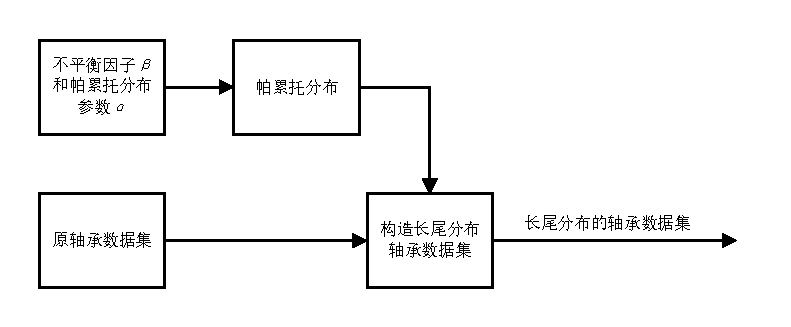
\includegraphics[width=12cm]{pareto.pdf}
        \caption{基于帕累托分布构造长尾分布的轴承数据集流程图}
        \label{pareto}
    \end{figure}

    \begin{figure}[h]
        \centering
        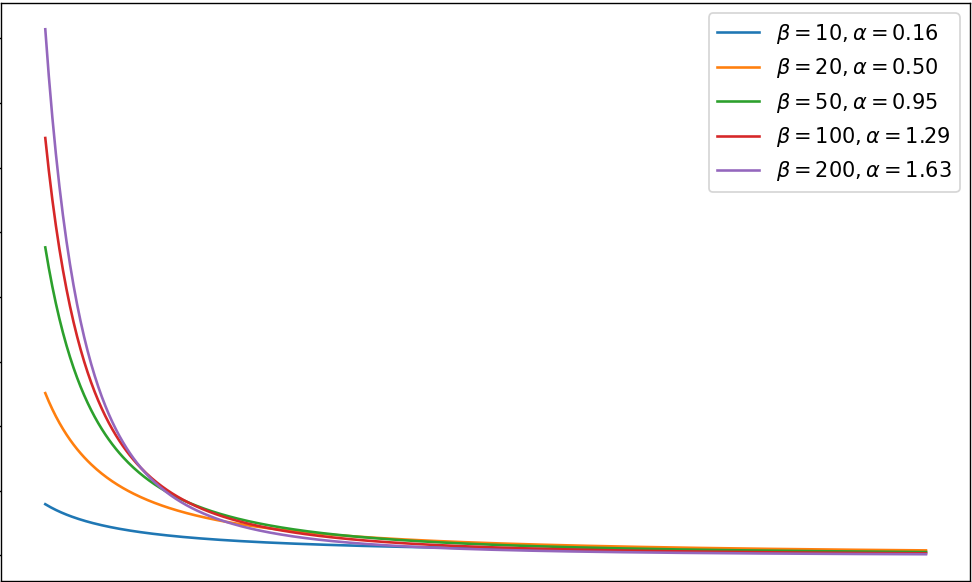
\includegraphics[width=12cm]{paerto_fig_beta.png}
        \caption{不同$\beta$的帕累托分布概率密度图}
        \label{paerto_fig_beta}
    \end{figure}

    已知帕累托分布的累积分布函数为:
    \begin{equation}
    F(x) = 1 - x^{-\alpha}, \quad x > 1
    \end{equation}

    每类的概率定义为:
    \begin{equation}
    P(n \leq x < n+1) = F(n+1) - F(n) = n^{-\alpha} - (n+1)^{-\alpha}
    \end{equation}

    设最大类与最小类的样本数比值为 $\beta$,则有以下关系式:
    \begin{equation}
    \beta = \frac{P(1 \leq x < 2)}{P(n \leq x < n+1)} = \frac{1 - 2^{-\alpha}}{n^{-\alpha} - (n+1)^{-\alpha}}
    \end{equation}

    目标是:
    \begin{enumerate}
        \item 根据给定的 $\beta$ 和类别总数 $n$,求解形状参数 $\alpha$。
        \item 计算每类的样本占比 $P(n \leq x < n+1)$。
        \item 将所有类别的概率归一化,使其和为 1。
    \end{enumerate}

    具体步骤:

    \begin{enumerate}
        \item \textbf{求解 $\alpha$} \\
        根据 $\beta$ 的定义,解以下非线性方程以确定 $\alpha$:
        \begin{equation}
        \beta = \frac{1 - 2^{-\alpha}}{n^{-\alpha} - (n+1)^{-\alpha}}
        \end{equation}
        该方程一般无解析解,可以通过数值方法(如 Newton-Raphson 或其他优化算法)求解。

        \item \textbf{计算每类的概率} \\
        每类的概率可以通过以下公式计算:
        \begin{equation}
        P(n \leq x < n+1) = n^{-\alpha} - (n+1)^{-\alpha}, \quad n = 1, 2, \dots, N
        \end{equation}

        \item \textbf{概率归一化} \\
        将所有类别的概率归一化,计算归一化后的概率:
        \begin{equation}
        P_{\text{norm}}(n \leq x < n+1) = \frac{P(n \leq x < n+1)}{\sum_{k=1}^N P(k \leq x < k+1)}
        \label{pareto_sample}
        \end{equation}
        其中 $N$ 为类别总数,归一化后各类别的样本占比之和为 1:
        \begin{equation}
        \sum_{n=1}^N P_{\text{norm}}(n \leq x < n+1) = 1
        \end{equation}
    \end{enumerate}
    \item \textbf{数据细节}:
      每个样本包含 \textbf{1024} 个数据点。
      训练过程分为两个阶段:
      \begin{itemize}
          \item 在\textbf{第一阶段},我们随机选择每个故障类别的 \textbf{100} 个无标签样本进行模型训练,训练总计 \textbf{500} 个周期。
          \item 在\textbf{第二阶段},我们根据式(\ref{pareto_sample})构造服从 \textbf{帕累托分布} 的长尾分布有标签样本,以此微调模型,微调总计 \textbf{50} 个周期。
      \end{itemize}
      在整个训练过程中,每个输入模型的 mini-batch 大小设定为 \textbf{64}。
      
      \item \textbf{性能评估}:  
      测试集由每个故障类别均匀地随机选取 \textbf{100} 个样本组成。需要注意的是,微调过程中使用的子集与测试集完全独立。  
      性能评估由以下几个指标组成:

      \begin{itemize}
          \item \textbf{验证集准确率}:在验证集上评估模型的分类准确率,以衡量模型的泛化能力。该指标表示了模型对未知数据的分类能力。计算公式如式(\ref{eq:acc})。
          \item \textbf{t-SNE特征提取可视化}:使用t-SNE(t-分布随机邻居嵌入,t-Distributed Stochastic Neighbor Embedding)方法将高维特征降维至二维空间进行可视化分析,直观展示不同类别之间的聚类情况。该方法有助于分析模型对不同故障类别的区分能力。t-SNE 通过以下三个步骤来进行降维:

        \begin{enumerate}
            \item \textbf{计算高维相似度}:t-SNE 首先计算每对数据点之间的相似度。在高维空间中,对于任意两点 \(x_i\) 和 \(x_j\),其相似度通过条件概率 \(p_{ij}\) 表示,计算公式为:
            
            \begin{equation}
            p_{ij} = \frac{\exp\left( -\frac{\|x_i - x_j\|^2}{2\sigma_i^2} \right)}{\sum_{j \neq i} \exp\left( -\frac{\|x_i - x_j\|^2}{2\sigma_i^2} \right)}
            \end{equation}
            
            其中,\(\|x_i - x_j\|\) 表示高维空间中两点之间的欧氏距离,\(\sigma_i\) 是与点 \(x_i\) 相关的局部尺度参数,反映了该点的邻域大小。通过这种方式,t-SNE 保证了高维空间中相邻的数据点具有较高的相似度。
            
            \item \textbf{映射到低维空间}:接着,t-SNE 将数据映射到低维空间中,通常是二维或三维。在低维空间中,t-SNE 使用 t-分布(Student's t-distribution)来计算数据点之间的相似度,公式为:
            
            \begin{equation}
            q_{ij} = \frac{\left( 1 + \|y_i - y_j\|^2 \right)^{-1}}{\sum_{j \neq i} \left( 1 + \|y_i - y_j\|^2 \right)^{-1}}
            \end{equation}
            
            其中,\(y_i\) 和 \(y_j\) 是低维空间中的数据点,\(\|y_i - y_j\|\) 是它们之间的欧氏距离。t-分布的重尾特性使得它能够更加有效地处理聚类之间的距离,同时避免了在低维空间中过度拥挤的现象。
            
            \item \textbf{最小化KL散度}:t-SNE 的目标是最小化高维空间和低维空间中数据点相似度分布的差异。为此,t-SNE 通过最小化 Kullback-Leibler(KL)散度来优化模型的映射过程,KL 散度的计算公式为:
            
            \begin{equation}
            \text{KL}(P || Q) = \sum_{i,j} p_{ij} \log \frac{p_{ij}}{q_{ij}}
            \end{equation}
            
            通过迭代优化,t-SNE 会调整低维空间中的数据点位置,直到高维和低维空间的相似度分布尽可能接近。
        \end{enumerate}
        t-SNE降维伪代码见表\ref{table:tsne_code}。

          \item \textbf{验证集KMeans分类准确率}:在验证集上使用KMeans算法对Encoder提取的特征进行无监督分类,并计算分类准确率。通过与真实标签对比,评估模型在无监督情境下的表现,进一步验证其分类能力。
            KMeans算法的基本步骤如下:

            \begin{enumerate}
                \item \textbf{初始化}:随机选择K个数据点作为初始簇的质心(centroids)。
                \item \textbf{分配簇}:将每个数据点分配给离它最近的簇的质心。通常使用欧氏距离度量:
                \[
                \text{Distance}(x_i, c_j) = \| x_i - c_j \|
                \]
                其中,\(x_i\) 是数据点,\(c_j\) 是簇的质心。
                \item \textbf{更新质心}:对于每个簇,重新计算其质心,即簇中所有数据点的均值:
                \[
                c_j = \frac{1}{|S_j|} \sum_{x_i \in S_j} x_i
                \]
                其中,\(S_j\) 表示第 \(j\) 个簇中的数据点,\(|S_j|\) 是该簇中数据点的数量。
                \item \textbf{重复迭代}:重复步骤2到4,直到质心不再发生变化或达到最大迭代次数。
                \item \textbf{使用匈牙利算法找到最佳匹配}:在完成迭代后,使用匈牙利算法来优化簇标签的匹配,以确保最合适的标签分配。匈牙利算法可以通过最小化簇间的匹配成本来实现最佳匹配。
            \end{enumerate}
            KMeans算法的伪代码见表\ref{table:kmeans_code}。
      \end{itemize}      
\end{itemize}
\begin{table}[h]
    \caption{t-SNE算法伪代码}
    \begin{tabular}{@{}l@{}} % 使用 @{} 去掉默认的左右边距,l 表示左对齐
    \toprule
    \multicolumn{1}{@{}l@{}}{\textbf{t-SNE算法伪代码}} \\ % 左对齐文本
    \midrule
    \begin{lstlisting}[basicstyle=\ttfamily,frame=none]
# 输入: 高维数据 X = {x1, x2, ..., xn}
# 输出: 低维数据 Y = {y1, y2, ..., yn}

# Step 1: 计算高维空间中数据点之间的相似度 p_ij
for i = 1 to n:  # 对每个数据点 xi
    for j = 1 to n:
        # 计算 xi 和 xj 之间的欧氏距离,并转化为条件概率 p_ij
        dist_ij = norm(xi - xj)
        p_ij = exp(-dist_ij^2 / (2 * sigma_i^2)) / \
               sum(exp(-dist_ij^2 / (2 * sigma_i^2)) for all j)
        P[i][j] = p_ij  # 存储 p_ij
    
# Step 2: 初始化低维空间中的数据点 Y
Y = random_initialization(n, d)  # 随机初始化低维空间中的数据点

# Step 3: 迭代优化:最小化KL散度
for t = 1 to T:  # 最大迭代次数 T
    # 计算低维空间中的相似度 q_ij
    for i = 1 to n:
        for j = 1 to n:
            dist_ij = norm(yi - yj)
            q_ij = (1 + dist_ij^2)^(-1) / \
                   sum((1 + dist_ij^2)^(-1) for all j)
            Q[i][j] = q_ij  # 存储 q_ij

    # 计算KL散度并计算梯度
    KL = sum(P[i][j] * log(P[i][j] / Q[i][j]) for all i and j)
    gradients = compute_gradients(P, Q, Y)  # 计算梯度
    
    # Step 4: 更新低维空间中的数据点 Y
    Y = Y - learning_rate * gradients  # 梯度下降更新低维数据点

    # Step 5: 终止条件判断
    if converged(KL):  # 如果KL散度收敛
        break

return Y  # 返回降维后的低维数据 Y
    \end{lstlisting} \\
    \bottomrule
    \end{tabular}
    \label{table:tsne_code}
\end{table}

\begin{table}[h]
    \caption{KMeans算法伪代码}
    \begin{tabular}{@{}l@{}} % 使用 @{} 去掉默认的左右边距,l 表示左对齐
    \toprule
    \multicolumn{1}{@{}l@{}}{\textbf{KMeans算法伪代码}} \\ % 左对齐文本
    \midrule
    \begin{lstlisting}[basicstyle=\ttfamily,frame=none]
# 输入: 数据集 X = {x1, x2, ..., xn}, 簇数 K, 最大迭代次数 T
# 输出: 簇标签 {y1, y2, ..., yn}

# 初始化:随机选择 K 个数据点作为初始质心 C = {c1, c2, ..., cK}
for t = 1 to T:  # 最大迭代次数 T
    for i = 1 to n:  # 对每个数据点 xi
        # 计算每个质心的距离,分配数据点给最近的质心
        distances = []  # 初始化一个空列表
        for cj in C:  # 对每个质心 cj
            dist = norm(xi - cj)  # 计算 xi 到 cj 的距离
            distances.append(dist)  # 添加到距离列表
        yi = argmin(distances)  # 分配数据点 xi 到最近的质心
        # 更新数据点的簇标签
        labels[i] = yi
    
    for j = 1 to K:  # 对每个簇
        # 更新质心为簇中所有数据点的均值
        cluster_points = 
            [xi for xi, label in zip(X, labels) if label == j]
        # 计算簇内数据点的均值作为新质心
        C[j] = mean(cluster_points)
    
    # 使用匈牙利算法找到最佳匹配
    optimal_labels = hungarian_algorithm(labels, C)
    
    # 如果质心不再变化
    if no_change_in_centroids(C):  # 如果质心不再变化
        break  # 退出

return optimal_labels  # 返回优化后的簇标签 {y1, y2, ..., yn}
    \end{lstlisting} \\
    \bottomrule
    \end{tabular}
    \label{table:kmeans_code}
\end{table}

\subsection{基于 CMA-ES 优化器的数据增强策略搜索}
\label{sec:CMA-ES_result}

本研究采用CWRU 数据集 作为对比学习预训练的无标签数据,样本总数为 \textbf{500} 个。用于微调的有标签数据共 \textbf{100} 个,涵盖 \textbf{10} 个类别,每类包含 \textbf{10} 个样本。各类别信号的时域波形如图 \ref{cwru_samples} 所示。

在优化过程中,我们基于协方差矩阵适应进化策略(CMA-ES)进行最优数据增强策略的搜索。CMA-ES 的超参数设定如下:变量维度为 \textbf{14}(即 \(len(\mathbf{p}) + len(\mathbf{s})\)),种群规模设定为 \textbf{11},最大迭代次数设定为 \textbf{10} 轮。经过优化后,所获得的最优数据增强策略如表 \ref{CMA-ES_solution} 所示。

\begin{table}
    \caption{CMA-ES 搜索最优的数据增强策略参数}
    \centering
    \begin{tabular}{cccc}
    \toprule
    增强编号 & 增强名称 & 概率 $p$ & 幅度 $s$\\
    \midrule
    DA0 & 高斯噪声 & 0.9761 & 9.6284 \\
    DA1 & 相位扰动 & 0.9899 & 3.4435 \\
    DA2 & 块打乱 & 0.9687 & 1.3436 \\
    DA3 & 掩码 & 0.7873 & 8.1961 \\
    DA4 & 缩放 & 0.5776 & 7.8206 \\
    DA5 & 绝对值 & 0.4020 & -- \\
    DA6 & 竖直翻转 & 0.4392 & -- \\
    DA7 & 水平翻转 & 0.4420 & -- \\
    \bottomrule
    \end{tabular}
    \label{CMA-ES_solution}
\end{table}

\subsection{在CWRU上的实验结果}
\label{simsiam_cwru_results}
在本节中,我们采用表\ref{CMA-ES_solution} 所示的数据增强参数,并使用 CWRU 数据集作为对比学习预训练的无标签数据集,其中样本总数为 \textbf{500} 个。用于微调的有标签数据共计 \textbf{100} 个,并通过帕累托分布生成不同不平衡因子的长尾分布标记样本。最终,我们在样本分布均匀的测试集上计算分类准确率,并进行 5 次重复试验取平均值。与其他方法的准确率对比结果见表\ref{simsiam_simclr_byol_cnn_svm_results},图\ref{tsne_of_all_models} 展示了 SimSiam、SimCLR、BYOL、CNN 和 SVM 五种方法在均匀分布与长尾分布数据集上的 t-SNE 特征投影。通过这些图示,可以直观地观察不同类别样本在低维空间中的分布情况,从而评估各方法的特征提取效果。SimSiam 的 t-SNE 图(图\ref{simsiam_tsne})展示了相对最佳的特征分布,其中各类别之间的边界清晰,且不同类别的样本未出现明显的混合,类别间的聚类效果较好。相比之下,其他模型的 t-SNE 分布图普遍存在不同类别样本的交叉重叠现象,这对线性分类器进行分类时构成了较大挑战。

\begin{table}
    \caption{SimSiam、SimCLR、BYOL、CNN 与 SVM 在不同 $\beta$ 值下的准确率}
    \centering
    \begin{tabular}{ccccccc}
    \toprule
    不平衡因子$\beta$  & SimSiam & SimCLR & BYOL & CNN & SVM \\
    \midrule
    1   & 0.9208  & 0.9398 & 0.8904 & 0.8979 & 0.7198 \\
    10  & 0.9423  & 0.9458 & 0.8942 & 0.8538 & 0.2990 \\
    50  & 0.9133  & 0.9198 & 0.8481 & 0.6804 & 0.3917 \\
    100 & 0.8760  & 0.9004 & 0.8112 & 0.5358 & 0.3115 \\
    \midrule
    平均值 & 0.9131 & 0.9265 & 0.8610 & 0.7420 & 0.4305 \\
    \bottomrule
    \end{tabular}
    \label{simsiam_simclr_byol_cnn_svm_results}
\end{table}


\begin{figure}
    \centering
    \subfloat[]{
        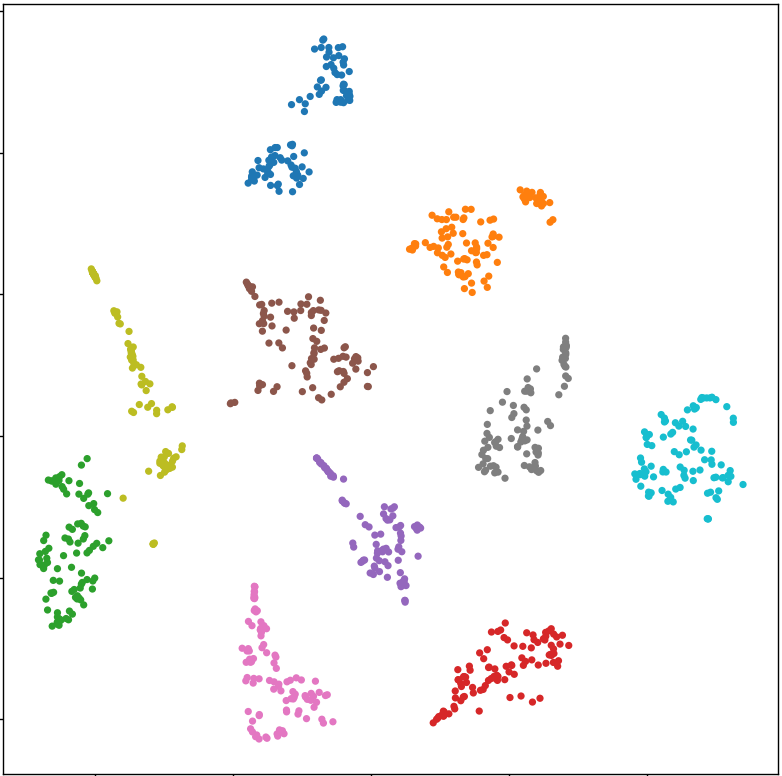
\includegraphics[width=0.25\linewidth]{simsiam_tsne.png}
        \label{simsiam_tsne}
    }
    \subfloat[]{
        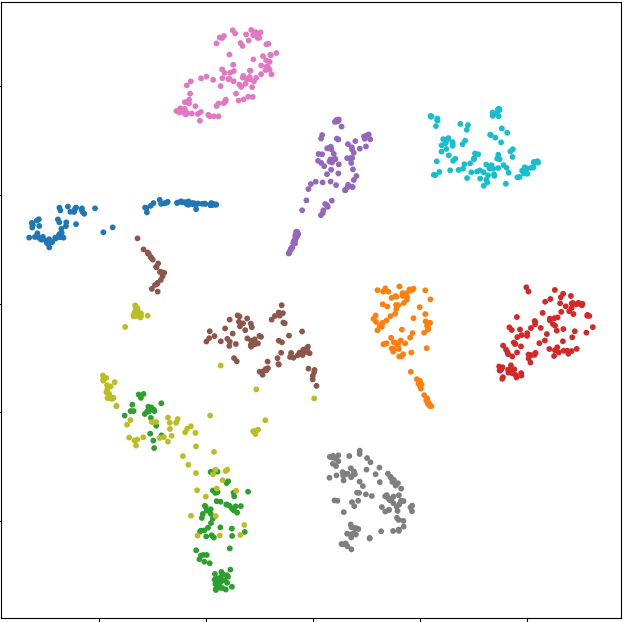
\includegraphics[width=0.25\linewidth]{simclr_batch_size_16.png}
        \label{simclr_tsne}
    }
    \subfloat[]{
        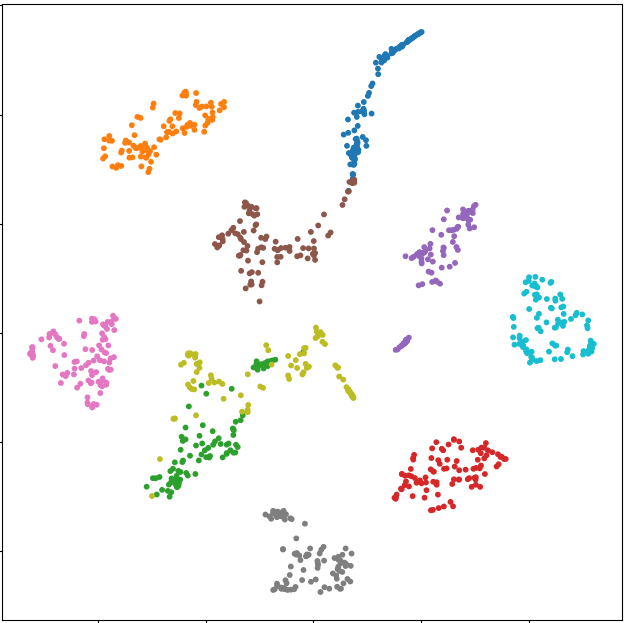
\includegraphics[width=0.25\linewidth]{byol_batch_size_128.png}
        \label{byol_tsne}
    }
    \\
    \subfloat[]{
        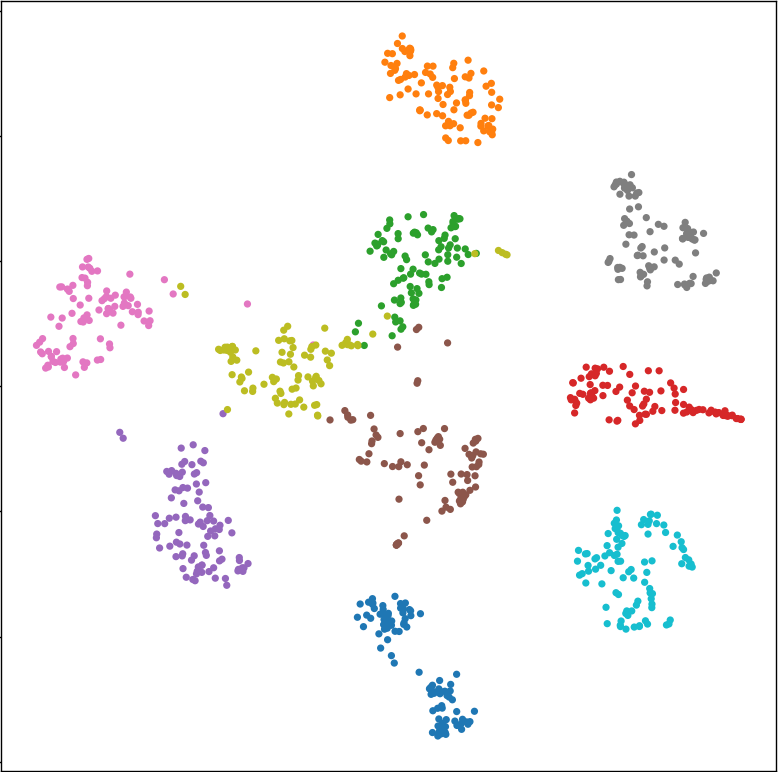
\includegraphics[width=0.25\linewidth]{cnn_tsne.png}
        \label{cnn_tsne}
    }
    \subfloat[]{
        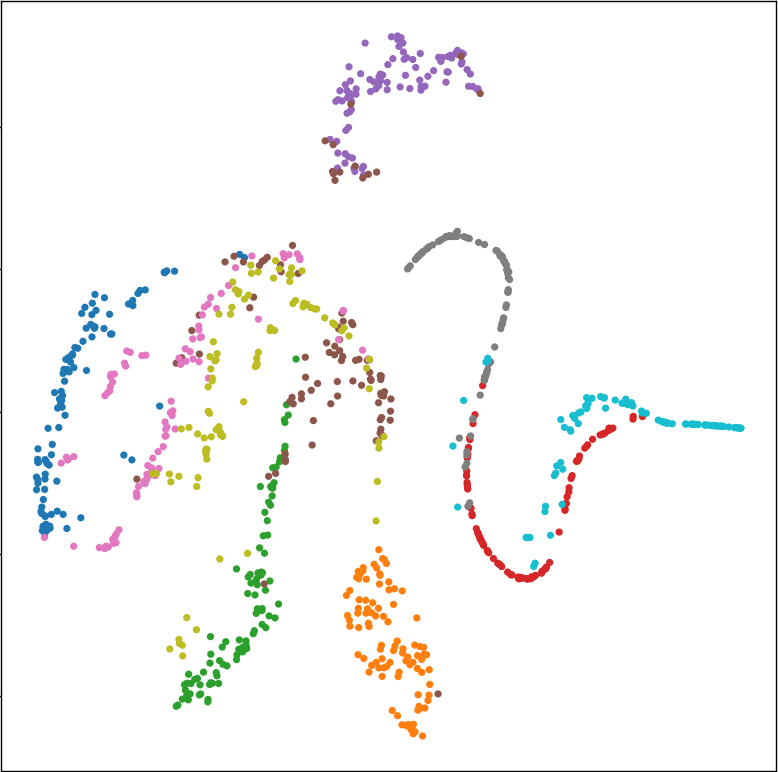
\includegraphics[width=0.25\linewidth]{svm_tsne.png}
        \label{svm_tsne}
    }
    \caption{验证集数据经特征提取的 T-SNE 可视化:(a) SimSiam 的 T-SNE 分布图;(b) SimCLR 的 T-SNE 分布图;(c) BYOL 的 T-SNE 分布图;(d) CNN 的 T-SNE 分布图;(e) SVM 的 T-SNE 分布图}
    \label{tsne_of_all_models}
\end{figure}

\subsection{对SimSiam网络Stop-Grad模块和Predictor模块的探讨}
\label{sec:discuss_of_simsiam_module}

\begin{figure}
    \centering
    \subfloat[]{
        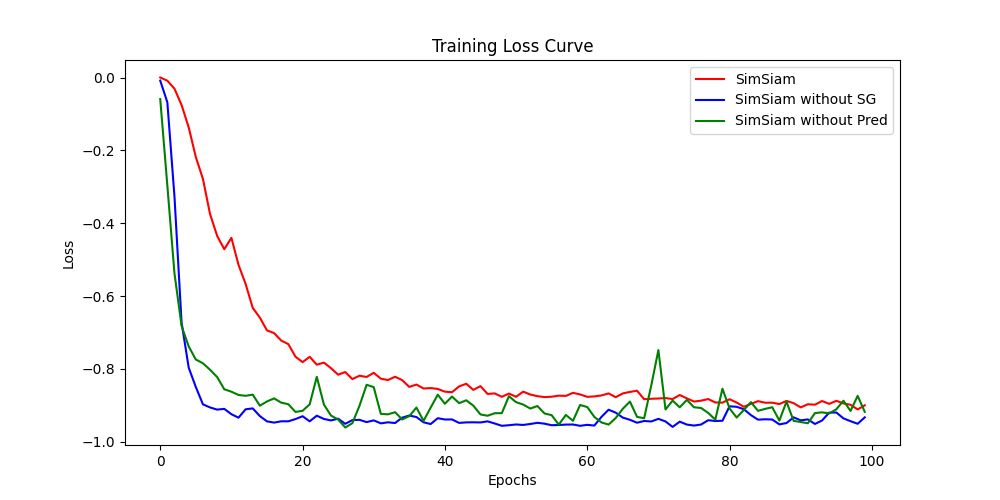
\includegraphics[width=0.45\linewidth]{loss.png}
        \label{train_process_simsiam_discuss:loss}
    }
    \subfloat[]{
        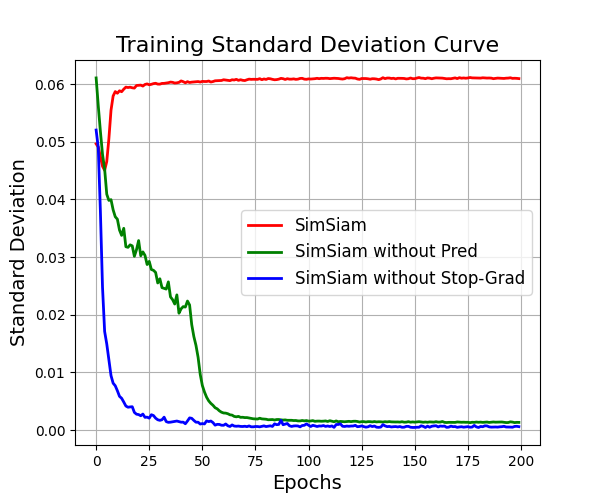
\includegraphics[width=0.45\linewidth]{std.png}
        \label{train_process_simsiam_discuss:std}
    }\\
    \subfloat[]{
        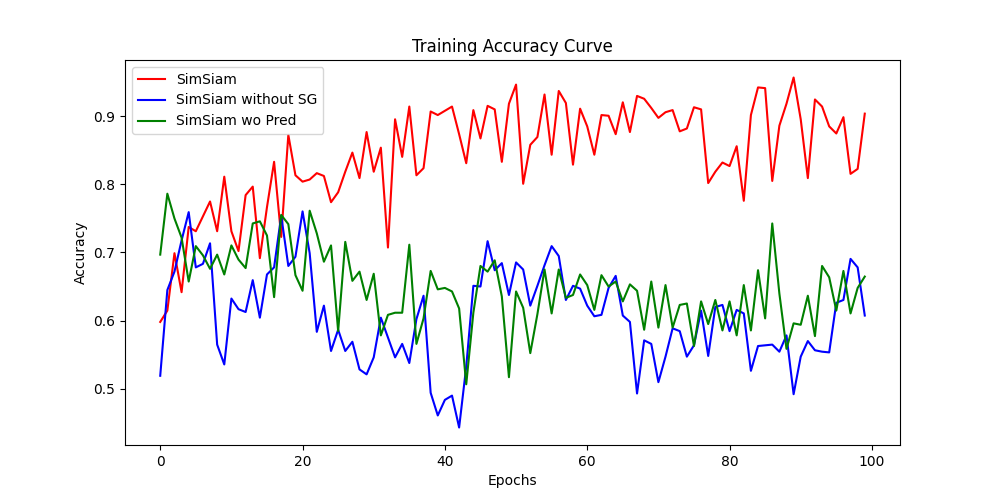
\includegraphics[width=0.45\linewidth]{acc.png}
        \label{train_process_simsiam_discuss:acc}
    }
    \caption{SimSiam,SimSiam(无Stop-Grad模块)与SimSiam(无预测器模块)的训练过程对比(a) 损失函数;(b) 提取特征的标准差;(c) K-Means聚类准确率}
    \label{train_process_simsiam_discuss}
\end{figure}

\begin{figure}
    \centering
    \subfloat[]{
        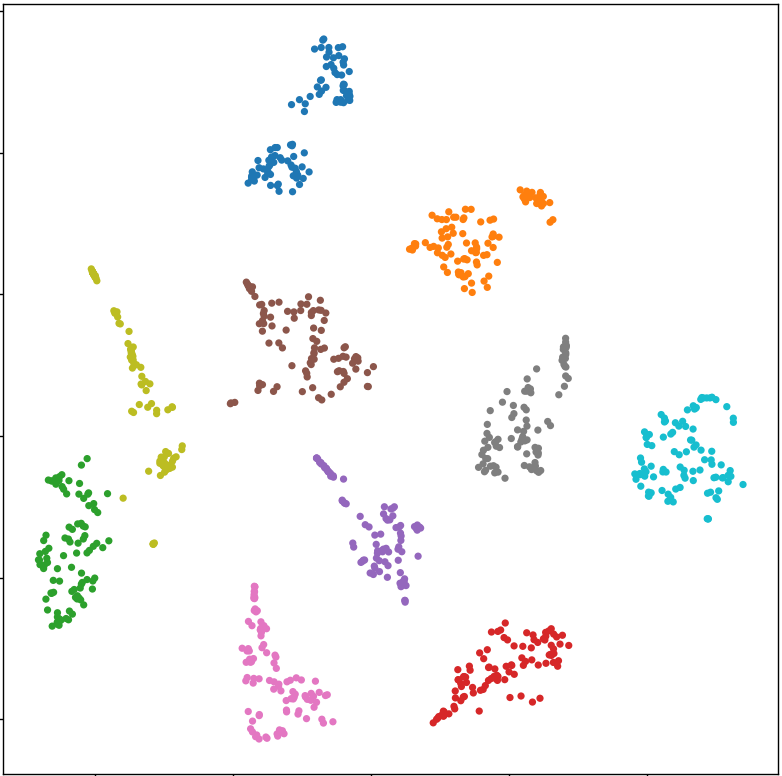
\includegraphics[width=0.3\linewidth]{simsiam_tsne.png}
        \label{tsne_simsiam_discuss:simsiam_tsne}
    }
    \subfloat[]{
        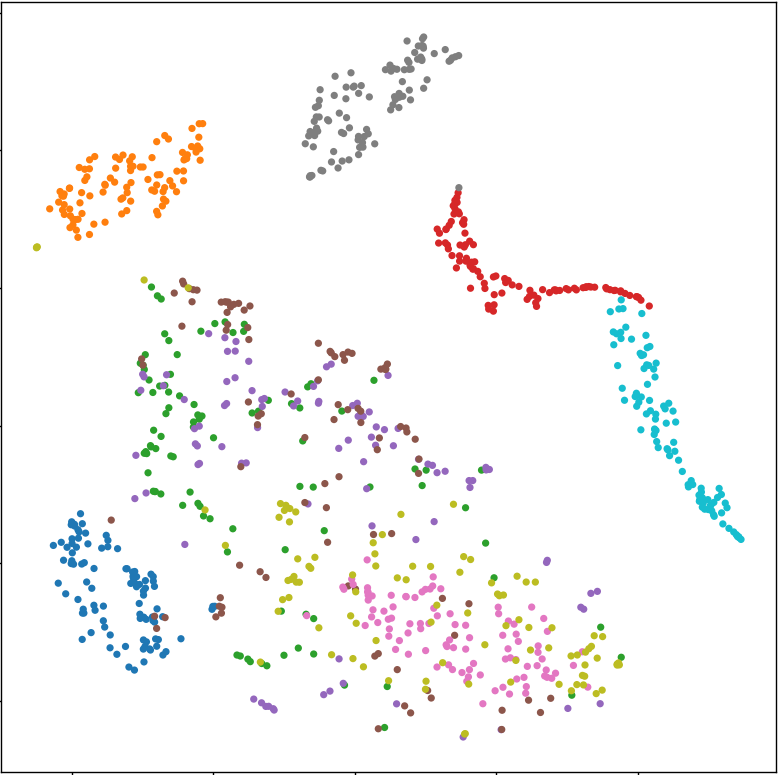
\includegraphics[width=0.3\linewidth]{simsiam_wo_stopgrad_tsne.png}
        \label{tsne_simsiam_discuss:simsiam_wo_stopgrad_tsne}
    }
    \subfloat[]{
        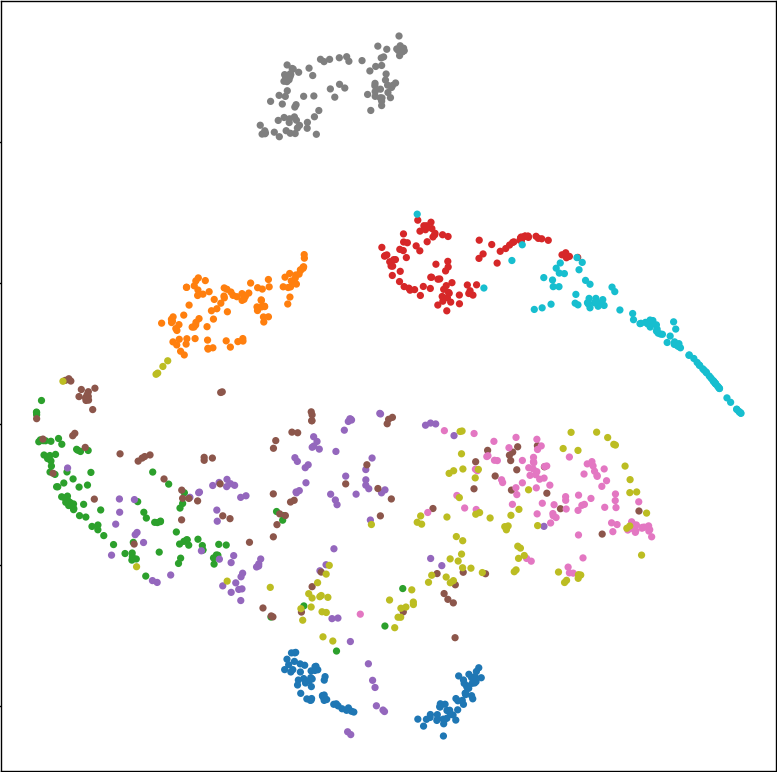
\includegraphics[width=0.3\linewidth]{simsiam_wo_pred_tsne.png}
        \label{tsne_simsiam_discuss:simsiam_wo_pred_tsne}
    }
    \caption{SimSiam,SimSiam(无Stop-Grad模块)与SimSiam(无预测器模块)的T-SNE图(a) SimSiam;(b) SimSiam without Stop-Grad;(c) SimSiam without Predictor}
    \label{tsne_simsiam_discuss}
\end{figure}

\begin{table}
    \caption{SimSiam、SimSiamw/o SG 与 SimSiamw/o Pred 在不同 $\beta$ 值下的准确率}
    \centering
    \begin{tabular}{cccc}
    \toprule
    不平衡因子$\beta$  & SimSiam & SimSiamw/o SG & SimSiamw/o Pred \\
    \midrule
    1   & 0.9515  & 0.5338  & 0.5217 \\
    10  & 0.9402  & 0.4919  & 0.4604 \\
    50  & 0.9131  & 0.3579  & 0.3892 \\
    100 & 0.8450  & 0.3412  & 0.3704 \\
    \midrule
    平均值 & 0.9125 & 0.4312 & 0.4354\\
    \bottomrule
    \end{tabular}
    \label{simsiam_vs_simsiamwosg_wopred}
\end{table}

图\ref{train_process_simsiam_discuss}展示了“使用停止梯度(Stop-Grad)”与“不使用停止梯度”的比较。架构和所有超参数保持不变,唯一的区别是是否使用停止梯度或预测器。
图\ref{train_process_simsiam_discuss:loss}显示了训练损失。不使用停止梯度时,优化器迅速找到一个退化解,并达到最小可能损失 \(-1\)。为了证明这种退化是由坍缩引起的,我们研究了 \(\ell_2\) 归一化输出 \( z / \|z\|_2 \) 的标准差(std)。如果输出坍缩到一个常数向量,则所有样本的 std 在每个通道上应该为零。这可以从图 2(中)的红色曲线中观察到。


作为对比,如果输出 \( z \) 具有零均值各向同性高斯分布,我们可以证明 \( \frac{z}{\|z\|_2} \) 的标准差为 \( \frac{1}{\sqrt{d}} \)。下证:假设 \( z \in \mathbb{R}^d \) 是一个零均值各向同性高斯分布,即 \( z \sim \mathcal{N}(0, I_d) \),其中 \( I_d \) 是 \( d \) 维单位矩阵,表示协方差矩阵为单位矩阵,意味着每个分量 \( z_i \) 独立且服从标准正态分布。我们需要证明的是,\( \frac{z}{\|z\|_2} \) 的标准差(即每个分量的标准差)为 \( \frac{1}{\sqrt{d}} \),其中 \( \|z\|_2 = \sqrt{\sum_{i=1}^{d} z_i^2} \) 是 \( z \) 的 \( L_2 \) 范数。

\textbf{证明步骤}:

\begin{enumerate}
    \item \textbf{标准化操作}:
    设 \( z = (z_1, z_2, \dots, z_d) \),则 \( z \) 的每个分量 \( z_i \) 都是独立的标准正态随机变量 \( z_i \sim \mathcal{N}(0, 1) \),并且 \( \|z\|_2 = \sqrt{\sum_{i=1}^{d} z_i^2} \) 是 \( z \) 的欧几里得范数。我们关注的是向量 \( \frac{z}{\|z\|_2} \) 的每个分量。

    \item \textbf{定义随机变量}:
    令 \( \hat{z} = \frac{z}{\|z\|_2} \),即 \( \hat{z} \) 是单位向量,表示将 \( z \) 投影到单位球面上的结果。

    \item \textbf{每个分量的分布}:
    因为 \( z \) 是各向同性高斯分布,其方向是均匀分布在单位球面上的。对于标准化后的向量 \( \hat{z} \),每个分量 \( \hat{z}_i = \frac{z_i}{\|z\|_2} \) 的分布不再是标准正态分布,而是受到范数约束的结果。

    \item \textbf{期望值和方差}:
    由于 \( z \) 是各向同性的,\( \hat{z}_i \) 的分布是对称的,所有分量 \( \hat{z}_i \) 的期望值为 0。因此,接下来我们计算 \( \hat{z}_i \) 的方差。

    对于 \( \hat{z}_i \) 的方差,我们有:
    \begin{equation}
    \text{Var}(\hat{z}_i) = \mathbb{E}[\hat{z}_i^2] - (\mathbb{E}[\hat{z}_i])^2
    \end{equation}
    由于 \( \mathbb{E}[\hat{z}_i] = 0 \),我们只需要计算 \( \mathbb{E}[\hat{z}_i^2] \)。

    \begin{equation}
    \mathbb{E}[\hat{z}_i^2] = \mathbb{E}\left[\frac{z_i^2}{\|z\|_2^2}\right] = \frac{\mathbb{E}[z_i^2]}{\mathbb{E}[\|z\|_2^2]} = \frac{1}{d}
    \end{equation}
    其中 \( \mathbb{E}[z_i^2] = 1 \)(因为 \( z_i \) 是标准正态分布),而 \( \mathbb{E}[\|z\|_2^2] = \mathbb{E}[\sum_{i=1}^{d} z_i^2] = d \),因为每个 \( z_i^2 \) 的期望为 1。

    \item \textbf{标准差}:
    由于方差 \( \text{Var}(\hat{z}_i) = \frac{1}{d} \),因此标准差是:
    \begin{equation}
    \text{std}(\hat{z}_i) = \frac{1}{\sqrt{d}}
    \end{equation}
\end{enumerate}


图\ref{train_process_simsiam_discuss:std}的红色曲线显示,使用停止梯度时,std 值接近 \( \frac{1}{\sqrt{d}} \)。这表明输出没有坍缩,而是分散在单位超球面上。
图\ref{train_process_simsiam_discuss:acc}绘制了KMeans聚类的验证准确率。KMeans聚类可以作为进展的监控工具。使用停止梯度时,监控显示出准确率稳步提高。

图\ref{train_process_simsiam_discuss}的绿色曲线显示模型在移除预测器(Predictor)后的表现,可以看出移除预测器后发生了与移除Stop-Grad类似的坍塌。事实上,如果使用对称损失(式(\ref{eq:cos_loss})),这一现象是可以预期的。现在的损失函数是
\begin{equation}
    \frac{1}{2}D(z_1, \text{stopgrad}(z_2)) + \frac{1}{2}D(z_2, \text{stopgrad}(z_1)).
\end{equation}
其梯度的方向与 $D(z_1, z_2)$ 的梯度相同,只不过幅度被缩放了 $\frac{1}{2}$。在这种情况下,移除Stop-Grad相当于将损失函数缩放为$\frac{1}{2}$。这一调整导致了模型的崩溃(见图\ref{train_process_simsiam_discuss})。图\ref{tsne_simsiam_discuss}进一步可视化了该崩溃对特征提取的影响:在移除Stop-Grad或预测器后,特征空间中的大量样本交叉重叠,导致其变得难以区分。
表\ref{simsiam_vs_simsiamwosg_wopred}也显示了移除Stop-Grad或预测器后的巨大性能损失。我们的实验表明,Stop-Grad模块对防止模型塌陷起到至关重要的作用,当移除该模块后,通过观察最小可能的损失值以及模型输出的常数性(标准差),可以发现这种塌陷现象。塌陷解的存在表明,仅通过架构设计(如预测器、BN、$\ell_{2}$-范数)来防止塌陷是不充分的。

引入停止梯度的设计暗示了另一个潜在的优化问题正在被隐式解决。SimSiam 是一种类似于期望最大化(EM)算法的实现。它隐式地涉及两组变量,并解决两个潜在的子问题。停止梯度操作的出现是引入额外变量集的后果。

我们考虑以下形式的损失函数:
\begin{equation}
\label{eq:loss}
\mathcal{L}(\theta,\eta)=\mathbb{E}_{x,\mathcal{T}}\left[\|\mathcal{F}_{\theta} (\mathcal{T}(x))-\eta_{x}\|^{2}_{2}\right].
\end{equation}
其中,$\mathcal{F}$ 是由 $\theta$ 参数化的网络,$\mathcal{T}$ 是数据增强,$x$ 是输入样本。期望 $\mathbb{E}[\cdot]$ 是对输入样本和数据增强的分布进行的。为了便于分析,这里我们使用均方误差 $\|\cdot\|^{2}_{2}$,如果向量是 $\ell_{2}$-归一化的,则等效于余弦相似度。我们暂时不考虑预测器,稍后再讨论。

在式(\ref{eq:loss})中,我们引入了另一组变量,记为 $\eta$。$\eta$ 的大小与输入样本数量成正比。直观上,$\eta_{x}$ 是输入样本 $x$ 的表示,下标 ${}_{x}$ 表示使用输入样本索引访问 $\eta$ 的子向量。$\eta$ 不一定是网络的输出;它是一个优化问题的参数。

通过这种形式化,我们考虑解决以下问题:
\begin{equation}
\label{eq:min_loss}
\min_{\theta,\eta}\mathcal{L}(\theta,\eta).
\end{equation}
这里的问题是针对 $\theta$ 和 $\eta$ 的。这种形式化类似于 KMeans 聚类。变量 $\theta$ 类似于聚类中心:它是编码器的可学习参数。变量 $\eta_{x}$ 类似于样本 $x$ 的分配向量(在 KMeans 中是一个 one-hot 向量):它是 $x$ 的表示。

同样类似于 KMeans,式(\ref{eq:min_loss})中的问题可以通过交替算法解决,固定一组变量并解决另一组变量。形式上,我们可以在以下两个子问题之间交替:
\begin{equation}
\label{eq:theta_subproblem}
\theta^{t} \leftarrow \arg\min_{\theta}\;\mathcal{L}(\theta,\eta^{t-1})
\end{equation}
\begin{equation}
\label{eq:eta_subproblem}
\eta^{t} \leftarrow \arg\min_{\eta}\;\mathcal{L}(\theta^{t},\eta)
\end{equation}
其中,$t$ 是交替的索引,“$\leftarrow$”表示赋值。

\textbf{求解 $\theta$}:可以使用随机梯度下降(SGD)来解决子问题(\ref{eq:theta_subproblem})。停止梯度操作是一个自然的结果,因为梯度不会反向传播到 $\eta^{t-1}$,而 $\eta^{t-1}$ 在这个子问题中是一个常数。

\textbf{求解 $\eta$}:子问题 (\ref{eq:eta_subproblem}) 可以独立地为每个 $\eta_{x}$ 求解。现在的问题是最小化:$\mathbb{E}_{\mathcal{T}}\left[\|\mathcal{F}_{\theta^{t}}(\mathcal{T}(x))-\eta_{x} \|_{2}^{2}\right]$,其中期望是对数据增强 $\mathcal{T}$ 的分布进行的。由于使用均方误差,可以通过以下方式轻松求解:

\begin{equation}
\label{eq:eta_update}
\eta_{x}^{t}\leftarrow\mathbb{E}_{\mathcal{T}}\Big{[}\mathcal{F}_{\theta^{t}}( \mathcal{T}(x))\Big{]}.
\end{equation}

这表明 $\eta_{x}$ 被赋值为 $x$ 在数据增强分布上的平均表示。

\textbf{单步交替:} SimSiam 可以通过在式(\ref{eq:theta_subproblem})和式(\ref{eq:eta_subproblem})之间进行一次交替来近似。首先,我们通过仅对数据增强采样一次(记为 $\mathcal{T}^{\prime}$)并忽略 $\mathbb{E}_{\mathcal{T}}[\cdot]$ 来近似式(\ref{eq:eta_update}):

\begin{equation}
\label{eq:eta_approx}
\eta_{x}^{t}\leftarrow\mathcal{F}_{\theta^{t}}(\mathcal{T}^{\prime}(x)).
\end{equation}

将其代入子问题 (\ref{eq:theta_subproblem}),我们得到:

\begin{equation}
\label{eq:theta_update}
\theta^{t+1}\leftarrow\arg\min_{\theta}\mathbb{E}_{x,\mathcal{T}}\Big{[}\big{\| }\mathcal{F}_{\theta}(\mathcal{T}(x))-\mathcal{F}_{\theta^{t}}(\mathcal{T}^{ \prime}(x))\big{\|}_{2}^{2}\Big{]}.
\end{equation}

现在 $\theta^{t}$ 在这个子问题中是一个常数,而 $\mathcal{T}^{\prime}$ 由于其随机性暗示了另一个视图。这种形式化展示了孪生网络架构。其次,如果我们通过一步 SGD 减少损失来实现式(\ref{eq:theta_update}),那么我们可以接近 SimSiam 算法:一个自然带有停止梯度操作的孪生网络。

\textbf{预测器:} 根据定义,预测器 $h$ 期望最小化:
\begin{equation}
\mathbb{E}_{x}\Big{[}\big{\|}h(z_{1})-z_{2}\big{\|}_{2}^{2}\Big{]} 
\label{eq:target_of_h}
\end{equation}
其中,$z_i = \mathcal{F}(x_i)$,$x_i$表示输入$x$的第$i$个视图。$h$ 的最优解应满足:对于任何输入$x$, $h(z_{1})\!=\!\mathbb{E}_{z}[z_{2}]\!=\!\mathbb{E}_{\mathcal{T}}\big{[}\mathcal{F}( \mathcal{T}(x))\big{]}$ 。这个项类似于式(\ref{eq:eta_update})中的项。在式(\ref{eq:eta_approx})的近似中,期望 $\mathbb{E}_{\mathcal{T}}[\cdot]$ 被忽略了。$h$ 的使用可能填补了这一空白。在实践中,实际计算期望 $\mathbb{E}_{\mathcal{T}}$ 是不现实的。但神经网络(例如预测器 $h$)可能能够学习预测期望,而 $\mathcal{T}$ 的采样隐式分布在多个 epoch 中。

\textbf{数据增强:} 根据上述讨论,$h$ 的最优解应满足 $h(z_1) = \mathbb{E}_z[z_2]$。假设 $h$ 为线性映射,则有 $h(\mathbb{E}[z_1]) = \mathbb{E}[z_2]$。同时,根据对称损失函数式(\ref{eq:cos_loss}),$h$ 的最优解应满足 $h(z_2) = \mathbb{E}_z[z_1]$。将此关系代入,得到 $h(\mathbb{E}[z_1]) = \mathbb{E}[z_2]$,进一步推导得 $h(h(z_2)) = \mathbb{E}[z_2]$。因此,式(\ref{eq:derivation_of_h})可表示为:

\begin{equation}
    h(h(x)) = \mathbb{E}[x]
    \label{eq:derivation_of_h}
\end{equation}

这表明,在满足最优解的条件下,$h$ 很可能是输入变量 $x$ 到其期望值的平滑映射。假设 $h = \mathbb{E}$,显然这是式(\ref{eq:derivation_of_h})的一个特解。基于此,子问题(\ref{eq:theta_subproblem})可以表述为:

\begin{equation}
    \arg\min_{\theta} \left[\| \mathcal{F}_{\theta}(x_1) - \mathbb{E}(z_2) \|_2^2 + \| \mathcal{F}_{\theta}(x_2) - \mathbb{E}(z_1) \|_2^2 \right]
\end{equation}

因此,SimSiam 的目标是最小化两个视图 \( x_1 \) 和 \( x_2 \) 输出特征期望值之间的距离,即使得 \( \mathbb{E}(\mathcal{F}_\theta(x_1)) = \mathbb{E}[z_2] \) 且 \( \mathbb{E}(\mathcal{F}_\theta(x_2)) = \mathbb{E}[z_1] \),从而促使模型学习到在数据增强下保持不变的深层次语义。图 \ref{simsiam_derivation_of_features} 直观展示了模型训练前后特征分布的变化。在训练前,多个相似样本的两个视图的特征在特征空间中可能位于距离较远且形态各异的区域;而在训练后,两个视图的特征空间趋于重叠,且期望值之间的距离显著缩小。这表明,编码器成功学习到了对数据增强不敏感的深层次语义特征。此时,当 \( h \) 计算出 \( \mathbb{E}[z_1] \) 时,即可得到式(\ref{eq:target_of_h})的最优解,对于 \( z_2 \) 同理。

然而,如果数据增强模块没有有效地带来多样化的特征空间分布(例如,训练前两个视图的特征空间已经趋于重叠),那么当 \( h \) 学习到期望值时,编码器可能不再需要进一步学习那些与数据增强无关的深层语义特征。

\begin{figure}[h]
    \centering
    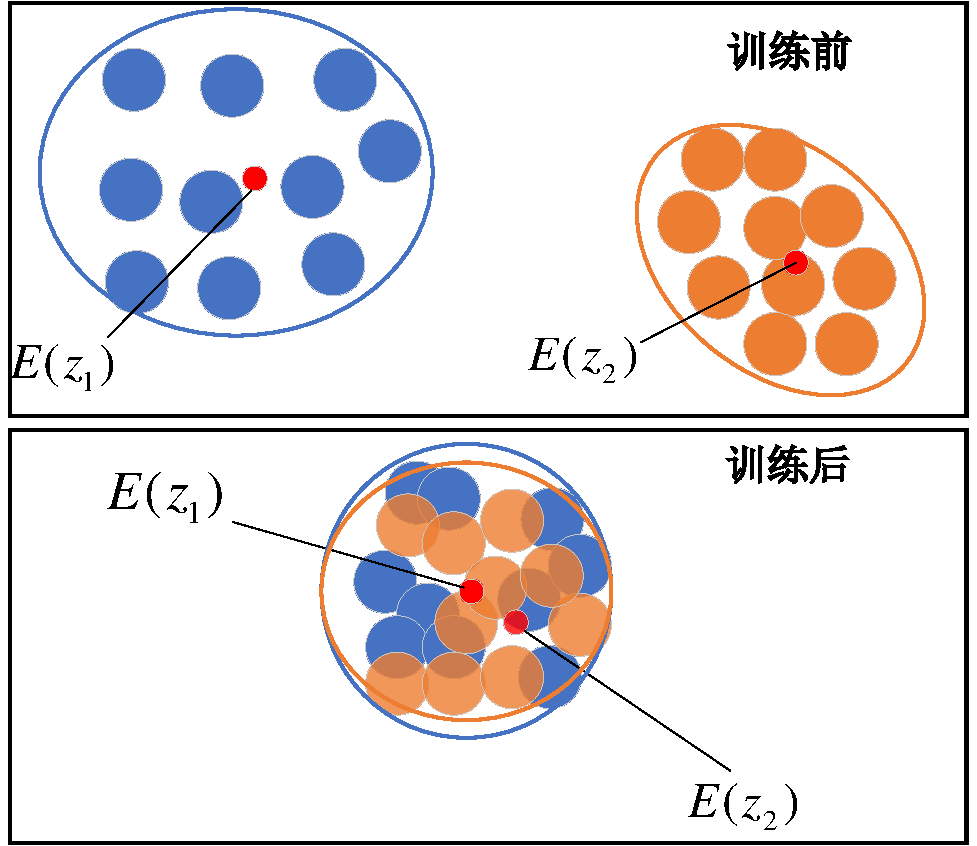
\includegraphics[width=12cm]{simsiam_derivation_of_features.pdf}
    \caption{不同视图的模型特征输出分布的变化示意图}
    \label{simsiam_derivation_of_features}
\end{figure}

\subsection{对数据增强模块的探讨}
在\ref{sec:CMA-ES_result}小节,我们在限定范围内求得了各个数据增强子策略的最优参数解,并在之后的实验中取得了良好的结果。本节讨论表\ref{CMA-ES_solution}中的8个数据增强子策略对模型性能的影响。图\ref{train_process_da_discuss}显示了移除单个子策略后模型训练过程中的损失函数及特征标准差。表\ref{tb:da_discuss_results}移除不同数据增强子策略的准确率性能变化。

在本节中,我们分析了不同数据增强方法对模型性能的影响。具体而言,我们讨论了以下几种增强技术:缩放、块打乱和掩码、高斯噪声和相位扰动、绝对值以及竖直翻转和水平翻转。

首先,缩放操作对模型性能的影响最为显著。从表\ref{tb:da_discuss_results}的结果可以看出,移除缩放数据增强后,模型的性能显著下降。振动信号的幅值在时间轴上并非稳定,而是存在波动,这表明信号的特征在不同的尺度和幅度上有变化。引入缩放操作后,模型能够在较小的时间范围内提取出更大幅值范围的特征,从而增强了模型的泛化能力。缺少缩放操作后,模型在不同幅度范围内的鲁棒性降低,导致性能下降。通过增加数据的多样性,缩放操作帮助模型适应了不同的目标尺度和视野范围,进而提升了模型的表现。

其次,块打乱和掩码操作通过局部区域的扰动提高了模型的鲁棒性和对局部特征的提取能力。具体而言,块打乱操作通过打乱图像或信号的局部区域,迫使模型学习局部特征而非依赖全局信息,从而避免模型对局部区域的过度拟合。而掩码操作通过对部分区域进行遮挡,模拟数据中的缺失或遮挡情况,促使模型从有限的信息中恢复或推断出其余部分。这两种数据增强方法在特定场景下,尤其是在存在局部信息缺失或遮挡的情况下,能够有效提升模型的鲁棒性和泛化能力。

高斯噪声和相位扰动主要通过引入轻微的随机噪声或频域变化来增加数据的扰动。尽管这类增强方法能够增加数据的多样性,但其生成的样本与原始数据差异较小,未能有效扩展模型的学习能力,因此对模型性能的影响较为有限。

绝对值操作通过将信号中的负值转化为正值,从而扩展了模型所接触到的样本空间。尤其是在处理具有周期性或对称特征的信号时,绝对值能够引入更多样化的训练样本。这种方法帮助模型适应不同的变化模式,并有效防止模型过早陷入“塌陷”现象。此外,绝对值操作增强了模型对信号反转的鲁棒性,有助于提升模型的泛化能力,特别是在面对多变输入数据时。

最后,竖直翻转和水平翻转操作在处理周期性信号时效果较为有限。周期性信号通常具有特定的模式或周期性变化,这些翻转操作改变了信号的空间结构,但对信号的本质特征影响较小。因此,这两种操作对模型性能的提升相对较弱,尤其是在周期性信号的情况下。

综上所述,不同的数据增强方法对模型性能的提升作用不同。缩放操作显著增加了数据的多样性,提升了模型的泛化能力,因此对模型性能的提升最为显著。其次,块打乱和掩码操作在局部信息缺失或遮挡的情况下有助于提高模型的鲁棒性。尽管高斯噪声和相位扰动对模型性能的提升作用较小,但它们仍然能够增加数据的多样性。最后,绝对值操作有效防止了模型的“塌陷”现象,增强了模型对信号反转的鲁棒性,而竖直翻转和水平翻转的作用较为有限,特别是在处理周期性信号时。

\begin{table}
    \caption{移除不同数据增强子策略在不同 $\beta$ 值下的准确率}
    \centering
    \begin{tabular}{ccccccccc}
    \toprule
    不平衡因子$\beta$  & DA0 & DA1 & DA2 & DA3 & DA4 & DA5 & DA6 & DA7 \\
    \midrule
    1   & 0.9279  & 0.9127 & 0.9254 & 0.9204 & 0.9106 & 0.9298 & 0.9394 & 0.9338  \\
    10  & 0.9258  & 0.9348 & 0.8944 & 0.9298 & 0.8792 & 0.9358 & 0.9333 & 0.9442  \\
    50  & 0.8563  & 0.8379 & 0.8221 & 0.8467 & 0.7490 & 0.8165 & 0.8573 & 0.8387  \\
    100 & 0.7935  & 0.8169 & 0.7356 & 0.7194 & 0.7119 & 0.7912 & 0.8333 & 0.7869  \\
    \midrule
    平均值 & 0.8759 & 0.8756 & 0.8444 & 0.8541 & 0.8127 & 0.8683 & 0.8908 & 0.8759 \\
    \midrule
    相比Baseline & -0.0366 & -0.0369 & -0.0681 & -0.0584 & -0.0998 & -0.0442 & -0.0217 & -0.0366 \\
    \bottomrule
    \end{tabular}
    \label{tb:da_discuss_results}
\end{table}

\begin{figure}[h]
    \centering
    \subfloat[]{
        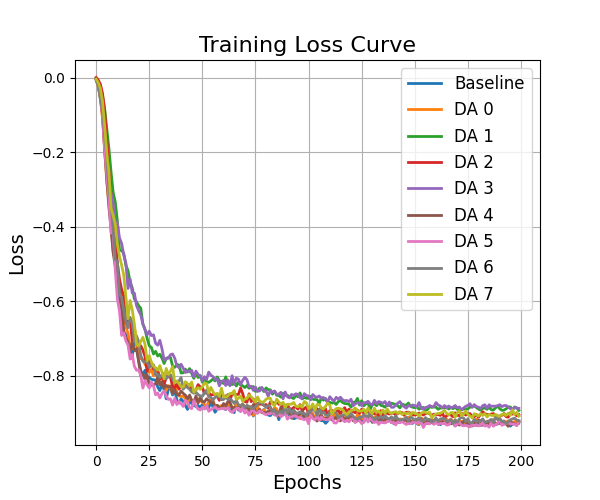
\includegraphics[width=0.45\linewidth]{loss_da.png}
        \label{train_process_da_discuss:loss}
    }
    \subfloat[]{
        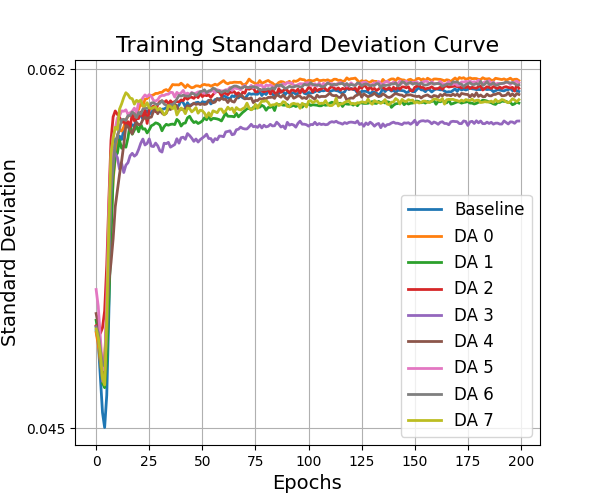
\includegraphics[width=0.45\linewidth]{std_da.png}
        \label{train_process_da_discuss:std}
    }
    \caption{移除不同数据增强子策略的训练过程对比(a) 损失函数;(b) 提取特征的标准差;}
    \label{train_process_da_discuss}
\end{figure}

\subsection{准确率、损失函数和特征标准差之间的相关性分析}

在机器学习和深度学习的模型训练过程中,准确率、损失函数以及特征标准差是评估模型性能和学习过程的重要指标。准确率作为衡量模型预测正确性的标准,通常用于反映模型在分类任务中的表现;而损失函数则用来度量模型输出与真实标签之间的差距,帮助优化算法调整模型参数;特征标准差则能够从一定程度上反映模型“塌陷”的程度,同时反映特征提取的质量。

尽管这些指标分别在不同方面评价模型的表现,但它们之间是否存在内在的相关性,以及这种相关性是否能够提供更深刻的洞察,仍然是值得探讨的问题。准确率与损失函数之间的关系通常较为直观:随着损失函数的减少,模型的预测精度有望提高。然而,特征标准差在此过程中所起的作用可能更加复杂。特征标准差的变化可能在一定程度上影响模型对数据分布的适应能力,进而间接影响最终的准确率。

因此,本节旨在深入探讨准确率、损失函数和特征标准差之间的相关性,通过量化这些指标的关系,揭示它们在模型训练中的互动机制,以便为模型优化和性能提升提供理论依据。通过这一分析,我们可以更全面地理解训练过程中各项指标之间的相互作用,进而指导实际应用中的模型调整与改进。

\textbf{Loss与Std:}表\ref{tb:correlation_with_loss_std}显示了图\ref{train_process_da_discuss}中的Loss曲线与Standard Deviation曲线的皮尔森相关系数(Pearson Correlation)与斯皮尔曼相关系数(Spearman Correlation)。以下是对结果的分析:

在Baseline中,模型包含了所有的数据增强策略,Pearson相关系数为-0.9448,Spearman相关系数为-0.9232。这表明,在包含所有增强策略的情况下,Loss与Standard Deviation之间有较强的负相关性。这个相关性表明,随着训练过程中的损失降低,特征的标准差也相应增大,表明模型的提取特征的能力越来越稳定。

Pearson相关系数和Spearman相关系数在许多情况下呈现出相似的趋势,这表明数据增强策略对Loss和标准差的关系影响较为一致。从结果可以看出,不同的增强策略对Loss与Standard Deviation的相关性产生了不同的影响。总的来说,删除高斯噪声、相位扰动和缩放等增强策略在影响Loss与标准差的关系时,表现出了较强的负相关性,表明这些操作增加了数据的多样性或扰动,使得模型更容易适应各种尺度和噪声变化。而像竖直翻转和水平翻转等操作对Loss与标准差的影响较小,表明这些操作对于周期性信号的处理可能并没有显著改变数据的基本特征。因此,在设计数据增强策略时,应该根据具体任务的特性选择合适的增强方法,以最大程度提升模型的鲁棒性和泛化能力。

同时,表\ref{tb:correlation_with_loss_std}显示,SimSiam在去除Stop-Grad模块(SG)或Predictor模块(Pred)后,表现出较高的正相关性,尤其是斯皮尔曼相关系数几乎接近1,这表明准确率与损失/标准差之间呈现较强的等级相关性。这意味着去除这些模块后,损失和标准差的变化对模型性能的影响呈现出更加明显的等级趋势。具体来说,去除Stop-Grad模块后,模型的性能与损失、标准差之间的关系变得更加显著,尤其在SimSiamw/o SG中,斯皮尔曼相关系数高达0.9935,接近1,说明这种关联非常强。

对于去除Predictor模块的情况,尽管皮尔森相关系数仍然较高(0.9735),但斯皮尔曼相关系数较低(0.7907),这表明去除Predictor模块后,损失和标准差的变化对准确率的影响在等级上的一致性有所减弱。这个变化可能揭示了模型在去除Predictor模块后表现出的一定程度的性能下降,尤其是在捕捉复杂模式时的能力受限。

这个相关性也揭示了模型在去除Stop-Grad模块或Predictor模块后的潜在模型崩塌现象。去除这些模块后,模型的性能变化更加显著,且损失与准确率的关系变得更加直接,暗示着模型在这些模块缺失的情况下,可能缺乏必要的学习能力和稳定性,导致性能严重下降或过拟合。这种分析进一步表明,Stop-Grad模块和Predictor模块在SimSiam模型中的重要性,去除这些模块后可能影响模型的稳定性和泛化能力,进而导致性能的大幅波动和模型崩塌现象。这与前文的实验结论相一致。

\begin{table}
    \centering
    \caption{不同增强子策略的Loss与Standard Deviation的相关系数}
    \begin{tabular}{ccc}
        \hline
        \textbf{删除的增强子策略/模块变化} & \textbf{Pearson Correlation} & \textbf{Spearman Correlation} \\
        \hline
        Baseline & -0.9448 & -0.9232 \\
        高斯噪声 (DA0)  & -0.9619 & -0.8994 \\
        相位扰动 (DA1)  & -0.9169 & -0.9365 \\
        块打乱 (DA2)  & -0.9288 & -0.8851 \\
        掩码 (DA3)  & -0.8962 & -0.8904 \\
        缩放 (DA4)  & -0.9775 & -0.8636 \\
        绝对值 (DA5)  & -0.9412 & -0.9064 \\
        竖直翻转 (DA6)  & -0.9500 & -0.9060 \\
        水平翻转 (DA7)  & -0.8457 & -0.6589 \\
        SimSiam w/o SG & 0.8853 & 0.9935 \\
        SimSiam w/o Pred & 0.9735 & 0.7907 \\
        \hline
    \end{tabular}
    \label{tb:correlation_with_loss_std}
\end{table}

\textbf{准确率与Loss/Std:}表\ref{tab:correlation_with_acc}展示了准确率与损失函数(loss)以及标准差(std)之间的相关性分析。具体分析如下:

首先,准确率与损失函数(loss)的相关性分析表明,无论是使用皮尔森相关系数(-0.0048)还是斯皮尔曼相关系数(-0.1557),两者的相关系数都非常接近零,且对应的 p-value 分别为 0.9910 和 0.7128。这些结果表明,准确率与损失函数之间几乎没有线性或等级上的相关性。因此,尽管损失值反映了模型在训练过程中的误差大小,但它与最终的准确率之间并没有明显的联系。

其次,准确率与标准差(std)之间的相关性也表现出较弱的关系。皮尔森相关系数为 0.1972,斯皮尔曼相关系数为 0.2994,二者均较小,说明准确率与标准差之间的线性或等级相关性较弱。同时,p-value 分别为 0.6398 和 0.4713,这意味着这些相关性并不显著。因此,标准差可能未能有效反映模型预测的波动性与准确率之间的关系。

综合来看,表格中的结果表明,准确率与损失以及标准差之间的相关性非常低,无论是线性还是非线性关系都不显著。这可能意味着,尽管损失和标准差是训练过程中非常重要的指标,但它们并不能直接有效地预测最终模型的准确率。在实际应用中,我们可能需要依赖其他更直接的性能指标来评估模型的表现。

\begin{table}
    \centering
    \caption{准确率与不同指标的相关性分析}
    \begin{tabular}{cccc}
    \toprule
    \textbf{指标} & \textbf{相关系数类型} & \textbf{相关系数} & \textbf{p-value} \\
    \midrule
    准确率与Loss     & 皮尔森相关系数   & -0.0048 & 0.9910 \\
    准确率与Loss     & 斯皮尔曼相关系数 & -0.1557 & 0.7128 \\
    准确率与标准差      & 皮尔森相关系数   & 0.1972 & 0.6398 \\
    准确率与标准差      & 斯皮尔曼相关系数 & 0.2994 & 0.4713 \\
    \bottomrule
    \end{tabular}
    \label{tab:correlation_with_acc}
    \end{table}

\begin{figure}[h]
    \centering
    \subfloat[]{
        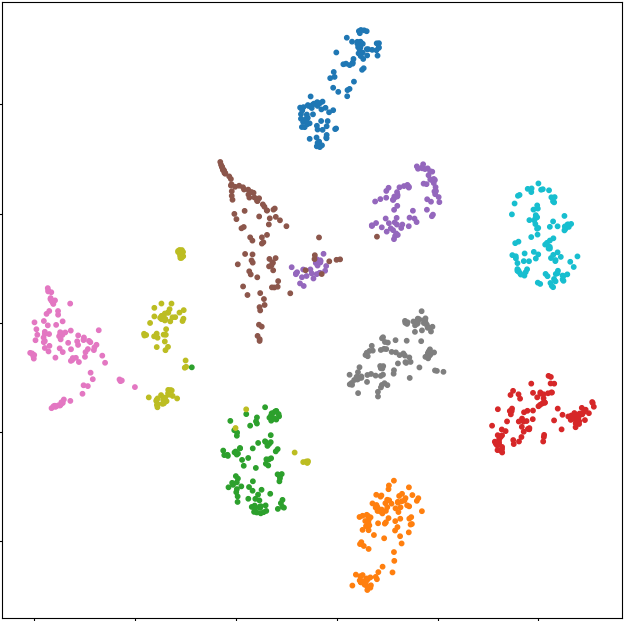
\includegraphics[width=0.3\linewidth]{tsne_ssv_size_10.png}
    }
    \subfloat[]{
        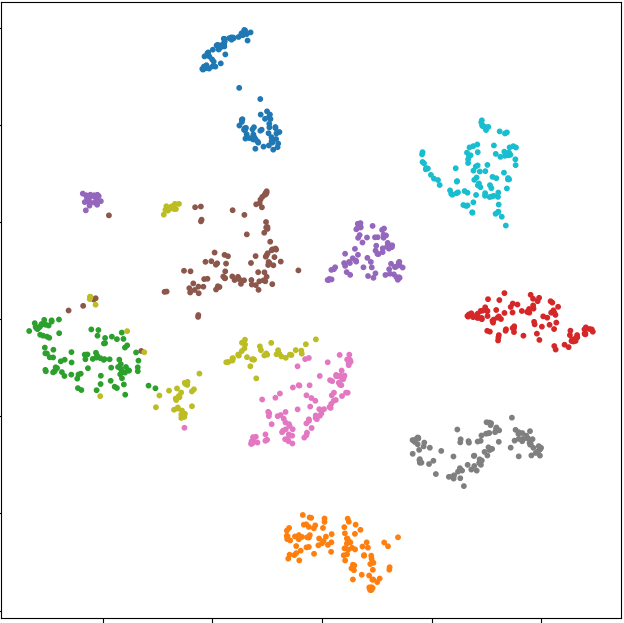
\includegraphics[width=0.3\linewidth]{tsne_ssv_size_20.png}
    }
    \subfloat[]{
        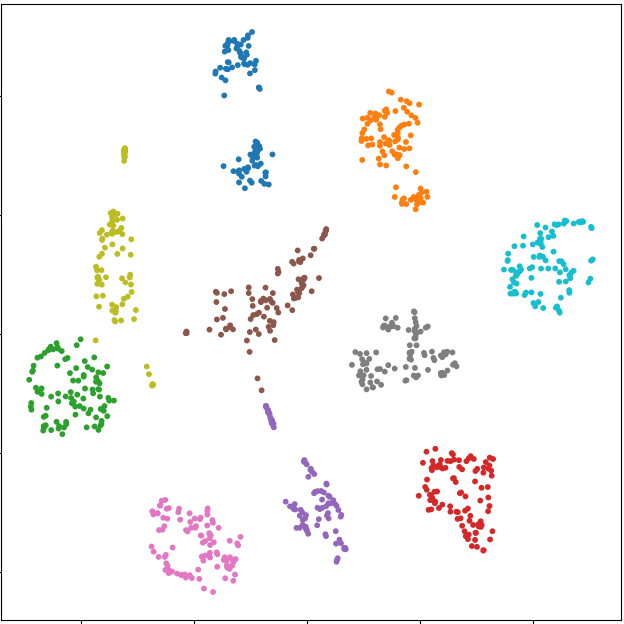
\includegraphics[width=0.3\linewidth]{tsne_ssv_size_50.png}
    }
    \\
    \subfloat[]{
        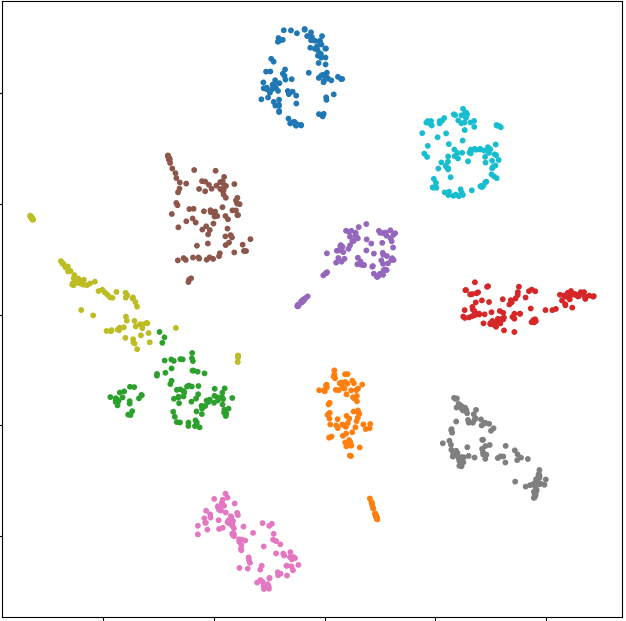
\includegraphics[width=0.3\linewidth]{tsne_ssv_size_100.png}
    }
    \subfloat[]{
        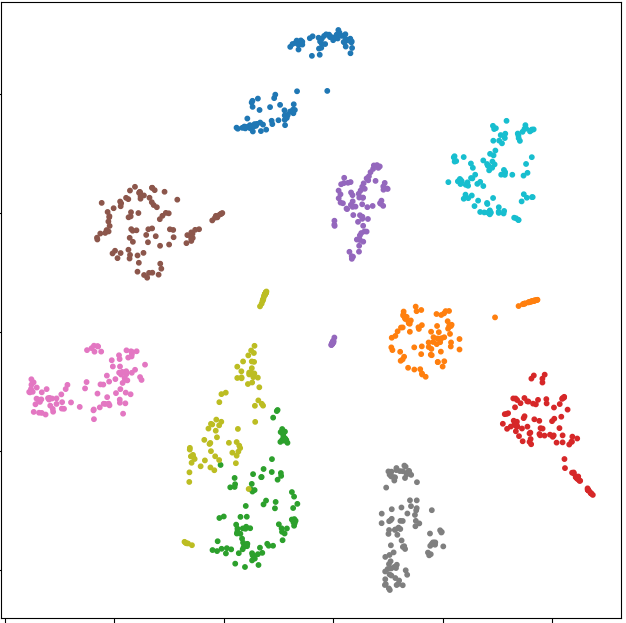
\includegraphics[width=0.3\linewidth]{tsne_ssv_size_150.png}
    }
    \subfloat[]{
        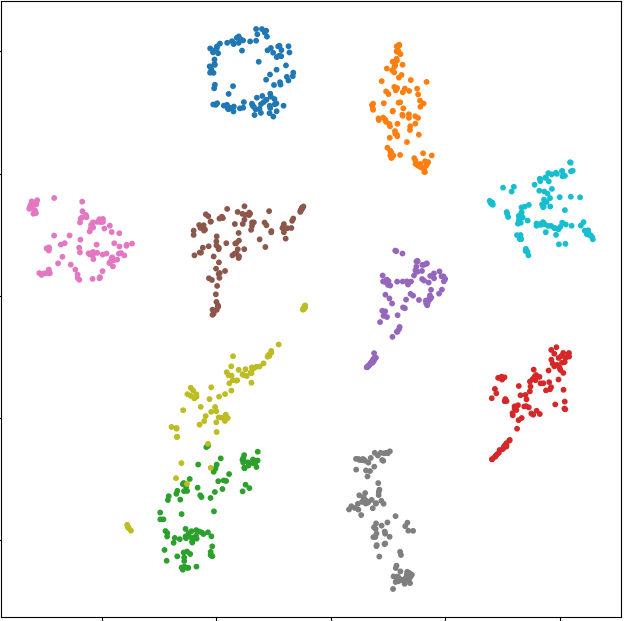
\includegraphics[width=0.3\linewidth]{tsne_ssv_size_200.png}
    }
    
    \caption{不同无标签数据规模的SimSiam网络输出特征的T-SNE分布图:(a) 数据规模为100;(b) 数据规模为200;(c) 数据规模为500;(d) 数据规模为1000;(e) 数据规模为1500;(f) 数据规模为2000}
    \label{tsne_diff_ssv_size}
\end{figure}
\subsection{无标签数据集规模对SimSiam网络性能的影响}
根据前文的讨论,SimSiam网络的性能可能在很大程度上依赖于编码器(Encoder)在无标签数据上进行自监督预训练的质量。本小节旨在探讨无标签样本规模对SimSiam网络性能的影响。实验中,我们固定了训练集的样本规模为100,并分别设置了无标签数据集的规模为100、200、500、1000和2000。通过对比分析,我们评估了不同无标签数据集规模下模型的性能表现。从表\ref{tab:fine_tune_acc_ssv_size}中可以看出,随着无标签数据集规模的增大,模型的性能普遍有所提升,尤其是在较大的数据集规模下,准确率的提升更为显著。

在无标签数据集规模为100时,SimSiam网络的准确率相对较低,尤其是在较大$\beta$值配置下(例如,$\beta=100$时,准确率仅为0.7200)。这一现象表明,在较小的数据集规模下,模型的自监督预训练效果不佳,未能有效地学习到足够的特征,从而导致性能较差。

随着无标签数据集规模的增大,模型的准确率逐渐提升,尤其在数据集规模达到2000时,网络的表现达到最佳,准确率为0.9238。这表明,增加无标签数据集的规模对于模型性能的提升有显著作用。表格中的平均值进一步验证了这一点,随着数据集规模的增加,SimSiam网络的整体表现也逐步提高。在数据集规模为2000时,所有不平衡因子下的平均准确率均较高,凸显了大规模无标签数据集在自监督学习中的重要性。

然而,值得注意的是,当数据规模达到500及以上时,模型性能的提升趋于平稳。通过t-SNE分布图(图\ref{tsne_diff_ssv_size}),可以观察到特征提取质量的改善相对有限,特别是在数据规模从200增加到500时,性能提升最为显著,而从500到2000的提升则较为缓慢。这进一步表明,虽然大规模无标签数据集对模型性能有积极作用,但在一定规模后,性能提升的边际效益逐渐递减。

\begin{table}[h]
    \centering
    \caption{不同无标签数据集规模配置下的SimSiam准确率}
    \begin{tabular}{cccccc}
    \toprule
    无标签数据集规模 & $\boldsymbol{\beta=1}$ & $\boldsymbol{\beta=10}$ & $\boldsymbol{\beta=50}$ & $\boldsymbol{\beta=100}$ & \textbf{平均值} \\
    \midrule
    100   & 0.8988 & 0.8942 & 0.8088 & 0.7200 & 0.8305 \\
    200   & 0.8710 & 0.8642 & 0.7479 & 0.7454 & 0.8071 \\
    500   & 0.9463 & 0.9577 & 0.8713 & 0.7929 & 0.8921 \\
    1000  & 0.9513 & 0.9508 & 0.9025 & 0.8746 & 0.9198 \\
    2000  & 0.9548 & 0.9538 & 0.8946 & 0.8919 & 0.9238 \\
    \bottomrule
    \end{tabular}
    \label{tab:fine_tune_acc_ssv_size}
\end{table}



\subsection{Batch Size对SimSiam网络性能的影响}

\begin{figure}[h]
    \centering
    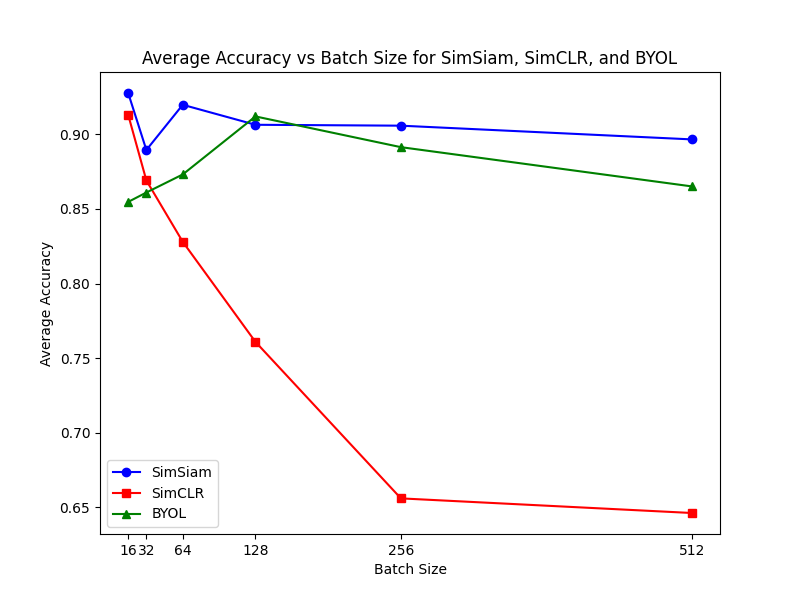
\includegraphics[width=12cm]{acc_of_batch_size.png}
    \caption{不同Batch Size下SimSiam,SimCLR,BYOL的准确率变化图}
    \label{acc_of_batch_size}
\end{figure}

文献\cite{chen2020simple}提到,较大的Batch Size能够显著提高对比学习模型的性能。在本节中,通过实验探讨了不同Batch Size配置下SimSiam网络的表现。表\ref{tab:batch_size_simsiam}展示了不同Batch Size(16, 32, 64, 128, 256, 512)下,SimSiam网络在不同不平衡因子下的准确率。

对于$\beta=1$和$\beta=10$的情况,SimSiam网络在不同Batch Size下的表现相对稳定,唯一的显著性能下降发生在Batch Size为512且$\beta=1$时。这表明,较大的Batch Size可能对模型的训练稳定性产生负面影响,尤其是在低不平衡因子的配置下,可能导致训练过程中出现不稳定现象。

另一方面,针对$\beta=50$和$\beta=100$的配置,当Batch Size较小(16和32)时,模型的准确率表现出较大的波动。这种波动可能与小Batch Size导致的训练不充分或梯度估计不稳定有关。然而,当Batch Size增大至64及以上时,模型表现趋于稳定,说明较大的Batch Size有助于减小训练过程中波动,特别是在高不平衡因子的情况下。

从t-SNE分布图(图\ref{tsne_simsiam_diff_batch_size})中也可以观察到,当Batch Size≥64时,特征提取的质量保持稳定,各个类别的边界更加清晰;而在Batch Size为16或32时,部分点的分布呈现出交叠现象,表明个别点特征分离度较差。综合来看,SimSiam网络的性能对Batch Size的依赖相对较小,整体表现较为稳定,这进一步证明了在一定范围内,Batch Size的增大能够优化训练过程并稳定模型的性能。

反观 \textbf{SimCLR} 在不同 Batch Size 下的表现(见图 \ref{acc_of_batch_size}),随着 Batch Size 的增大,SimCLR模型的准确率呈现出明显的下降趋势,而SimSiam和BYOL的表现稳定,BYOL的性能在Batch Size为128时达到峰值,且是所有不平衡因子下都为最高性能(见表\ref{tab:batch_size_byol_finetune})。从表\ref{tab:batch_size_simclr_finetune}也可以看到,当Batch Size增大,SimCLR在不同不平衡因子的准确率全线下降。表明较大的 Batch Size 可能导致SimCLR模型学习到的特征质量下降。

此外,通过观察 t-SNE 分布图(见图 \ref{tsne_simclr_diff_batch_size}),我们进一步验证了这一现象。在较小的 Batch Size 下,特征的分布较为紧凑,且样本间的区分度较高。然而,随着 Batch Size 的增大,特征分布逐渐变得难以区分,特征提取的质量显著下降。我们推测,这一变化可能与较大 Batch Size 与样本类别总数之比有关。在 SimCLR 中,同一批次中的样本通常被视为负样本,而当 Batch Size 增大时,同一批次中同类别样本的比例更高,从而导致模型倾向于增大同类样本之间的距离,这与对比学习的目标相悖——即相似样本应该聚集。此现象挑战了文献 \cite{chen2020simple} 中提出的“较大的 Batch Size 对对比学习模型性能有益”的观点,表明过大的 Batch Size 可能会损害对比学习的训练效果。

\begin{table}[h]
    \centering
    \caption{不同Batch Size配置下的SimSiam准确率}
    \begin{tabular}{cccccc}
    \hline
    \textbf{Batch Size} & \textbf{$\beta = 1$} & \textbf{$\beta = 10$} & \textbf{$\beta = 50$} & \textbf{$\beta = 100$} & \textbf{平均值} \\
    \hline
    16   & 0.9554 & 0.9567 & 0.9188 & 0.8798 & 0.9277 \\
    32   & 0.9492 & 0.9519 & 0.8600 & 0.7967 & 0.8895 \\
    64   & 0.9513 & 0.9508 & 0.9025 & 0.8746 & 0.9198 \\
    128  & 0.9433 & 0.9498 & 0.8804 & 0.8521 & 0.9064 \\
    256  & 0.9508 & 0.9692 & 0.8900 & 0.8131 & 0.9058 \\
    512  & 0.9258 & 0.9421 & 0.8748 & 0.8435 & 0.8966 \\
    \hline
    \end{tabular}
    \label{tab:batch_size_simsiam}
\end{table}

\begin{table}[h]
    \centering
    \caption{不同Batch Size配置下的SimCLR准确率}
    \begin{tabular}{cccccc}
    \hline
    \textbf{Batch Size} & \textbf{$\beta = 1$} & \textbf{$\beta = 10$} & \textbf{$\beta = 50$} & \textbf{$\beta = 100$} & \textbf{平均值} \\
    \hline
    16   & 0.9208 & 0.9423 & 0.9133 & 0.8760 & 0.9131 \\
    32   & 0.9108 & 0.9090 & 0.8556 & 0.8010 & 0.8691 \\
    64   & 0.8402 & 0.8535 & 0.8323 & 0.7860 & 0.8280 \\
    128  & 0.7935 & 0.8038 & 0.7388 & 0.7073 & 0.7609 \\
    256  & 0.7100 & 0.7292 & 0.6229 & 0.5617 & 0.6560 \\
    512  & 0.7185 & 0.7275 & 0.5940 & 0.5448 & 0.6462 \\
    \hline
    \end{tabular}
    \label{tab:batch_size_simclr_finetune}
\end{table}

\begin{table}[h]
    \centering
    \caption{不同Batch Size配置下的BYOL微调准确率}
    \begin{tabular}{cccccc}
    \hline
    \textbf{Batch Size} & \textbf{$\beta = 1$} & \textbf{$\beta = 10$} & \textbf{$\beta = 50$} & \textbf{$\beta = 100$} & \textbf{平均值} \\
    \hline
    16   & 0.8977 & 0.8977 & 0.8354 & 0.7881 & 0.8547 \\
    32   & 0.8904 & 0.8942 & 0.8481 & 0.8112 & 0.8610 \\
    64   & 0.9200 & 0.9050 & 0.8646 & 0.8029 & 0.8731 \\
    128  & 0.9392 & 0.9529 & 0.8846 & 0.8712 & 0.9120 \\
    256  & 0.9248 & 0.9246 & 0.8517 & 0.8644 & 0.8914 \\
    500  & 0.9267 & 0.9213 & 0.8179 & 0.7946 & 0.8651 \\
    \hline
    \end{tabular}
    \label{tab:batch_size_byol_finetune}
\end{table}

\section{本章小结}
本章节提出了一种结合孪生网络(SimSiam)与基于 CMA-ES 优化器搜索最优数据增强策略的对比学习自监督预训练模型架构,并在构建的服从帕累托长尾分布的 CWRU 数据集上取得了显著的性能提升。通过实验,我们系统地分析了模型架构中各模块的作用,发现 SG(Stop-Grad)模块在模型稳定性方面起到了关键性作用。进一步的实验通过观察模型输出特征的标准差,验证了去除 Stop-Grad 模块或 Predictor 模块后可能导致的潜在崩塌现象,并从理论上揭示了 Predictor 模块与 SG 模块之间的内在联系。

此外,我们详细分析了不同数据增强子模块对模型性能的具体影响。通过进一步研究准确率、损失函数与特征标准差之间的关系,发现损失函数与特征标准差之间呈现预期的负相关性,而当两者相关性为正时,模型可能出现崩塌现象。同时,实验结果表明,准确率与损失函数及特征标准差之间的相关性较低。

最后,通过对不同规模无标签数据集的实验,发现大规模无标签数据集对自监督预训练模型的性能有积极作用,但在达到一定规模后,无标签数据集的规模对性能提升的边际效益逐渐递减。通过对比不同 Batch Size 的实验,发现 SimSiam 网络在不同 Batch Size 下表现出较好的性能稳定性。相比之下,SimCLR 网络在 Batch Size 增大时性能显著下降,表明过大的 Batch Size 可能损害对比学习的训练效果。该实验结果也挑战了文献 \cite{chen2020simple} 中提出的“较大 Batch Size 有益于对比学习模型性能”的观点。

然而,在研究中我们发现,模型微调阶段仍受到由样本分布不平衡引起的偏差影响。为此,在下一章中,我们提出了一种结合半监督学习与 MARC 决策边界调整算法的微调方法,以有效缓解这一问题。

\begin{figure}
    \centering
    \subfloat[]{
        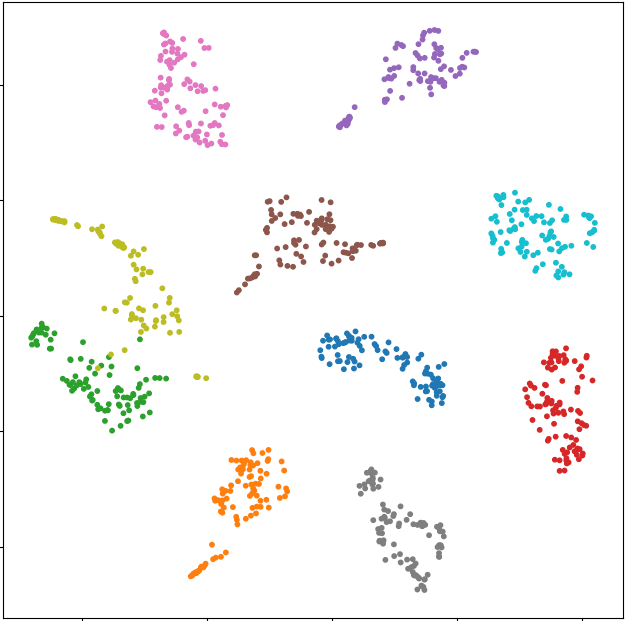
\includegraphics[width=0.25\linewidth]{simsiam_batch_size_16.png}
    }
    \subfloat[]{
        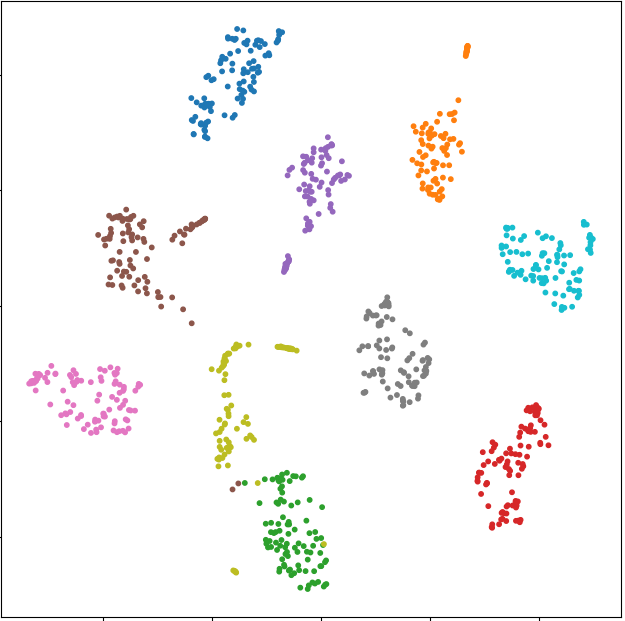
\includegraphics[width=0.25\linewidth]{simsiam_batch_size_32.png}
    }
    \subfloat[]{
        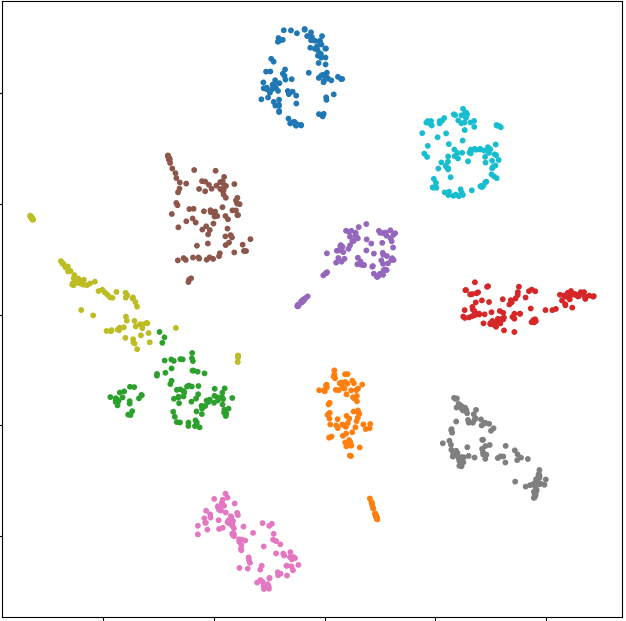
\includegraphics[width=0.25\linewidth]{simsiam_batch_size_64.png}
    }
    \\
    \subfloat[]{
        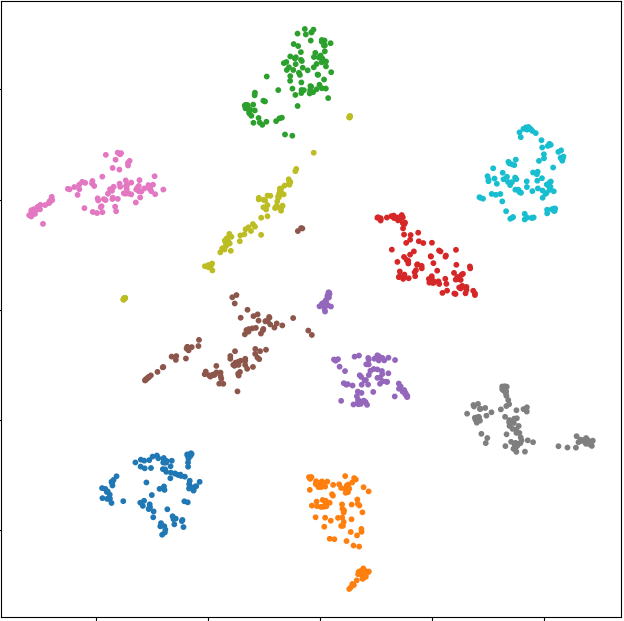
\includegraphics[width=0.25\linewidth]{simsiam_batch_size_128.png}
    }
    \subfloat[]{
        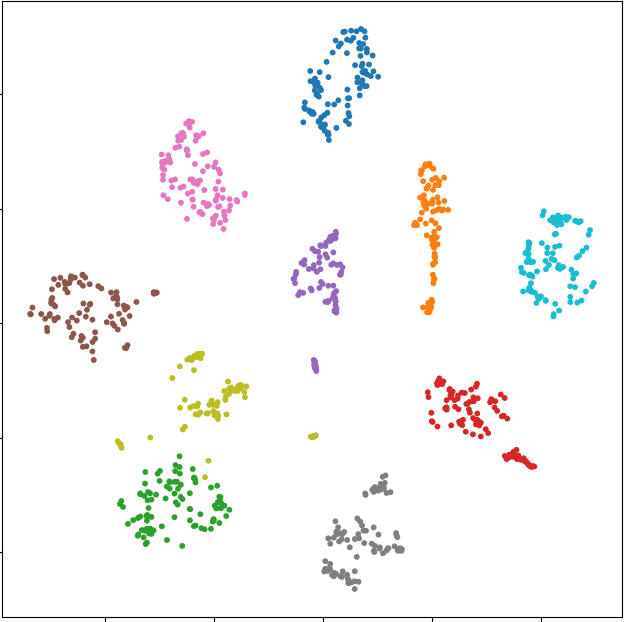
\includegraphics[width=0.25\linewidth]{simsiam_batch_size_256.png}
    }
    \subfloat[]{
        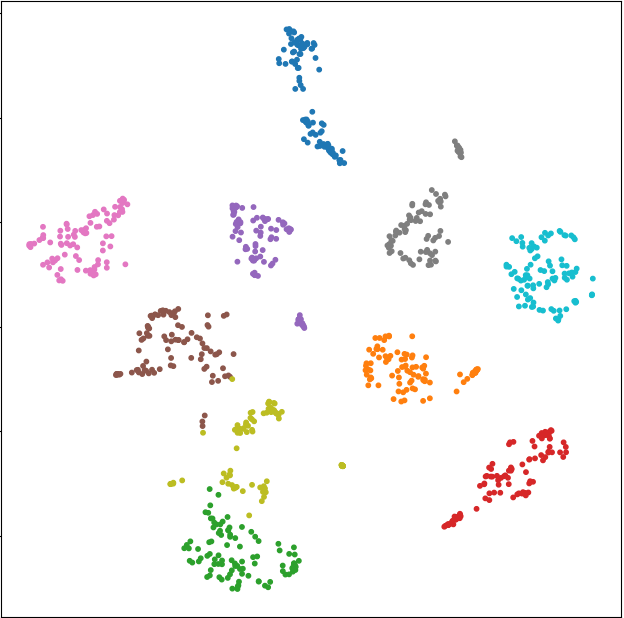
\includegraphics[width=0.25\linewidth]{simsiam_batch_size_512.png}
    }
    
    \caption{不同Batch Size配置下的SimSiam网络输出特征的T-SNE分布图:(a) Batch Size为16;(b) Batch Size为32;(c) Batch Size为64;(d) Batch Size为128;(e) Batch Size为256;(f) Batch Size为512}
    \label{tsne_simsiam_diff_batch_size}
\end{figure}

\begin{figure}
    \centering
    \subfloat[]{
        \includegraphics[width=0.25\linewidth]{simclr_batch_size_16.png}
    }
    \subfloat[]{
        \includegraphics[width=0.25\linewidth]{simclr_batch_size_32.png}
    }
    \subfloat[]{
        \includegraphics[width=0.25\linewidth]{simclr_batch_size_64.png}
    }
    \\
    \subfloat[]{
        \includegraphics[width=0.25\linewidth]{simclr_batch_size_128.png}
    }
    \subfloat[]{
        \includegraphics[width=0.25\linewidth]{simclr_batch_size_256.png}
    }
    \subfloat[]{
        \includegraphics[width=0.25\linewidth]{simclr_batch_size_512.png}
    }
    
    \caption{不同Batch Size配置下的SimCLR网络输出特征的T-SNE分布图:(a) Batch Size为16;(b) Batch Size为32;(c) Batch Size为64;(d) Batch Size为128;(e) Batch Size为256;(f) Batch Size为512}
    \label{tsne_simclr_diff_batch_size}
\end{figure}

\begin{figure}
    \centering
    \subfloat[]{
        \includegraphics[width=0.25\linewidth]{byol_batch_size_16.png}
    }
    \subfloat[]{
        \includegraphics[width=0.25\linewidth]{byol_batch_size_32.png}
    }
    \subfloat[]{
        \includegraphics[width=0.25\linewidth]{byol_batch_size_64.png}
    }
    \\
    \subfloat[]{
        \includegraphics[width=0.25\linewidth]{byol_batch_size_128.png}
    }
    \subfloat[]{
        \includegraphics[width=0.25\linewidth]{byol_batch_size_256.png}
    }
    \subfloat[]{
        \includegraphics[width=0.25\linewidth]{byol_batch_size_512.png}
    }
    
    \caption{不同Batch Size配置下的BYOL网络输出特征的T-SNE分布图:(a) Batch Size为16;(b) Batch Size为32;(c) Batch Size为64;(d) Batch Size为128;(e) Batch Size为256;(f) Batch Size为512}
    \label{tsne_byol_diff_batch_size}
\end{figure}

\chapter{半监督学习和MARC决策面调整相结合的微调方法研究}
在上一章中,我们展示了自监督学习范式下的二阶段式训练方法(如图\ref{self_supervise_procedure}所示),其在故障诊断任务的长尾学习场景中显著提升了模型性能。然而,在微调阶段,样本分布的不平衡问题仍对模型的性能产生不利影响,导致分类器的决策边界发生偏移。如图\ref{decision_edge_bias}所示,决策边界向尾部类特征空间发生偏移,使头部类在特征空间中占据更大的体积,从而降低了尾部类的分类准确率。本章节将重点探讨一种结合半监督学习与MARC决策边界调整的微调算法,以缓解长尾分布对微调阶段决策边界偏移的影响,并进一步提升尾部类的识别能力。

\begin{figure}[h]
    \centering
    \includegraphics[width=12cm]{decision_edge_bias.pdf}
    \caption{由长尾分布带来的决策面偏移示意图}
    \label{decision_edge_bias}
\end{figure}

\section{模型架构}
\subsection{半监督学习模型架构}
本研究提出了一种结合半监督学习与决策边界调整的框架,以有效解决长尾分布和样本不平衡问题。受到文献\cite{yang2020rethinking,wang2023margin}的启发,研究借鉴了半监督学习的经典流程(如图\ref{semi_supervise_procedure}所示)。该流程分为两个阶段:

在第一阶段,使用原始的不平衡标记数据集 $\mathcal{D}_{L}$ 训练一个初步分类器 $f_{\hat{\theta}}$。随后,在第二阶段,利用该分类器对未标记数据集 $\mathcal{D}_{U}$ 进行推断并生成伪标签 $\hat{y}$。伪标签数据与标记数据结合,通过最小化以下损失函数优化模型:
\begin{equation} 
    \mathcal{L}(\mathcal{D}_{L},\theta) + \omega \mathcal{L}(\mathcal{D}_{U},\theta), 
\end{equation}
其中,$\omega$ 为未标记数据的损失权重,$\mathcal{L}(\mathcal{D}_{L},\theta)$ 和 $\mathcal{L}(\mathcal{D}_{U},\theta)$ 分别代表基于标记数据和伪标签数据的损失项。通过整合这两部分损失,最终得到优化后的分类器 $f_{\hat{\theta_f}}$,以更好地建模数据分布,尤其是尾部类别(少数类别)。该过程通过充分利用未标记数据 $\mathcal{D}_{U}$,提升模型对少数类别的分类能力,从而显著优化其决策边界。

\begin{figure}[h]
    \centering
    \includegraphics[width=12cm]{semi_supervise_procedure.pdf}
    \caption{半监督学习流程图}
    \label{semi_supervise_procedure}
\end{figure}

\subsection{MARC决策面调整算法架构}
与此同时,在处理长尾分布和样本不平衡问题时,决策面调整方法(MARC)提供了一种有效的方式来改善分类器的性能,特别是在少数类别(尾部类别)上。文献\cite{wang2023margin}介绍的决策面调整算法通过引入边距校准方法,调整分类器的决策面,使其更加均衡地处理各个类别的数据。

我们发现长尾学习中的边距(Margin)和 logits 存在偏差。边距在图\ref{marc_illustration}中进行了说明。我们定义类别 $ j $ 的仿射超平面 $ H_j \in \mathbb{R}^{p-1} $ 为 $ W_j z + b_j = 0 $,即任何落在超平面 $ H_j $ 正侧的表示点可以归类为类别 $ j $。假设 $ z_0 $ 是一个满足 $ W_j z_0 + b_j = 0 $ 的点,即 $ z_0 $ 在超平面 $ H_j $ 上。假设 $ z_1 $ 是特征空间中的任意点。我们构造从 $ z_0 $ 指向 $ z_1 $ 的向量 $ z_1 - z_0 $,并将其投影到法向量 $ W_j $ 上。投影向量 $ \text{proj}_{W_j}(z_1 - z_0) $ 的长度即是从 $ z_1 $ 到 $ H_j $ 的边距。边距$d_j$的计算如下:

\begin{equation}
    \begin{split}
        d_j &= \left\| \text{proj}_{W_j}(z_1 - z_0) \right\| \\
            &= \left\| \frac{W_j \cdot (z_1 - z_0)}{\|W_j\|} \right\| \\
            &= \frac{W_j \cdot z_1 - W_j \cdot z_0}{\|W_j\|} \\
            &= \frac{W_j z_1 + b_j}{\|W_j\|} \quad (\text{由于 } W_j z_0 + b_j = 0)
    \end{split}
\end{equation}
其中 $ \| \cdot \| $ 表示 L2 范数。因此,logit $= W_j \cdot z_1 + b_j $ 也可以表示为 $ \|W_j\| d_j $。
\begin{figure}[h]
    \centering
    \includegraphics[width=12cm]{marc_illustration.pdf}
    \caption{决策面与决策边界示意图,红色点代表头部类,蓝色点代表尾部类}
    \label{marc_illustration}
\end{figure}

MARC算法包括两个关键参数:$\omega$ 和 $\beta$,其中 $\omega$ 是用于调整输出的尺度因子,而 $\beta$ 则是用于调整输出的偏置项。调整后的边距$\hat{d}_j$如下:
\begin{equation}
    \hat{d}_j = \omega_j \cdot d_j + \beta_j
\end{equation}
这两个参数通过最小化类平衡的损失函数(如CB LOSS)来进行优化,从而调整获得适合当前任务的最优决策面。校准后的logits通过下式计算
\begin{equation}
    \begin{split}
    logits_{marc} = \| \mathbf{W}_j \| \hat{d}_j &= \| \mathbf{W}_j \| (\omega_j \cdot d_j + \beta_j) \\
    &= \omega_j \cdot \| \mathbf{W}_j \| d_j + \beta_j \cdot \| \mathbf{W}_j \| \\
    &= \omega_j \cdot \eta_j + \beta_j \cdot \| \mathbf{W}_j \|,
    \end{split}
\end{equation}
其中$\eta_j$是原始的logits。算法的具体实现步骤参考表\ref{alg:marc}。在MARC伪代码中,$\omega$ 和 $\beta$ 是通过torch.nn.Parameter初始化为可训练的参数,它们分别表示边距的缩放因子和偏置项。使用torch.no\_grad()关键字来避免计算梯度,确保在前向传播时不会影响到梯度计算。接下来,代码通过计算网络的权重范数以及模型在给定输入 $x$ 上的输出结果,来调整输出的决策面,生成校准后的输出 $\text{logit\_after}$。在实际应用中,MARC 算法有助于减小尾部类别的分类误差,尤其是在样本不平衡的情况下,通过有效地调整决策边距来改善模型的泛化能力和分类精度。

\begin{table}[h]
    \centering
    \begin{tabular}{@{}l@{}} % 使用 @{} 去掉默认的左右边距,l 表示左对齐
    \toprule
    \multicolumn{1}{@{}l@{}}{\textbf{MARC伪代码(用Pytorch描述)}} \\ % 左对齐文本
    \midrule
    \begin{lstlisting}[basicstyle=\ttfamily,frame=none]
1: 初始化边界校准方法:
    omega = torch.nn.Parameter(torch.ones(1, num_classes))
    beta = torch.nn.Parameter(torch.zeros(1, num_classes))

2: 输入:训练数据 x,标准的预训练神经网络模型。

3: with torch.no_grad():
4:     w_norm = torch.norm(model.fc.weight, dim=1)
5:     logit_before = model(x)
6:     logit_after = omega * logit_before + beta * w_norm
7: 计算损失并更新参数 omega 和 beta。
    \end{lstlisting} \\
    \hline
    \end{tabular}
    \caption{MARC 算法的实现步骤}
    \label{alg:marc}
\end{table}

\subsection{半监督学习与MARC决策边界调整相结合的微调算法架构}

基于上述半监督学习和 MARC 决策边界调整算法,本研究改进了上一章的SimSiam架构,提出了一种结合两者的 SimSiam 模型架构,称为 基于半监督学习和 MARC 微调的 SimSiam 模型(Semi-MARC SimSiam)。该模型通过三阶段的逐步优化,旨在解决长尾分布和样本不平衡问题,并显著提升分类器在尾部类别上的性能。其具体架构流程如图 \ref{semi_marc_simsiam} 所示。
该模型架构包括以下三个阶段:

\begin{enumerate}
    \item \textbf{阶段一(自监督学习)}:  
    在第一阶段,基于 SimSiam 架构对模型进行预训练。具体而言,利用大量无标签样本和少量有标签的长尾样本,训练一个性能较优的特征提取网络和初步分类器。SimSiam 的自监督特性能够在数据量受限的情况下充分挖掘数据的潜在分布信息,为后续的半监督学习提供高质量的特征表示。

    \item \textbf{阶段二(半监督学习)}:  
    在第二阶段,基于阶段一训练得到的 SimSiam 模型,使用其生成无标签样本的伪标签(Pseudo Labels),将伪标签视为无标签数据的“真实标签”。随后,将补充有伪标签的无标签数据与原始有标签数据集相结合,通过最小化标记数据和伪标签数据的损失函数,重新优化分类器的全连接层参数。这一阶段的目标是进一步提高模型的泛化能力,尤其是在尾部类别上的表现。

    \item \textbf{阶段三(MARC 决策边界调整)}:  
    在第三阶段,利用经过半监督学习优化后的分类器及其输出的 logits,对决策边界进行微调。具体而言,通过训练两个向量参数 $\omega$ 和 $\beta$,分别控制分类器输出的尺度因子和偏置项,调整分类器的决策面,以提升模型在尾部类别上的分类准确率。MARC 的引入有效平衡了模型在头部类别和尾部类别上的性能差异。
\end{enumerate}

\begin{figure}[h]
    \centering
    \includegraphics[width=12cm]{semi_marc_simsiam.pdf}
    \caption{基于半监督学习和 MARC 微调的 SimSiam 模型流程框图}
    \label{semi_marc_simsiam}
\end{figure}

整体流程通过结合 SimSiam 的特征提取能力、半监督学习对伪标签的利用,以及 MARC 算法对决策边界的微调,形成了一个多阶段优化框架。该方法在处理长尾分布和样本不平衡问题时,展现出显著的优势,尤其是在提高尾部类别分类准确率方面效果显著。

\section{实验与分析}

\subsection{在 CWRU 上的实验结果}
本研究基于CWRU数据集进行实验,数据集的构造方式与\ref{simsiam_cwru_results}节描述一致。每个训练阶段均运行150个周期。不同不平衡因子条件下的分类准确率结果如表\ref{simsiam_semi_results}所示。图\ref{fig:semi_marc_class_acc_for_beta}展示了在不同$\beta$值下,采用Semi-Marc微调方法后,各类别准确率在三个训练阶段(SimSiam、Semi、Marc)中的变化趋势。值得注意的是,Class 0为头部类别,Class 9为尾部类别,各类别样本数量呈递减趋势。

表\ref{simsiam_semi_results}展示了不同不平衡因子$\beta$条件下,各方法的分类准确率。总体来看,结合Semi和Marc微调策略的Semi\_Marc方法在所有$\beta$值下均表现出最优性能,显示了两种策略联合应用的显著效果。在数据分布平衡的情况下($\beta=1$),Semi\_Marc方法的分类准确率达到了0.9781,优于其他单一方法。在数据分布逐渐不平衡的条件下,SimSiam方法的性能显著下降,尤其当$\beta=100$时,其准确率仅为0.8450。而Semi方法和Marc方法表现出了较好的鲁棒性,其中Semi方法在应对不平衡问题时效果尤为突出。然而,Semi\_Marc方法通过整合两种策略的优势,在极端不平衡场景下($\beta=100$)的分类准确率提升至0.9142,比SimSiam方法高出近7个百分点。这表明,Semi-Marc方法不仅能够在长尾分布数据上显著改善尾部类别的分类性能,同时对头部类别的准确率无明显负面影响。综上所述,Semi-Marc方法展现出了应对数据不平衡问题的强大能力,是一种鲁棒且通用的优化策略。

从图\ref{simsiam_semi_results}可以清晰地观察到,尾部类别Class 8在经过Semi-Marc微调后,其分类准确率显著提升。此外,除了Class 8和Class 5外,其余类别的分类准确率不仅未下降,反而有所提升。具体变化趋势见图\ref{fig:semi_marc_class_acc_for_beta10}、图\ref{fig:semi_marc_class_acc_for_beta50}和图\ref{fig:semi_marc_class_acc_for_beta100},均验证了Semi-Marc微调方法在提升尾部类分类性能上的有效性,同时对头部类和中部类的分类性能也具有积极影响。

\begin{table}[h]
    \caption{SimSiam 与 Semi-Marc SimSiam在不同 $\beta$ 值下的准确率}
    \centering
    \begin{tabular}{cccccc}
    \toprule
    不平衡因子$\beta$  & SimSiam & Semi SimSiam & Marc SimSiam& Semi-Marc SimSiam\\
    \midrule
    1   & 0.9515  & 0.9685 & 0.94896 & 0.9781 \\
    10  & 0.9402  & 0.9606 & 0.9575  & 0.9623 \\
    50  & 0.9131  & 0.9248 & 0.91687 & 0.9271 \\
    100 & 0.8450  & 0.9090 & 0.87896 & 0.9142 \\
    \bottomrule
    \end{tabular}
    \label{simsiam_semi_results}
\end{table}

\begin{figure}[h]
    \centering
    \subfloat[]{
        \includegraphics[width=0.45\linewidth]{class_acc_for_beta=1_10avg.png}
        \label{fig:semi_marc_class_acc_for_beta1}
    }
    \subfloat[]{
        \includegraphics[width=0.45\linewidth]{class_acc_for_beta=10.png}
        \label{fig:semi_marc_class_acc_for_beta10}
    }
    \par\medskip
    \subfloat[]{
        \includegraphics[width=0.45\linewidth]{class_acc_for_beta=50.png}
        \label{fig:semi_marc_class_acc_for_beta50}
    }
    \subfloat[]{
        \includegraphics[width=0.45\linewidth]{class_acc_for_beta=100.png}
        \label{fig:semi_marc_class_acc_for_beta100}
    }
    \caption{不同$\beta$值下基于Semi-Marc微调的各类别准确率的变化 (a) $\beta=1$;(b) $\beta=5$;(c) $\beta=10$;(d) $\beta=50$;(e) $\beta=100$}
    \label{fig:semi_marc_class_acc_for_beta}
\end{figure}

\subsection{对“需要梯度”(Require Grad)的探究}

\begin{table}[h]
    \centering
    \caption{不同配置下 Semi-Marc 方法的准确率}
    \begin{tabular}{ccccccc}
    \toprule
    fine\_tune\_requires\_grad & semi\_requires\_grad & $\beta=1$ & $\beta=10$ & $\beta=50$ & $\beta=100$ & 平均值 \\
    \midrule
    True  & True  & 0.9727 & 0.9650 & 0.9185 & 0.9021 & 0.9396 \\
    True  & False & 0.9681 & 0.9669 & 0.9229 & 0.9013 & 0.9398 \\
    False & True  & 0.9746 & 0.9744 & 0.9175 & 0.8973 & 0.9409 \\
    False & False & 0.9781 & 0.9623 & 0.9271 & 0.9142 & 0.9454 \\
    \bottomrule
    \end{tabular}
    \label{tab:require_grad_discuss}
\end{table}

本小节探讨了在不同微调阶段中,编码器参数的“需要梯度”(Require Grad)配置对模型性能的影响。具体实验结果如表\ref{tab:require_grad_discuss}所示。表中,fine\_tune\_requires\_grad 表示在 SimSiam 阶段是否对编码器(Encoder)的参数进行微调,semi\_requires\_grad 则表示在半监督学习阶段是否对编码器的参数进行微调。通过对比不同配置下的准确率,可以得出以下结论:

\begin{itemize}
    \item \textbf{SimSiam 阶段梯度更新对性能的影响}:当 fine\_tune\_requires\_grad 为 True 时,模型在 SimSiam 阶段对编码器参数进行微调。从表中可以看出,无论 semi\_requires\_grad 的配置如何,fine\_tune\_requires\_grad=True 时的平均准确率(0.9396 和 0.9398)略低于 fine\_tune\_requires\_grad=False 时的平均准确率(0.9409 和 0.9454)。这表明在 SimSiam 阶段冻结编码器参数可能有助于提升模型的整体性能。

    \item \textbf{半监督学习阶段梯度更新对性能的影响}:当 semi\_requires\_grad 为 False 时,模型在半监督学习阶段冻结编码器参数。从表中可以看出,semi\_requires\_grad为False 时的平均准确率(0.9398 和 0.9454)略高于 semi\_requires\_grad为True 时的平均准确率(0.9396 和 0.9409)。这表明在半监督学习阶段冻结编码器参数可能有助于进一步提升模型的性能。

    \item \textbf{综合配置的影响}:当 fine\_tune\_requires\_grad=False 且 semi\_requires\_grad=False 时,模型在两个阶段均冻结编码器参数,此时的平均准确率最高(0.9454)。这表明在 SimSiam 和半监督学习阶段均冻结编码器参数可能是最优的配置方案。
\end{itemize}

综上所述,通过对不同梯度配置的实验分析,可以得出在 SimSiam 和半监督学习阶段冻结编码器参数有助于提升模型的整体性能。这一发现为后续研究提供了重要的参考依据。

\subsection{无标签数据集规模对 Semi-MARC SimSiam 网络性能的影响}
由于无标签数据集的规模直接决定了半监督学习所扩增的带有伪标签的数据集大小,因此无标签数据集规模对Semi-Marc SimSiam模型性能的影响至关重要。在本实验中,我们固定了训练集的样本规模为100,并分别设置了无标签数据集的规模为100、200、500、1000和2000。根据表\ref{tab:semi_marc_ssv_size}的实验结果,随着无标签数据集规模的增加,Semi-Marc SimSiam的性能逐步提高。这表明,较大的无标签数据集有助于提升模型在自监督预训练阶段学习到的特征质量。

然而,值得注意的是,当数据规模达到500及以上时,模型性能的提升趋于平稳,甚至在数据规模达到2000时,性能出现了微弱的下降。这一现象可能与以下几个因素有关:

\begin{enumerate}
    \item \textbf{数据冗余性:} 随着数据集规模的增大,训练数据的冗余性也随之增加,尤其是当无标签数据集的质量相对较低时,更多的无标签数据并没有提供足够的信息来进一步提升模型的性能。此时,模型可能受到冗余信息的干扰,导致训练效率降低,从而影响了性能提升。
    \item \textbf{数据质量:} 在某些情况下,较大的无标签数据集可能包含更多噪声数据,这些噪声数据可能对模型学习到的深层特征产生负面影响。因此,随着数据规模的增加,模型的性能可能不再持续提高,甚至出现性能下降的情况。
    \item \textbf{过拟合风险:} 当数据集规模过大时,模型可能过度依赖于训练数据中的某些特征,导致过拟合的风险增加,从而影响了模型在测试集上的泛化能力。
\end{enumerate}

综合来看,虽然增加无标签数据集的规模对模型性能有积极的促进作用,但当数据规模超过一定阈值后,性能提升趋于平稳,甚至可能出现下降。因此,在实际应用中,选择合适的无标签数据集规模,确保数据的多样性和质量,可能比单纯地增加数据量更为重要。

\begin{table}[h]
    \centering
    \caption{不同无标签数据集规模和不平衡因子$\beta$配置下的Semi-Marc SimSiam准确率}
    \begin{tabular}{ccccccc}
    \hline
    \textbf{无标签数据集规模} & \textbf{$\beta = 1$} & \textbf{$\beta = 10$} & \textbf{$\beta = 50$} & \textbf{$\beta = 100$} & \textbf{平均值} \\
    \hline
    100   & 0.8967 & 0.8975 & 0.8412 & 0.7840 & 0.8549 \\
    200   & 0.8813 & 0.8706 & 0.7669 & 0.7777 & 0.8241 \\
    500   & 0.9621 & 0.9698 & 0.8958 & 0.8444 & 0.9180 \\
    1000  & 0.9602 & 0.9544 & 0.9146 & 0.8946 & 0.9310 \\
    2000  & 0.9583 & 0.9538 & 0.9029 & 0.8967 & 0.9279 \\
    \hline
    \end{tabular}
    \label{tab:semi_marc_ssv_size}
\end{table}

\subsection{Semi-MARC微调对其他网络的作用}
Semi-MARC是一种架构,本身就可以作用于其他任何有无标签样本的网络。因此,本节研究了Semi-MARC对SimCLR,BYOL,CNN网络的作用。其中,SimCLR和BYOL取性能最高的Batch Size训练,即SimCLR的Batch Size为16,BYOL的Batch Size为128。

从图\ref{all_models_before_after_semimarc}可以看到,Semi-Marc架构对不同模型的性能提升产生了显著的影响。对于SimSiam、SimCLR、BYOL和CNN模型,在应用Semi-Marc后,准确率均有所提升。CNN的性能提升最为显著,Semi-Marc前准确率为0.7420,而在应用Semi-Marc后,准确率显著提升至0.7783,表明Semi-Marc对传统CNN模型有较强的性能提升作用。从整体来看,Semi-Marc架构在不同网络模型上的表现都优于其原始状态,证明了其在对比学习中的重要作用。Semi-Marc的引入使得这些模型的性能得到显著提升,验证了Semi-Marc架构对无标签数据的自监督学习有着重要的促进作用。

总的来说,Semi-Marc作为一种有效的模型微调架构,不仅能够提升网络对抗长尾效应的鲁棒性,而且能够对不同网络架构产生明显的性能优化效果,这为自监督学习模型提供了一种有力的优化手段。

\begin{figure}[h]
    \centering
    \includegraphics[width=12cm]{all_models_before_after_semimarc.png}
    \caption{SimSiam,SimCLR,BYOL,CNN在Semi-Marc微调前后的平均准确率柱状图}
    \label{all_models_before_after_semimarc}
\end{figure}

\subsection{Batch Size 对 Semi-MARC SimSiam 网络性能的影响}
本节旨在探讨在自监督学习中,Batch Size 对 Semi-Marc 微调网络过程的影响。从图\ref{semimarc_acc_of_batch_size}可以看出,Semi-Marc SimSiam 对 Batch Size 的变化表现出较强的稳定性,而 Semi-Marc SimCLR 的性能则呈现出逐渐下降的趋势。具体而言,Semi-Marc SimCLR 在 Batch Size 为 16 时达到了最佳性能,而 BYOL 则在 Batch Size 为 128 时表现最优。因此,本文提出的 Semi-Marc SimSiam 网络在不同 Batch Size 设置下展现了更好的稳定性。相比之下,SimCLR 和 BYOL 在训练过程中对 Batch Size 的选择较为敏感,这可能会增加网络训练人员的工作量。

\begin{figure}[h]
    \centering
    \includegraphics[width=12cm]{semimarc_acc_of_batch_size.png}
    \caption{不同Batch Size下SimSiam,SimCLR,BYOL经过Semi-Marc微调后的准确率变化图}
    \label{semimarc_acc_of_batch_size}
\end{figure}

% \begin{table}[h]
%     \centering
%     \caption{不同Batch Size下Semi-Marc SimSiam的准确率}
%     \begin{tabular}{cccccc}
%     \hline
%     \textbf{Batch Size} & \textbf{$\beta = 1$} & \textbf{$\beta = 10$} & \textbf{$\beta = 50$} & \textbf{$\beta = 100$} & \textbf{平均值} \\
%     \hline
%     16   & 0.9606 & 0.9567 & 0.9283 & 0.9031 & 0.9372 \\
%     32   & 0.9627 & 0.9604 & 0.8910 & 0.8433 & 0.9144 \\
%     64   & 0.9602 & 0.9544 & 0.9146 & 0.8946 & 0.9310 \\
%     128  & 0.9538 & 0.9585 & 0.8946 & 0.8862 & 0.9233 \\
%     256  & 0.9625 & 0.9781 & 0.8979 & 0.8652 & 0.9259 \\
%     512  & 0.9358 & 0.9448 & 0.8908 & 0.8763 & 0.9119 \\
%     \hline
%     \end{tabular}
%     \label{tab:diff_batch_size_semi_marc_acc_simsiam}
% \end{table}

% \begin{table}[h]
%     \centering
%     \caption{不同Batch Size下Semi-Marc SimCLR的准确率}
%     \begin{tabular}{cccccc}
%     \hline
%     \textbf{Batch Size} & \textbf{$\beta = 1$} & \textbf{$\beta = 10$} & \textbf{$\beta = 50$} & \textbf{$\beta = 100$} & \textbf{平均值} \\
%     \hline
%     16   & 0.9398 & 0.9458 & 0.9198 & 0.9004 & 0.9264 \\
%     32   & 0.9183 & 0.9142 & 0.8723 & 0.8335 & 0.8846 \\
%     64   & 0.8554 & 0.8585 & 0.8623 & 0.8344 & 0.8527 \\
%     128  & 0.8208 & 0.8267 & 0.8246 & 0.8117 & 0.8209 \\
%     256  & 0.7367 & 0.7419 & 0.6767 & 0.6487 & 0.7010 \\
%     512  & 0.7410 & 0.7408 & 0.6588 & 0.6165 & 0.6893 \\
%     \hline
%     \end{tabular}
%     \label{tab:diff_batch_size_semi_marc_acc_simclr}
% \end{table}

% \begin{table}[h]
%     \centering
%     \caption{不同Batch Size下Semi-Marc BYOL的准确率}
%     \begin{tabular}{cccccc}
%     \hline
%     \textbf{Batch Size} & \textbf{$\beta = 1$} & \textbf{$\beta = 10$} & \textbf{$\beta = 50$} & \textbf{$\beta = 100$} & \textbf{平均值} \\
%     \hline
%     16   & 0.9025 & 0.9092 & 0.8417 & 0.8127 & 0.8668 \\
%     32   & 0.8894 & 0.8954 & 0.8621 & 0.8319 & 0.8697 \\
%     64   & 0.9215 & 0.9129 & 0.8775 & 0.8346 & 0.8866 \\
%     128  & 0.9502 & 0.9583 & 0.9054 & 0.9050 & 0.9297 \\
%     256  & 0.9356 & 0.9306 & 0.8846 & 0.8998 & 0.9127 \\
%     500  & 0.9369 & 0.9288 & 0.8529 & 0.8381 & 0.9142 \\
%     \hline
%     \end{tabular}
%     \label{tab:diff_batch_size_semi_marc_acc_byol}
% \end{table} 

\section{本章小结}

本章通过结合半监督学习和MARC决策面调整的三阶段微调架构(Semi-Marc),有效地减轻了长尾分布在有标签微调阶段对SimSiam分类层的负面影响。实验结果表明,半监督学习和MARC决策面调整两个阶段显著提升了模型在尾部类上的分类性能,同时也对头部类和中部类的分类性能产生了积极的促进作用。

此外,针对编码器的“需要梯度”(Require Grad)参数进行的实验表明,在所有微调阶段冻结编码器参数是最优策略。关于无标签数据集规模和Batch Size的实验结果与上一章相似——大规模数据集对Semi-Marc SimSiam有正面效应,但呈现边际效应;在Batch Size变化的情况下,Semi-Marc SimSiam相较于Semi-Marc SimCLR和Semi-Marc BYOL展现了更高的稳定性。

最后,作为一种通用架构,Semi-Marc在其他模型上的应用也证明了其有效性,表明该架构具有良好的普适性,能够在不同模型中提升性能。

\chapter{全文总结与展望}

\section{全文总结}
随着技术的不断发展,现代工业中的机械设备逐渐变得更加复杂,相应地,机械设备系统的故障种类也在不断增加。这导致在现实中,故障检测数据通常呈现长尾分布。然而,传统的智能故障诊断算法在处理此类长尾分布数据时,容易出现类别偏差,即模型倾向于将样本归类为样本数较多的类别,而那些样本较少、但更具诊断价值和潜在危害的类别往往被忽视。此外,标注数据的获取通常需要付出高昂的时间和经济成本。

针对这一问题,本文以机械设备关键部件——轴承为研究对象,首先调研了故障诊断领域及其他领域(如计算机视觉)在解决长尾学习问题时采用的方法和思路,提出了一种基于自监督学习的长尾学习故障诊断框架。接着,本文提出了基于孪生网络对比学习的自监督预训练框架,并结合半监督学习与决策面调整算法的微调框架,针对CWRU数据集进行了实验与分析。

本文的主要研究内容及结论如下:
\begin{enumerate}
    \item 提出了基于SimSiam简单孪生网络为骨干网络的自监督预训练框架,该框架通过对比学习进行训练。并提出了基于CMA-ES搜索最优数据增强策略的框架,为SimSiam提供了丰富有效的样本空间,解决了人工设计数据增强方法准确性和多样性不足的问题,从而使SimSiam能够学习到更深层次的语义特征。实验结果表明,相较于SOTA方法SimCLR和BYOL,SimSiam在CWRU数据集上的准确率更高,成功减弱了长尾效应。SimSiam的优势在于无标签数据集的规模,但也存在边际效应。此外,SimSiam在Batch Size变化下的性能仍保持稳定,而SimCLR在Batch Size增大时性能明显下降,挑战了文献\cite{chen2020simple}中“大Batch Size有益于对比学习”的结论。
    \item 提出了半监督学习与MARC决策面调整相结合的微调方法(Semi-Marc),该方法与SimSiam自监督预训练组成了完整的三阶段自监督学习框架,显著减轻了长尾分布对SimSiam分类层的负面影响。实验证明,Semi-Marc方法是一种通用方法,能有效提升其他模型的性能,具有较好的普适性。
\end{enumerate}

\section{后续工作展望}
尽管本文通过实验验证了模型在轴承故障诊断中的有效性,但仍存在一定的不足与局限。未来的研究方向如下:

\begin{enumerate}
    \item 本文提出的模型仅在轴承故障诊断中进行了验证,实际工业系统中涉及更多复杂的对象,如无人机系统等。因此,模型在其他领域中的有效性仍需进一步验证。
    \item 本文虽然在理论上提出了SimSiam数据增强模块的设计方向,但关于SimSiam所需的数据增强方法尚未得出明确结论。并且,CMA-ES算法在搜索最优数据增强解时可能存在计算效率问题。未来研究可能会尝试将CMA-ES算法替换为强化学习算法,以提高效率。
    \item 本文在微调阶段未对原始数据集进行数据增强,因此,微调阶段的数据增强可能成为下一步的研究重点,例如通过生成对抗网络(GAN)进行数据增强。
\end{enumerate}

\thesisacknowledgement
在攻读硕士学位期间,衷心感谢老师、同学们的关心、支持和帮助!

\thesisappendix

% Uncomment to list all the entries of the database.
% \nocite{*}

\thesisbibliography{reference}

%
% Uncomment following codes to load bibliography database with native
% \bibliography command.
%
% \nocite{*}
% \bibliographystyle{thesis-uestc}
% \bibliography{reference}
%

\thesisaccomplish{publications}

\end{document}
